\chapter{Combined search for invisibly decaying Higgs bosons in hadronic channels}
\label{chap:higgstoinv}

\epigraph{Invisibility---there are things we can't see now, that are there, that are embedded, that it really takes time in order to be able to see. There are many ghosts that are lurking around and lingering through us that takes the technology of another generation or so in order to uncover and show what those stains and strains and perceived flaws really we're building towards.}{--- Lynn Hershman Leeson}

\initial{P}articles that escape the detector unseen in any experiment make them, by design, notoriously difficult to search for. The Higgs boson is particularly troublesome with its small production rate at the \acrshort{lhc} and a commensurate prediction of the invisible state branching ratio. As described in Chpt.~\ref{sec:theory_higgs_to_inv}, the leading estimates are still far higher than the \acrlong{sm}'s value. For the best chance of observing this decay, the inclusion of all of the Higgs boson's production modes is a necessity.

%=======
\begin{easylist}[itemize]
    \easylistprops
    & Emphasize my contributions: control region construction and studies, background estimation, ttbar systematics, and other studies I will have conducted by the time I write up (check AN, chip and HToInv-nanoAOD-tools MRs, and git commit history).

    & Maintaining CMS internal analysis note, documenting all aspects of the analysis. I will first add all relevant information there which I can subsequently use when writing this chapter.

    & Since it's my thesis, I can talk about \ttH, \VH and \ggH/monojet, even though the Bristol contribution to the final, public result may only be \ttH and resolved \VH. Would need to be able to run the fit for all three modes simultaneously, ensuring we have complete (and correct) systematics for \ggH.
\end{easylist}

% Can pull from Section 37 of my lab book, and all the talks I and other people from the team have given (Presentations and talks/ folder, also Other peoples/ subdirectory). Can also pull from AN for analysis strategy


%=========================================================


\section{Overview of the analysis}
\label{sec:htoinv_analysis_overview}

The analysis discussed in the remainder of the chapter is a dedicated search for invisibly decaying Higgs bosons in hadronic final states, incorporating all four of the production modes from the outset. In contrast to many of the previous analyses that separately set limits on $\BRof{\higgstoinv}$ by reinterpretation, our approach has many benefits. A simultaneous search for all of the production modes allows us to construct search regions to target each one, building in orthogonality to avoid overlap between them. Data and simulation samples, recipes for corrections and systematic uncertainties, the analysis framework, and results can all be shared to provide a cohesive and consistent environment from which to perform the analysis. As well as streamlining the process of the final combination over each production mechanism, communication when establishing the analysis ensures each can cover as much phase space as possible without the trouble of overlap or contamination.

Direct collaboration amongst several institutes divides up the task appropriately. Researchers at the University of Bristol, including as myself, and LLR (\emph{Laboratoire Leprince-Ringuet, \'{E}cole Polytechnique, Universit\'{e} Paris-Saclay}) focus on \ttH and the resolved \VH modes. Those at Imperial College London, who have a long history with the \acrshort{vbf} search~\cite{Chatrchyan:2014tja,Sirunyan:2018owy}, assume responsibility of this process. Researchers at Boston University---who have previously been involved in \acrshort{bsm} analyses with interpretations in invisibly decaying Higgs bosons~\cite{Khachatryan:2016mdm,Sirunyan:2017jix}---specialize in monojet and mono-\PVec searches. This makes them naturally suited to investigating the boosted aspect of \VH, and \ggH.

Emphasis will be placed on the non-VBF modes, particularly \ttH and resolved \VH, as I had direct involvement in those aspects of the analysis. Before Boston University joined our effort, we also studied the boosted \VH and \ggH mechanisms. Accordingly, they will also be given some attention. Definitions of the physics objects used analysis-wide have already been discussed in Chpt.~\ref{sec:analysis_objects}. The data from \acrshort{cms} and from simulation, along with required corrections and systematic uncertainties, are acknowledged in Chpt.~\ref{sec:htoinv_data_sim}. These are followed by the event selection in Chpt.~\ref{sec:htoinv_event_selection}. Characterisation of the categorisation of production modes and phase space regions are illustrated in Chpts.~\ref{sec:htoinv_categorisation} and \ref{sec:region_definitions}, respectively. Methods for accurately estimating the background processes in the signal region are delineated in Chpt.~\ref{sec:htoinv_background_est}. The incorporation of these and the aforementioned sections in the statistical treatment are presented in Chpt.~\ref{sec:htoinv_satistical_treatment}, before the results of the analysis of the \ttH, \VH, and \ggH modes in Chpts.~\ref{sec:htoinv_analysis_ttH}, \ref{sec:htoinv_analysis_VH} and \ref{sec:htoinv_analysis_ggF}, respectively.

% Given the \acrshort{lhc} is a \emph{hadron} collider, processes with hadronic channels are the natural choices.\footnote{Or should I say ``most sensitive''?} \Gls{met} from the purely-invisible decay of the Higgs---and hadronic activity from the particles associated with the production mechanism---constitute the [final state], often known as a ``\text{\glspl{jet}} + \ptmiss$'' search.


%=========================================================


\section{Only tools and forces: software and toolkits}
\label{sec:htoinv_software}

The high energy physics community is well-acquainted with the software package \ROOT. The extensive suite of functions and tools it offers makes it the de facto standard in many analyses. Even though it is entrenched in particle physics, the native C\texttt{++} implementation and difficulty in integrating it with Python make \ROOT often cumbersome for newcomers to learn, and can be difficult to develop an analysis around it. In recent years, focus has started to shift toward industry-standard Python libraries such as \textsf{numpy} and \textsf{pandas} for analysis, and \textsf{matplotlib} or \textsf{seaborn} for plotting.

The FAST set of tools utilise these, along with vectorisation, to perform an analysis very quickly with simple YAML-controlled config files. Jobs can be submitted on the batch system at a given site, running the full analysis on the upwards of 15 billion events in as little as thirty minutes. Developed by colleagues at Bristol, a set of packages harmoniously work together to run most components of an analysis. Dataset information is gathered with \textsf{fast-curator} and stored in YAML configs. With \textsf{fast-carpenter}, modules (both custom and internal) for the different stages of the analysis process the datasets. Output is in the form of binned \textsf{pandas} dataframes of user-specified variables. They may be subsequently be fed into \textsf{fast-plotter} for visualisation as 1D histograms. All of the stages are controlled by YAML configs and are interpreted by \textsf{fast-flow}. Only a simple interface to \ROOT is required to extract the data. Further information on these packages are available at \url{http://fast-hep.web.cern.ch/fast-hep/}.

Before the main analysis is run with the above tools, a light skim---or reduction of events---of the remotely-available datasets is effectuated with \nanoAODtools.\footnote{See \url{https://github.com/cms-nanoAOD/nanoAOD-tools} for the original fork of the repository.} Operating on the nanoAOD data tier, the repository contains corrections, scale factors, and systematic uncertainties for \acrshort{cms} data and simulation. They are maintained by members of the Collaboration, so it is ensured they remain up to date. Our custom modules are applied on top of this: introducing additional scale factors and systematic uncertainties, classification of some physics objects, and add supplementary variables. Running over the datasets on the Worldwide LHC Computing Grid, output is stored on networked university storage elements. The primary benefit of this is a quicker input-output stream that improves the performance of the later stages of the analysis.\footnote{Link to our HToInv-nanoAOD-tools and chip repos? Would have to say they're restricted.}\footnote{Also not sure if I need to mention the later steps---\textsf{fast-datacard}, and Combine for the fit. Perhaps in the statistical treatment section?}


%=========================================================


\section{Data and simulation}
\label{sec:htoinv_data_sim}


%=========================================================


\subsection{Data}
\label{subsec:htoinv_data}

The data collected by the \acrshort{cms} experiment that is used in the analysis corresponds to an integrated luminosity of 137.19\fbinv, and recorded from 2016--2018. A breakdown by year is given in Tab.~\ref{tab:lumis_lhc_cms}. At over three times the volume at \comruntwo analysed in the previous search, there is potential to substantially lower the ceiling of $\BRof{\higgstoinv}$. Data is split into ``primary datasets'' that are grouped by the class of \acrshort{hlt} path that an event triggered. The signal region, \acrshort{qcd} \glspl{SB}, and muon \glspl{CR} use the primary dataset composed of \etmiss and \htmiss combination triggers,\footnote{I try to be consistent in most places and use \ptmiss instead of \etmiss. But since the HLT paths refer to \etmiss, which is the more correct symbol here? And should I update Tab.~\ref{tab:htoinv_SR_triggers} accordingly?} where muons are excluded from the sums. The datasets made use of in the electron and photon \glspl{CR} consist of triggers based on the properties of those objects. These were separate for 2016 and 2017, then merged for 2018.

Some serious issues arose during Run-2 that had to be mitigated after the events were reconstructed. With the high collision rate at \acrshort{cms}, in order to properly correlate the hits in the subdetectors with the correct particles and events they are attributed to, the timing infrastructure must be very precise. Timing scans are conducted frequently during runs to correct or compensate for any shifts that may occur. However, in 2016 and 2017, the gradual timing drift in the \acrshort{ecal} was not correctly propagated to the \acrlong{l1} trigger primitives. This resulted in a significant fraction of them in the forward direction (as the effect increases with $\eta$) being mistakenly associated to the previous bunch crossing: \emph{pre-firing}. One rule at \acrlong{l1} forbids two consecutive bunch crossings from firing signals to the trigger system. But, a consequence of this---in addition to not finding the primitive in the nominal bunch crossing---is that events can be vetoed if a significant amount of \acrshort{ecal} energy is found in the $\text{2} < \abseta < \text{3}$ part of the end cap. It is observed only in data, and so a correction is applied to \acrshort{mc} (see Chpt.~[REF]) to account for the effect.
% Pre-firing: https://twiki.cern.ch/twiki/bin/viewauth/CMS/L1ECALPrefiringWeightRecipe, https://indico.cern.ch/event/764279/

In 2018, a sector of the \acrshort{hcal} end cap lost power, leaving the approximate area bound by $\eta \in [-\text{3.0}, -\text{1.4}]$ and $\phi \in [-\text{1.57}, -\text{0.87}]$ uncovered for the remainder of the year. Of the 59.7\fbinv recorded and certified for use in 2018, 38.6\fbinv were affected. With this section missing, it is more difficult to accurately record the properties of \glspl{jet}, and therefore reliably calculate \ptmiss. Studies performed showed an excess in data in the affected area of the $\phi(\ptmiss)$ distribution of many of our regions and categories. To mitigate this issue, the cuts in Chpt.~\ref{subsec:htoinv_hem_mitigation} were added to the preselection.


%=========================================================


\subsection{Simulated signal processes}
\label{subsec:htoinv_signal}

All \acrlong{mc} datasets used in this analysis were produced centrally by experts in \acrshort{cms} as outlined in Chpt.~\ref{subsec:cms_mc}. The signal samples are generated at \acrshort{nlo} with the \POWHEG generator interfaced with \PYTHIAEIGHT. When reweighting events for their cross section, they are specified at \acrshort{nnlo}.\footnote{Should I give a table or something of the cross sections for the signal samples? Would note that they are at 100\,\% \BR so $\sigma = \sigma_{\mathrm{prod.}}$.} The samples are produced with a Higgs boson mass of $m_{\PH} = \text{125}\GeV$. The vector bosons in each of the \VH channels decay to $\Pquark\APquark$. When simulating 2016 data, the tuning of the shower parameters in \PYTHIA was labelled \textsc{cuetp8m1} (the latest available), whilst for 2017 and 2018 datasets the newer \textsc{cp5} version was used.


%=========================================================


\subsection{Simulated background processes}
\label{subsec:htoinv_background}

\acrlong{mc} datasets for many processes\footnote{In this subsection, I use the word ``process'' a lot. What alternatives can I use? Decay, dataset, mechanism, background?} are used in the analysis to accurately represent the \acrlong{sm} background. Every one uses \PYTHIAEIGHT to hadronise the events generated by the hard scatter. The underlying event tune applied in the hadroniser follows the same prescription as with signal---\textsc{cuetp8m1} for simulating 2016 while \textsc{cp5} is used thereafter. The only exception is the $\ttbarpjets$ background, for which \emph{all} samples were generated with the \textsc{cp5} tune. They are described as follows:\footnote{Not sure if I should use a long, sprawling list, or just have a separate paragraph for each process, maybe with the process name in bold.}

\begin{easylist}[itemize]
    \easylistprops
    & Drell-Yan $(\HepProcess{\PZ \to \Plepton\Plepton}) \plusjets$: The Drell-Yan process occurs when the quark of one incident proton annihilates with the antiquark in the oncoming proton, producing a neutral vector boson (a \PZ in this case) from a \acrshort{qcd} vertex. It subsequently decays to a lepton pair, so while absent in the signal region, is the dominant background in the dilepton \glspl{CR} used to model the \ztonunupjets process. The datasets are generated at \acrshort{lo} accuracy with \MGvATNLO, where a dilepton mass cut of 50\GeV is applied.

    & Multiboson: This background encompasses the production of two (diboson) or three (triboson) electroweak bosons from \acrshort{qcd}(?) vertices. They may decay leptonically, also producing neutrinos in the case of \PW bosons, but also hadronically, producing \glspl{jet}. A mixture of the two in an event will lead to similar signatures to that of the signal. The diboson processes are both generated and showered with \PYTHIAEIGHT at \acrshort{lo}. For triboson events, on the other hand, \MGvATNLO at \acrshort{nlo} accuracy models the hard scatter.

    & Electroweak $\PVec + \text{2 jets}$: The production of electroweak bosons from an electroweak vertex is a minor background in the signal region. But as above, they may produce genuine \ptmiss from the decay of the \PVec. The datasets are generated at \acrshort{lo} with \MGvATNLO. % Mention something about the M-50 cut (if I can find out what it is), and maybe about the Vs only decaying into lnu, ll and nunu (perhaps that's what the 'electroweak' vertex means)

    & \singlePhotonCr: Events with photons are vetoed in the signal region. However, this is the dominant background in the \singlePhotonCr \gls{CR} that predicts---along with the dilepton \glspl{CR}---the \ztonunupjets contribution to the signal region. These datasets are generated at \acrshort{lo} with \MGvATNLO, requiring the $\Delta R$ between a photon and \gls{jet} to be at least 0.4.

    & \acrshort{qcd} multijet: The most common type of event produced in \pp collisions at the \acrshort{lhc} is several \glspl{jet} from \acrshort{qcd} vertices. These typically do not have large \ptmiss, but are prone to mismeasurements that can artificially increase it. As such, they serve as a non-negligible background in the analysis. The datasets are produced at \acrshort{lo} by \MGvATNLO.

    & Single top: Events with one final-state top quark are a subdominant background in the analysis, but are important to consider, especially in the \ttH categories. These electroweak-induced processes include \schannel and \tchannel production where a \emph{four-flavour scheme}~\cite{Krauss:2017wmx} in the event generator is used for treatment of \Pbottom quarks. This approach considers the \Pbottom as massive, and as such, may only enter the final state. Associated production with a \PW boson (known as $\Ptop\PW$) is also considered with a five-flavour scheme, i.e., \Pbottom quarks may be considered massless and can appear in both the initial and final states. For all of these channels, the events are produced at \acrshort{nlo}. Modelling the hard scatter for the \schannel diagram is performed with \MGvATNLO. The \tchannel and $\Ptop\PW$ mechanisms are generated with \POWHEG, with the former decaying the $\PW$ exchanged by the initial state $\Pbottom$ and $\Pquark$ with \MADSPIN~\cite{Artoisenet:2012st} to include spin correlations.

    & \ttbarpjets: The \acrshort{qcd}-induced process presents a major background, largely in the \ttH categories. Large \ptmiss can arise in scenarios where the leptons in the decay are ``lost'' (\lostlepton) from misidentification or are outside the bounds of the detector acceptance. The three channels (hadronic, semi-leptonic, and dileptonic) are modelled with \POWHEG at \acrshort{nlo} accuracy.

    & $\ttbar X \plusjets$: These are rare processes where a boson $X$ ($\Pphoton$, $\PW$, $\PZ$, $\PH$) is produced in association with a \ttbar pair. Several combinations of the decays of the \ttbar and $X$ are covered. All of the datasets are generated at \acrshort{nlo}. The $\ttbar \Pphoton \plusjets$ and $\ttbar \PW \plusjets$ datasets use \MGvATNLO with the ``FxFx'' \gls{jet} matching scheme for the hard scatter, and decay the particles with \MADSPIN. $\ttbar \PZ \plusjets$ uses \MGvATNLO without the two aforementioned additions. Meanwhile, $\ttH \plusjets$ (where the \PH decays to visible states) is generated with \POWHEG.

    & \wtolnupjets: A \acrshort{qcd}-induced process, this background is dominant in the single lepton \glspl{CR}. If the lepton is lost, the \ptmiss can be be inflated and lead to a significant contribution in the signal region. The datasets are produced at \acrshort{lo} with \MGvATNLO.

    & \ztonunupjets: From the presence of neutrinos, the genuine \ptmiss from this channel is a dominant background in the signal region. Its contribution is estimated using the double lepton and \singlePhotonCr \glspl{CR}. As with many of the above, the datasets are generated at \acrshort{lo} accuracy with \MGvATNLO.\footnote{The gridpacks/hard process are exactly the same for all samples in 2017 and 2018 (i.e., the same files), I think. But perhaps don't need to mention.}\footnote{In all of the processes where the datasets are split by generator-level \HT (with the exception of \ztonunupjets), the ``MLM'' \gls{jet} matching scheme applied in \madgraph. Not sure if I need to mention either of these.}
\end{easylist}

% medium skip to nicely separate the end of the list with the start of the next paragraph (ignored if the space would occur at the top of a new page). Should be 9 pt (i.e., half a line since I use 12 pt text and 1.5 line spacing)
\medskip
% No indent so it doesn't look weird just after the hanging list
\noindent{}Cross sections are specified at the highest order available, except for the \acrshort{lo} processes that require reweighting expounded in Chpt.~\ref{subsubsec:htoinv_nlo_corrs}. The dominant backgrounds that appear in the signal region---\ttbarpjets, \wtolnupjets, and \ztonunupjets---are estimated using transfer factors from the \glspl{CR} they enrich (see Chpt.~\ref{subsec:htoinv_control_regions}). Contributions from \acrshort{qcd} multijet events should be adequately suppressed by the analysis-level selection requirements. However, it is still a process that must be accurately simulated considering its rate of production at \acrshort{cms}. A metric by which to estimate the number of events a dataset should require is by calculating the equivalent luminosity:
\begin{equation}
    \lumi_{\mathrm{eq.}} = \frac{N_{\mathrm{events}}}{\sigma}
    \label{eq:equivalent_lumi}
\end{equation}

A general rule is that the equivalent luminosity of a given dataset should be comparable to, or even exceed, that of the data collected by the experiment. Since the \acrshort{qcd} multijet process has a very large cross section, simulating the required number of events to match the luminosity of the data recorded during Run-2 is not feasible. A dedicated method to predict its presence in the signal region is implemented in Chpt.~\ref{subsec:htoinv_qcd_multijet_bkg}. The contributions from the remaining backgrounds are simply taken from their yield in the signal region.


%=========================================================


\subsection{Weights and corrections for simulated processes}
\label{subsec:htoinv_mc_corrections}

% If I have to describe these in a lot of detail, it's probably worth making this a section rather than subsection (and therefore promoting the subsubsections to subsections)
% Describing the veto and selection weights in full is necessary. But describing how every single weight (and systematic?) in the analysis is derived is almost certainly too much. It might be enough to go into a bit more detail regarding the dominant/interesting ones (NLO k-factors, ttbar systematics), then add a subsubsection on "other weights and corrections" where I just give very short explanations for the rest of them (b-tag SFs, boosted objects, lepton ID/isolation efficiencies, pre-firing, etc.)

In order for simulated events, particularly for background processes, to resemble \acrshort{lhc} data as closely as possible, many corrections and weights are applied.\footnote{The following stuff on weights is from what I wrote in the AN. But it may be too detailed/unnecessary for that document, so I've made a copy here in case it is removed from there.} These are discussed in more detail in the subsequent sections. A final event weight $w_{\mathrm{event}}$ is the product of the weights from all of the individual sources $i$ that provide one:\footnote{If I have to describe all corrections/weights in detail, probably best to promote this to a section rather than subsection. I think describing veto/selection weights in full is necessary, but I imagine not \emph{every single} weight in the analysis. Maybe have a subsection for each of the dominant/important ones, then have a subsection comprised of the other weights where I just list/talk briefly about them.}
\begin{equation}
    w_{\mathrm{event}} = \prod_i w_i
    \label{eq:event_weight}
\end{equation}

When representing these events in histograms, the yield in a given bin $N_{\mathrm{corr.}}$ is the sum of these event weights:
\begin{equation}
    N_{\mathrm{corr.}} = \sum_j^{N_{\mathrm{MC}}} w_{\mathrm{event} \ j}
    \label{eq:bin_weight}
\end{equation}

where $N_{\mathrm{MC}}$ is the number of unweighted, simulated events in the bin. The statistical uncertainty ascribed to the yield in a bin is given as
\begin{equation}
    \Delta N_{\mathrm{corr.}} = \pm \frac{ N_{\mathrm{corr.}} }{ \sqrt{N_{\mathrm{MC}}} }
    \label{eq:uncertainty_mc_ours}
\end{equation}

The statistical uncertainty for the number of events in data is simply the Poissonian error,
\begin{equation}
    \Delta N_{\mathrm{data}} = \pm \frac{ N_{\mathrm{data}} }{ \sqrt{N_{\mathrm{data}}} }
    \label{eq:uncertainty_data}
\end{equation}

The standard prescription for error propagation is to approximate the uncertainty as the square root of the sum of the weights squared~\cite{bevington2003data}:
\begin{equation}
    \Delta N_{\mathrm{corr.}} = \pm \left( \sum_j^{N_{\mathrm{MC}}} w_{\mathrm{event} \ j}^2 \right) ^{1/2}
    \label{eq:uncertainty_mc_normal}
\end{equation}

Our reasoning for using Eq.~\ref{eq:uncertainty_mc_ours} for \acrshort{mc} instead of Eq.~\ref{eq:uncertainty_mc_normal} is that the error should be determined purely from the integer number of events we select ($k$ in a Poisson statistical treatment), regardless of whether they are weighted or not. This often reduces the uncertainty for \acrshort{mc} compared to Eq.~\ref{eq:uncertainty_mc_normal} since many more events are generated to predict a given equivalent luminosity. Further justification is that it is a good approximation in our assumed regime where we expect a large number of events from our \acrshort{mc} samples before any cuts are applied (say $N$), and a large enough number of events after the cuts such that we do not encounter the low-$k$ or low-$N$ limits of Poissonian error propagation.

% When defining the veto/loose and tight objects, can reference them here since objects which pass the veto requirements but not any tight requirements (e.g., muon with pt = 15) will just enter the SR/SB with the veto weight


%=========================================================


\subsubsection{Veto and selection weights}
\label{subsubsec:veto_sel_weights}

In an analysis, events are often rejected by placing kinematic or object-based requirements. This type of selection strictly removes an event from the analysis if the condition is not met. While kinematic requirements are either fulfilled or not, a different approach can be used when selecting the number of objects, i.e., when defining \glspl{CR}. For a set of objects, the selection weight at event level is defined as
\begin{equation}
    w_{\mathrm{sel.}} = \prod_i^{N_\mathrm{objects}} \epsilon_i
    \label{eq:event_selection_weight}
\end{equation}

where $\epsilon_i$ is the efficiency/scale factor applied to object $i$. Only reconstructed (``reco level'') objects that have been matched to a generator level object are considered. For leptons (\Pe, \Pmu, \Ptau) and photons, these scale factors are typically from the reconstruction efficiency, identification efficiency, and \pt- or $\eta$-dependent energy corrections. In the case of \Pbottom-tagged \glspl{jet}, it is the data-MC scale factor at the given working point from the algorithm used to identify them. These weights are calculated individually for each type of object in an event, and individually for each source since they also introduce systematic variations that cannot be trivially aggregated. A veto weight is represented as
\begin{equation}
    w_{\mathrm{veto}} = \prod_i^{N_\mathrm{objects}} 1 - \epsilon_i
    \label{eq:event_veto_weight}
\end{equation}

which is essentially the probability to mis-tag the objects and allow it to enter the signal region as a consequence. The uncertainties/systematic variations follow the same prescription. With these quantities defined, an event that meets the object criteria is given the selection weight, otherwise it is given the veto weight. For example, if an event with one muon meets the criteria for the \singleMuCr region, it will enter that region with its muon-related selection weights. That same event can also enter the signal region or one of the \glspl{SB} (depending on the event kinematics) with the muon-related veto weights. The veto weights for the other leptonic objects will just be unity, as per Eq.~\ref{eq:event_veto_weight}. This ``migration'' of events, where they are able to contribute to more than one region, and the fact that weights are applied instead of event rejection, provides a noticeable decrease to the \acrlong{mc} statistical uncertainty in a given bin of a distribution.

One thing must be noted about the migration of events, since we have many different regions of phase space in the analysis. The signal region and the \glspl{SB} have orthogonal kinematic prerequesites, so an event cannot enter the signal region \emph{and} one of the \glspl{SB}. The same is true amongst the \glspl{CR}, i.e., an event cannot enter more than one of them due to the designed orthogonality. An event \emph{is} able to enter the signal region or a \gls{SB} with $w_{\mathrm{veto}}$, and also one of the \glspl{CR} with $w_{\mathrm{sel.}}$. Since events in data are not weighted, they may only enter a single region.

% Use of veto weights can have a non-negligible impact on the MC stat. uncertainty in the fit and noticeably affect the limit. If using Eq.~\ref{eq:uncertainty_mc_ours}, then allowing events to enter a region with a veto weight can only reduce the stat. uncertainty, since it enters with a small weight compared to the other events, and adds to the number of events with the same pull as the other events.
% See https://indico.cern.ch/event/904981/contributions/3878540/attachments/2044999/3425840/magnan_hinv_200526.pdf for a more detailed look


%=========================================================


\subsubsection{Cross section reweighting}
\label{subsubsec:xs_weighting}

Since an arbitrary number of events can be generated for simulation, and a larger number of events gives higher statistical precision, events in these datasets need to be reweighted to normalise their presence in a given region or category. To first order, the weight applied is
\begin{equation}
    w_{\sigma} = \frac{ \sigma \intlumi }{ N \varepsilon }
    \label{eq:xs_weight}
\end{equation}

where $\sigma$ is the cross section of the process at the order it was generated, \intlumi is the integrated luminosity of the \acrshort{lhc} data it is being compared to, $N$ is the number of events in the dataset before any analysis-level cuts are applied (or the sum of the generator weights), and $\varepsilon$ is the filter efficiency (assumed to be unity for all datasets since no generator-level cuts are applied).\footnote{This statement on filter efficiency might not be strictly true, since the Drell-Yan datasets do apply a generator-level cut/requirment.} If a dataset is generated at leading order, higher order corrections are usually applied on an event-by-event basis that changes the shapes of distributions (see Chpt.~\ref{subsubsec:htoinv_nlo_corrs}). In some circumstances, ``flat'' $k$-factors can be applied to a dataset that only alters the normalisation (i.e., its cross section).


%=========================================================


\subsubsection{Pileup reweighting}
\label{subsubsec:pu_reweighting}

\Gls{pileup} interactions at the \acrshort{lhc} are frequent (see Chpt.~\ref{subsec:pileup}) and must be modelled appropriately in simulation. Simulated samples are generated with a certain distribution of the number of \gls{pileup} interactions which usually does not match the data recorded by \acrshort{cms}. This is due to changing conditions in the beam over a period of data taking. In order to make them comparable, the simulated events are reweighted; in this context it is known as \emph{\gls{pileup} reweighting}. \ROOT files containing histograms of the number of \gls{pileup} interactions from short runs in the \acrshort{lhc} are available centrally and are used as the reference for which to reweight the simulated events.

In the trees of the simulated samples, the branch \texttt{Pileup\_nTrueInt} is the mean of the Poisson distribution from which random numbers are drawn. In each simulated event, these random numbers (all from the same distribution) are used to set the number of in-time \gls{pileup} interactions as well as the number of the interactions in each neighbouring bunch crossing to simulate the out-of-time \gls{pileup}. In data, the same branch gives the average number of \gls{pileup} interactions for a colliding bunch pair in a luminosity section.\footnote{A luminosity section is the duration (approximately 23 seconds) over which the instantaneous luminosity in colliding bunches remains constant.} The distribution of \texttt{Pileup\_nTrueInt} in the data is derived from the measured instantaneous luminosity for each colliding bunch pair in each lumi section and the cross section of the total inelastic \pp interaction.\footnote{Add a note about the min bias cross sections from the samples used to derive the data distributions for each year?}

The nominal \gls{pileup} weight for each simulated event, as well as the up and down systematic variations, are derived in \nanoAODtools.\footnote{Not sure how much detail I actually need to go into for this section. Just pulled it from the AN (since I wrote it) and tidied it up.} %(\url{https://github.com/cms-nanoAOD/nanoAOD-tools/blob/048a828e1d7f5ac3346e2f5e7eafba2570e84bc4/python/postprocessing/modules/common/puWeightProducer.py}).


%=========================================================


\subsubsection{Higher order corrections to \texorpdfstring{$\PVec \plusjets$}{V plus jets} samples}
\label{subsubsec:htoinv_nlo_corrs}


%=========================================================


\subsubsection{Trigger efficiencies}
\label{subsubsec:htoinv_trigger_effs}


%=========================================================


\subsubsection{\texorpdfstring{\ttbar}{ttbar} uncertainties}
\label{subsubsec:htoinv_ttbar_uncerts}

% Describe the different ttbar uncertainties here, like scale variations


%=========================================================


\section{Event selection}
\label{sec:htoinv_event_selection}

The event selection aims to strike a balance between rejecting as many background events while maintaining as great a signal sensitivity as possible. The preselection, in Chpt.~\ref{subsec:htoinv_preselection}, is applied to data and simulation in all regions and categories to do just that. Filters to reject potentially-mismeasured events and those that lead to incorrect \ptmiss calculations are documented in Chpt.~\ref{subsec:htoinv_other_filters}. A strategy to combat the HEM issue faced in 2018 (detailed in Chpt.~\ref{subsec:htoinv_data}) is given in Chpt.~\ref{subsec:htoinv_hem_mitigation}.

% This section is up-to-date as of 11th May


%=========================================================


\subsection{Preselection}
\label{subsec:htoinv_preselection}

The preselection is characterised by applying the following cuts:\footnote{Do I have to explain the reasoning behind each cut in the preselection?}
\medskip
\begin{easylist}[itemize]
    \cutflowlistprops
    & $\ptjone > \text{80} \GeV$
    & $\HT > \text{200} \GeV$
    & $\mht > \text{200} \GeV$
    & $\ptmiss > \text{200} \GeV$
    & $\mht/\ptmiss < \text{1.2}$ (inverted for some of the \acrshort{qcd}-enriched \glspl{SB})
    & Filters defined in Chpt.~\ref{subsec:htoinv_other_filters}
\end{easylist}

\medskip

\noindent{}To ensure orthogonality with the phase space occupied by their subset of the analysis, we also require $\abs{\etajone} < \text{2.4}$, $\abs{\etajtwo} < \text{2.4}$ if $\njet > \text{1}$, and a veto of the \acrshort{vbf} kinematic selection:
\medskip
\begin{easylist}[itemize]
    \cutflowlistprops
    & $\ptjone > \text{80}\GeV$
    & $\ptjtwo > \text{40}\GeV$
    & $\abs{\etajone} < \text{5.0}$
    & $\abs{\etajtwo} < \text{5.0}$
    & $\etajone \cdot \etajtwo < \text{0}$
    & $\ptmiss \geq \text{250}\GeV$
    & $\abs{\Delta \eta_{\jone \jtwo}} > \text{1}$
    & $\mjj > \text{200}\GeV$
    & $\Delta \phi(\jone, \ \jtwo) < \text{1.5}$
    & $\mindphiAB{\mathrm{j}}{\ptmiss} > \text{0.5}$
\end{easylist}


%=========================================================


\subsection{Additional filters}
\label{subsec:htoinv_other_filters}

Further selections are applied to all years, regions and categories to filter poorly measured or mis-reconstructed events in both data and MC. A ``muon \gls{jet} filter'' rejects events with mis-reconstructed muons by requiring all \glspl{jet} with $\pt > \text{200}\GeV$ to have a muon energy fraction $f_{\mathrm{E}}^{\Pmu} < \text{0.5}$, and $\Delta\phi(\mathrm{j}, \ \ptmiss) < \pi - \text{0.4}$.

Charged ($f_{\mathrm{E}}^{\pm}$) and neutral hadron energy fraction ($f_{\mathrm{E}}^{0}$) requirements are applied to all \glspl{jet} via fulfillment of the ``tight'' \gls{jet} ID criteria (see Chpt.~\ref{subsec:objects_jets}). Furthermore, stricter selections are placed on the leading two \glspl{jet}---applied in all categories except the monojet category, where they only apply to the leading \gls{jet}---as follows:

\medskip

\begin{easylist}[itemize]
    \cutflowlistprops
    & $f_{\mathrm{E}}^{\pm}(\jone) > \text{0.1}$
    & $f_{\mathrm{E}}^{0}(\jone) < \text{0.8}$
    & $f_{\mathrm{E}}^{\pm}(\jtwo) > \text{0.1}$
    & $f_{\mathrm{E}}^{0}(\jtwo) < \text{0.8}$
\end{easylist}

\medskip

\noindent{}Events with anomalously energetic \glspl{jet} have been observed for data in the \acrshort{hf} between $\abs{\eta} \in [\text{3.0}, \text{3.1}]$ that can lead to excess events, particularly in the \acrshort{qcd}-enriched \glspl{SB}. As such, a stipulation is placed on the ratio of the \HT formed from \glspl{jet} within $\abs{\eta} < \text{5}$ ($\HT^5$) and $\abs{\eta} < \text{2.4}$ ($\HT^{2.4}$), in OR with the difference in $\phi$ between the leading \gls{jet} and \mht:
\medskip
\begin{easylist}[itemize]
    \cutflowlistprops
    & $\dfrac{\HT^5}{\HT^{2.4}} < \text{1.2}$ \ or \ $\Delta\phi(\jone, \mht) \geq \left( \text{5.3} \dfrac{\HT^5}{\HT^{2.4}} - \text{4.78} \right)$  % dfrac for full-size fraction in list
\end{easylist}

\medskip

\noindent{}where, if the former requirement is not met, the latter is constructed such that the $\Delta\phi \geq \sfrac{\pi}{2}$. The \HT used in the analysis (i.e, in the preselection) only places $\abs{\eta}$ circumscriptions on the two hardest \glspl{jet} from to the VBF orthogonality constraints in Chpt.~\ref{subsec:htoinv_preselection}.

To avoid any potential horns (spikes in data and/or \acrshort{mc}) for \glspl{jet} at large pseudorapidity, we require the agreement between the charged hadron-subtracted \MET and calorimeter-calculated \MET to be within 20\,\%:\footnote{Again, I try to use the symbol \ptmiss everywhere. But every instance of the CHS and calo MET has used \MET symbol, as far as I can tell. Should I swap to \ptmiss?}
\medskip
\begin{easylist}[itemize]
    \cutflowlistprops
    & $\text{1} - \dfrac{\MET(\text{CHS})}{\MET(\text{calo})} < \text{0.8}$
\end{easylist}

\medskip

\noindent{}The filters described below were recommended to remove events with miscalculated \ptmiss:
\medskip
\begin{easylist}[itemize]
    \easylistprops
    & Primary vertex filter to remove events failing vertex quality criteria
    & Beam halo filter
    & \acrshort{hcal} barrel and end cap noise filters
    & Filter for dead cells in the \acrshort{ecal} when constructing trigger primitives
    & Filter for low-quality \acrlong{pf} muons
\end{easylist}

\medskip

\noindent{}There are supplementary filters applied only to data. These are to generally mitigate \acrshort{ecal} end cap supercrystal noise, as well as crystals where losses of transparency would otherwise require large laser corrections.


%=========================================================


\subsection{Mitigating the HEM issue}
\label{subsec:htoinv_hem_mitigation}

In 2018, requirements were placed on electrons and the azimuthal angle of the \ptvecmiss to mitigate the HEM issue (see Chpt.~\ref{subsec:htoinv_data}). As such, the region-dependent selections for 2018 were updated to remove events that met the following:
\medskip
\begin{easylist}[itemize]
    \cutflowlistprops
    & $-\text{1.8} < \phi(\ptvecmiss) < -\text{0.6}$ in the signal region and \glspl{SB}
    & Any veto electron \vetoEle with $\pt > \text{10}\GeV$, $-\text{3.0} < \eta < -\text{1.4}$, and $-\text{1.57} < \phi < -\text{0.87}$ in the \singleEleCr \gls{CR}
    & Any loose photon \loosePhoton with $\pt > \text{15}\GeV$, $-\text{3.0} < \eta < -\text{1.4}$, and $-\text{1.57} < \phi < -\text{0.87}$ in the \singlePhotonCr \gls{CR}
\end{easylist}

\medskip

%\noindent{}Note that while the signal region and \acrshort{qcd} \glspl{SB} have hadronic final states, the implementation of veto weights for leptons in Chpt.~\ref{subsubsec:veto_sel_weights} does not automatically reject events containing leptons. To avoid ambiguity and the inclusion of potentially mis-reconstructed events, an explicit veto is placed for the electrons satisfying the above criteria.
% Put the above paragraph back in (and reword the paragraph before the list) if we end up using veto weights, and apply the electron and photon requirements to all regions
\noindent{}The effect of these cuts can be seen in Figs.~\ref{fig:htoinv_hem_issue_met_phi} and \ref{}.

\begin{figure}[htbp]
    \centering
    \begin{subfigure}[b]{0.34\textwidth}
        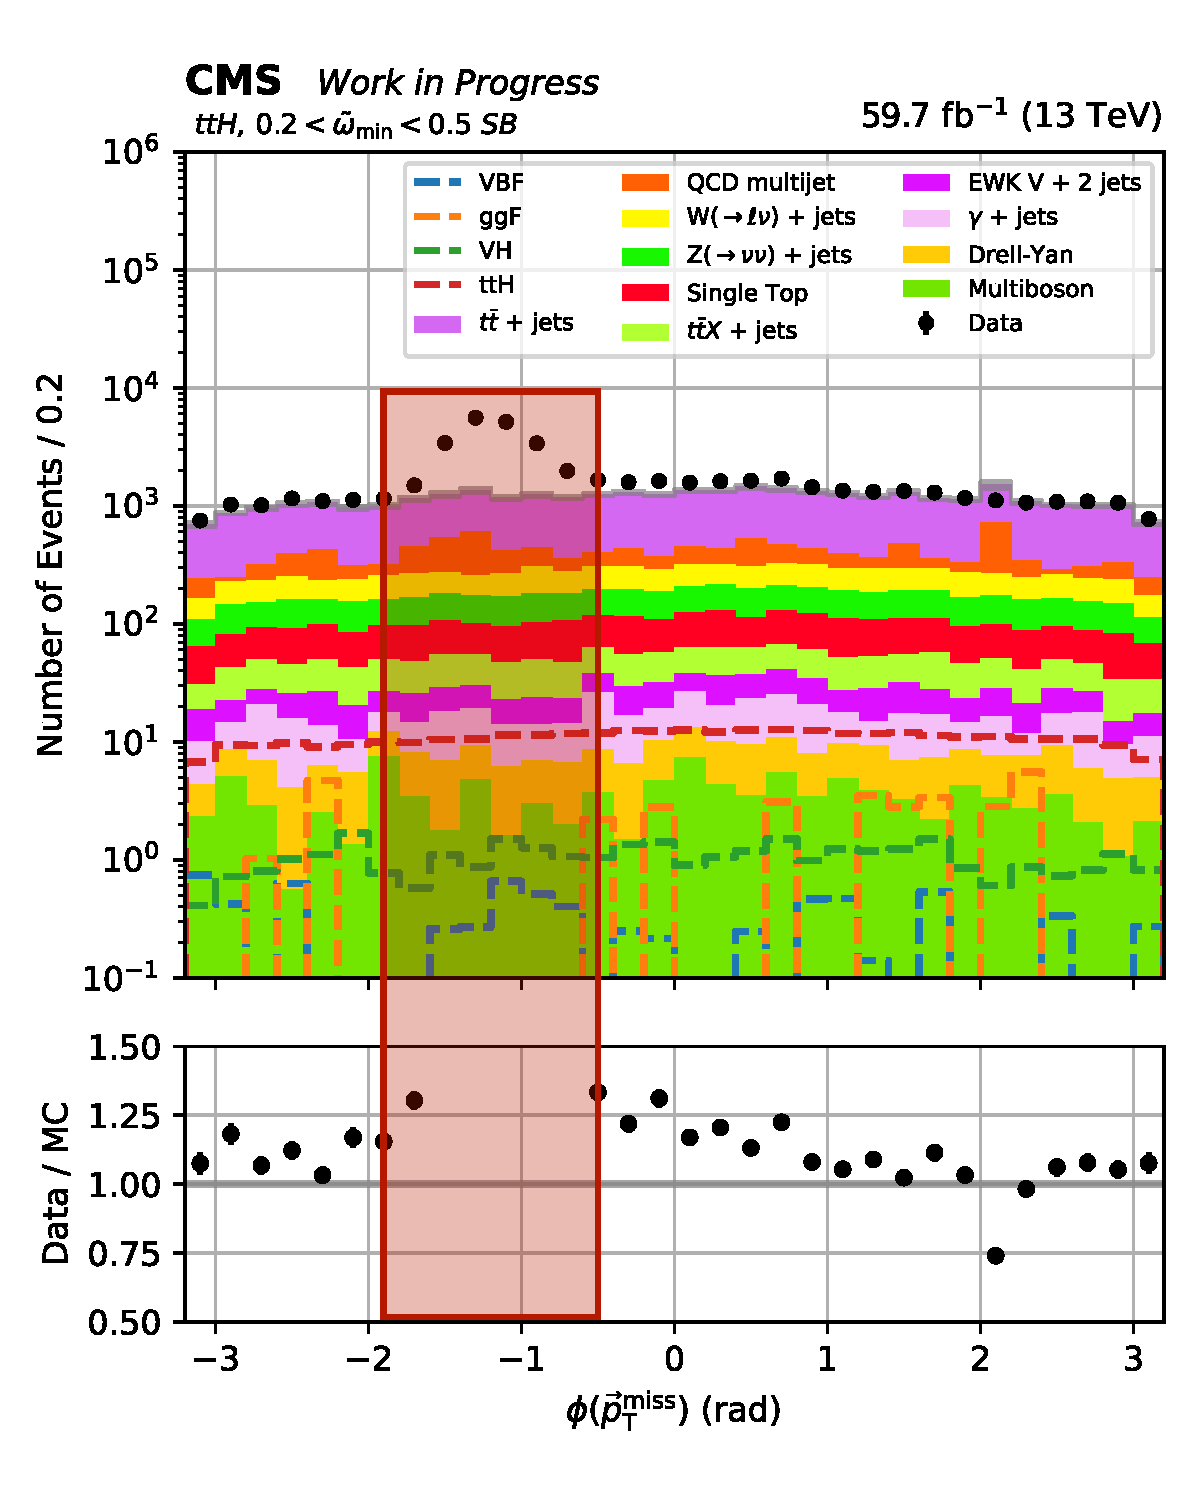
\includegraphics[width=\textwidth]{figures/hem_issue/sideband_4/met_phi_ttH_before_annotated.pdf}
        \caption{\ttH category}
    \end{subfigure}
    \hspace{0.05\textwidth}
    \begin{subfigure}[b]{0.34\textwidth}
        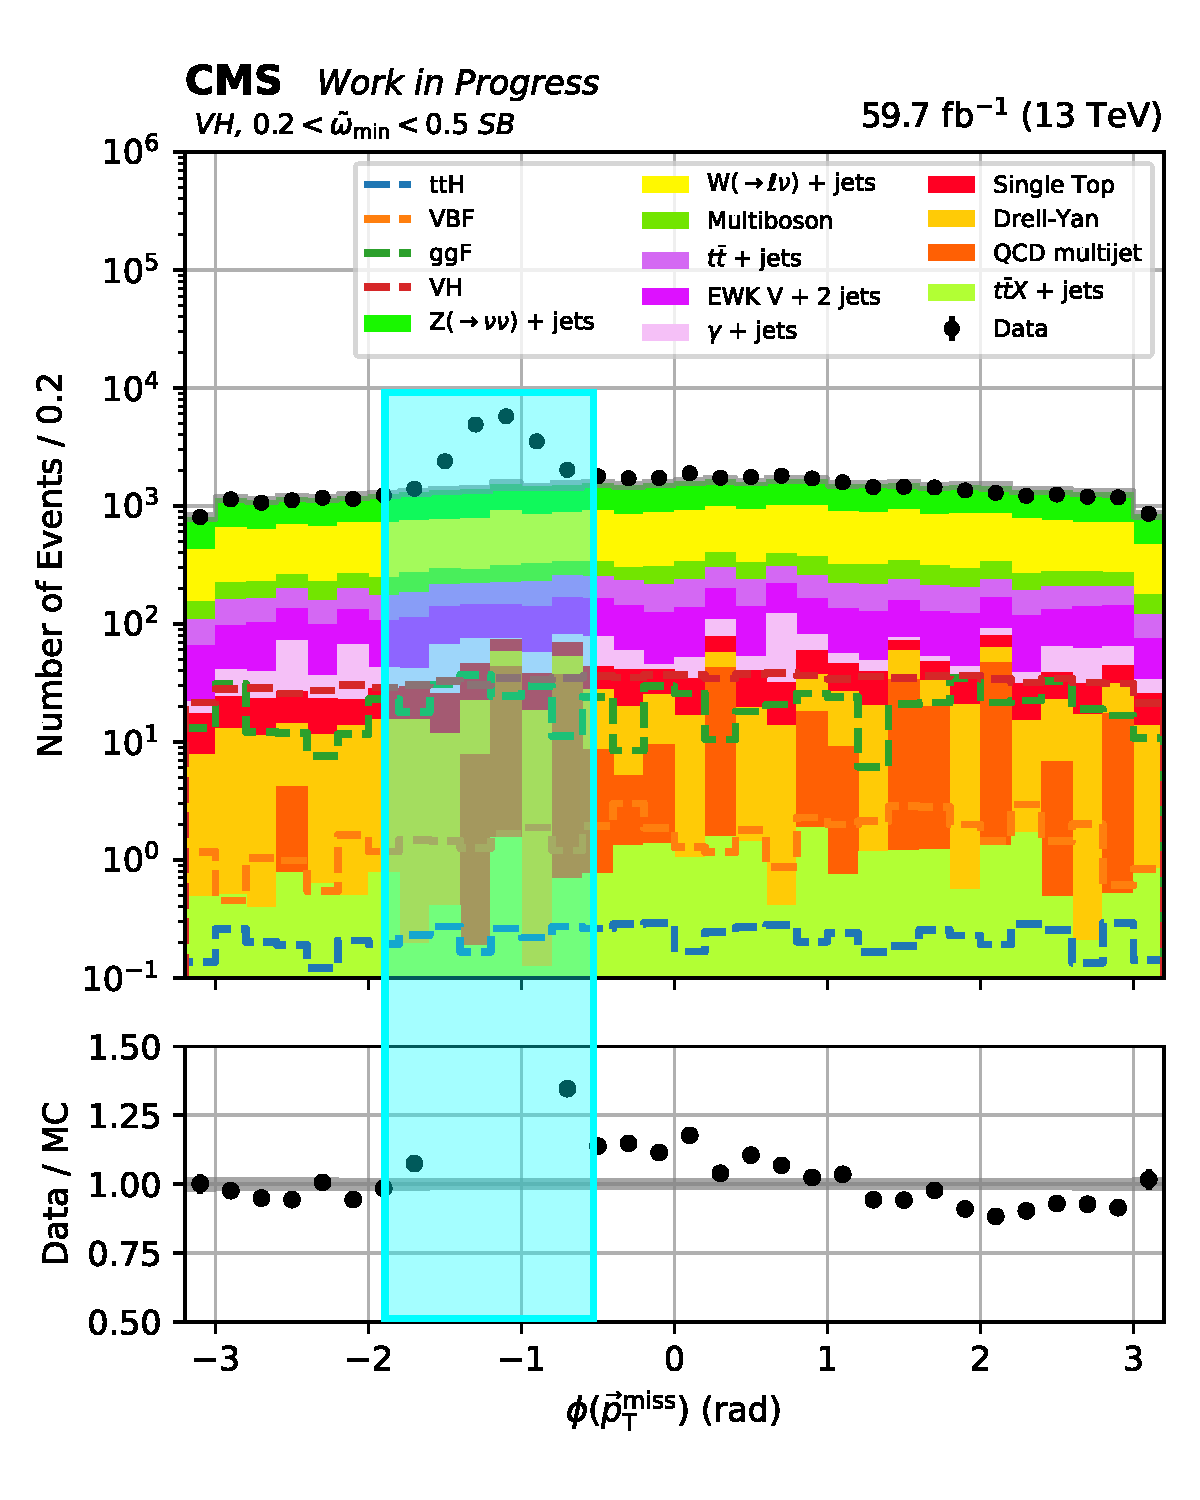
\includegraphics[width=\textwidth]{figures/hem_issue/sideband_4/met_phi_VH_before_annotated.pdf}
        \caption{\VH category}
    \end{subfigure}
    \caption[The azimuthal angle of the \ptvecmiss in the \ttH and \VH categories before applying the selections designed to mitigate the HEM issue in 2018]{The azimuthal angle of the \ptvecmiss in the \ttH and \VH categories before applying the selections designed to mitigate the HEM issue in 2018. The loose \omegaTilde \gls{SB} is used to demonstrate the effect since it kinematically resembles the signal region, and the data--simulation discrepancy can be removed while still blind in said region. A red box encloses the sector that is removed by the selection applied in the signal region and \glspl{SB}.}
    \label{fig:htoinv_hem_issue_met_phi}
\end{figure}

\begin{figure}[htbp]
    \centering
    \begin{subfigure}[b]{0.34\textwidth}
        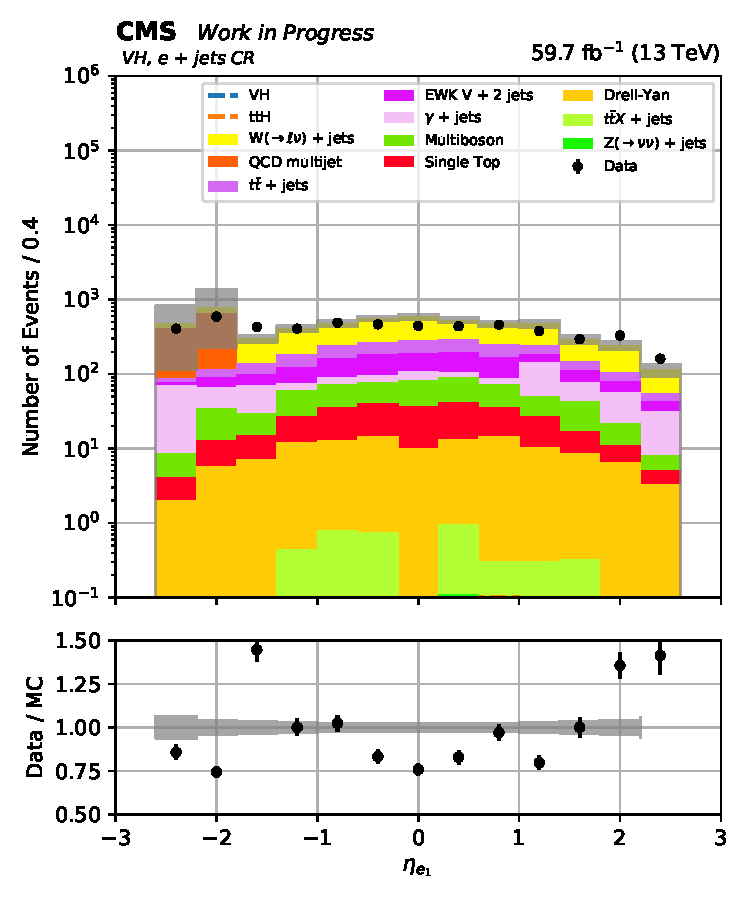
\includegraphics[width=\textwidth]{figures/hem_issue/region_3/leadLepton_eta_VH_before.pdf}
        \caption{$\eta_{\Pe}$ before cut}
    \end{subfigure}
    \hspace{0.05\textwidth}
    \begin{subfigure}[b]{0.34\textwidth}
        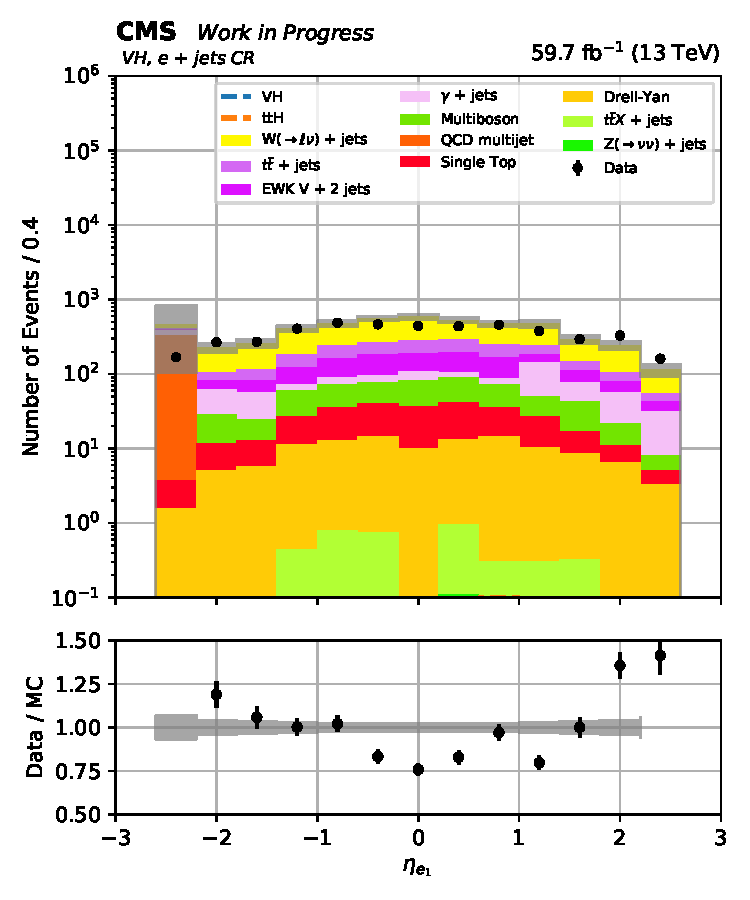
\includegraphics[width=\textwidth]{figures/hem_issue/region_3/leadLepton_eta_VH_after.pdf}
        \caption{$\eta_{\Pe}$ after cut}
    \end{subfigure}
    \caption[The psuedorapidity of the electron in the \VH category of the \singleEleCr \gls{CR} before applying the selection designed to mitigate the HEM issue in 2018]{The psuedorapidity of the electron in the \VH category of the \singleEleCr \gls{CR} before applying the selection designed to mitigate the HEM issue in 2018.}
    \label{fig:htoinv_hem_issue_lepton_eta}
\end{figure}

% Figures from 29th May, 2020


%=========================================================


\section{Categorisation of the non-VBF production modes}
\label{sec:htoinv_categorisation}

% This section is up-to-date as of 15th May.

To extract maximum sensitivity to the \higgstoinv decay from the analysis, categories are established to target each of the production modes. From first principles, the topologies outlined in Chpt.~\ref{subsec:theory_higgs_production_modes} provide an initial direction of the expected structure. Steps are taken to ensure the categories that target the production mechanism---and the subcategories that capitalise on specific topologies within the mechanism---are orthogonal. An additional angular variable cut based on optimisation studies in Chpt.~\ref{subsec:htoinv_cat_optimisation} is also implemented, devising the categories in Tab.~\ref{tab:htoinv_categories}.

\begin{table}[htbp]
    \centering
    \begin{tabular}{cccccccc}
        \hline\hline
        Category & Subcategory & \njet & \nbjet & \nBoostedTop & \nBoostedV & \mjj & Angular variable \\
        \hline
        \multirow{9}{*}{\ttH} & 2Boosted & $\geq \text{0}$ & $\geq \text{0}$ & \multicolumn{2}{c}{2} & \multirow{9}{*}{---} & \multirow{9}{*}{$\omegaTilde > \text{0.5}$} \\
        & 1t0b & $\geq \text{3}$ & 0 & 1 & 0 \\
        & 1t1b & $\geq \text{3}$ & 1 & 1 & 0 \\
        & 1W1b & $\geq \text{3}$ & 1 & 0 & 1 \\
        & 1W2b & $\geq \text{3}$ & 2 & 0 & 1 \\
        & 5j1b & 5 & 1 & 0 & 0 \\
        & 6j1b & $\geq \text{6}$ & 1 & 0 & 0 \\
        & 5j2b & 5 & $\geq \text{2}$ & 0 & 0 \\
        & 6j2b & $\geq \text{6}$ & $\geq \text{2}$ & 0 & 0 \\\hline
        \multirow{4}{*}{\VH} & 2j0b & 2 & 0 & 0 & 0 & $\in [\text{65}, \text{105})$ & \multirow{4}{*}{$\omegaTilde > \text{0.5}$} \\
        & 2j1b & 2 & 1 & 0 & 0 & $\in [\text{65}, \text{105})$ \\
        & 2j2b & 2 & 2 & 0 & 0 & $\in [\text{65}, \text{105})$ \\
        & 1V & 0 & 0 & 0 & 1 & ---\\\hline
        \multirow{4}{*}{\ggH}& 2jM & 2 & 0 & 0 & 0 & $\notin [\text{65}, \text{105})$ & \multirow{4}{*}{$\omegaTilde > \text{0.7}$} \\
        & 3j & 3 & 0 & 0 & 0 & ---\\
        & 4j & 4 & 0 & 0 & 0 & ---\\
        & 5j & $\geq \text{5}$ & 0 & 0 & 0 & ---\\\hline
        \multirow{2}{*}{Monojet}& 0b & 1 & 0 & 0 & 0 & \multirow{2}{*}{---} & \multirow{2}{*}{$\mindphiJetMet > \text{2.5}$}\\ % Replaced \dphiFj with this to prevent overfull hbox
        & 1b & 1 & 1 & 0 & 0 &  \\\hline\hline
    \end{tabular}
    \caption[Categorisation of the \ttH, \VH and \ggH production modes in the analysis]{Categorisation of the \ttH, \VH and \ggH production modes in the analysis. Each subcategory highlights one of the possible final states of the mechanism, accounting for inefficiencies in object tagging or reconstruction. In the \ggH 2jM subcategory, the dijet mass requirement ensures orthogonality with \VH 2j0b.}
    \label{tab:htoinv_categories}
\end{table}

The monojet category resembles the search in Ref.~\citenum{Sirunyan:2017jix}and primarily targets the \ggH mode, but is separated to distinguish it from the categories we have developed specifically for the analysis.

The number of boosted top quark- and vector boson-tagged \glspl{jet} (\nBoostedTop and \nBoostedV, respectively) are defined in Chpt.~\ref{subsec:htoinv_deepak8}. In the \ttH 2Boosted category, if $\nBoostedV = \text{2}$ we also require $\nbjet \geq \text{1}$ for confidence that the \PVec boson originates from a decaying \Ptop quark.

In the table, the number of \glspl{jet} \njet refers specifically to the number of AK4-clustered \glspl{jet} that do not overlap with a boosted \Ptop or \PVec \gls{jet} to avoid double counting objects, i.e., an AK4 \gls{jet} within $\Delta R < \text{0.8}$ of a boosted object does not count toward the \njet requirement in the subcategory definition. The same treatment is applied to \glspl{bjet} as well. This only applies to the categorisation and does not affect selections made on \glspl{jet} or \glspl{bjet} in Chpt.~\ref{sec:htoinv_event_selection}.

For categorisation and the analysis altogether, \njet and \nbjet are counted independently, so no overlap removal is performed. For example, the \VH 2j2b requires two \glspl{jet}, both of which are \Pbottom-tagged.

In the \ttH and \VH categories, ancillary groupings of subcategories may be of interest: 2Boosted, 1t0b, 1t1b, 1W1b, and 1W2b target boosted decays of the top quark and may be collectively designated the ``\ttH boosted'' category; resolved decays are the focus of the remaining subcategories, appropriately named the ``\ttH resolved'' category; then, assembling the 2j0b, 2j1b, and 2j2b \VH subcategories elicits the ``\VH resolved'' moniker. Low yields may be observed in individual subcategories, so using these grouped alternatives is useful to quickly inspect the wider effect of changes to the analysis.


%=========================================================


\subsection{Classifying boosted topologies from top quarks, and \texorpdfstring{\PW}{W} and \texorpdfstring{\PZ}{Z} bosons}
\label{subsec:htoinv_deepak8}

Many traditional methods have been developed to tag \glspl{jet} originating from heavy particles, such as top quarks, vector bosons and Higgs bosons. Though, there are limitations with all of these, and in the era of machine learning a plethora of new tools have arisen. One such algorithm---\deepakeight---has been developed by physicists in \acrshort{cms} to classify \glspl{jet} that originate from numerous heavy particles. In this analysis, we pay specific interest to those coming from top quarks and vector bosons in order to assist the categorisation of the \ttH and \VH signals. The number of tagged \glspl{jet} in an event inform the boosted subcategories, as seen in Tab.~\ref{tab:htoinv_categories}. The design and optimisation of the algorithm is described in Ref.~\citenum{CMS-PAS-JME-18-002}.\footnote{Not sure if I should give a summary of the development and features of the algorithm here.}

We employ the ensuing selections to AK8 \glspl{jet} to classify them, as recommended by the DeepAK8 developers:
\medskip
\begin{easylist}[itemize]
    \ListProperties(Style*=-- , Style2*=$\circ$ , Hang=true, FinalMark={)})
    & Boosted top:
    && $\pt > \text{400}\GeV$
    && $\text{105} < m_{\mathrm{SD}} < \text{210} \GeV$
    && \Ptop vs. \acrshort{qcd} discriminator score with the ``loose'' working point (2.5\,\% mis-tag rate)
    && Tight ID requirement for AK8 \glspl{jet}

    & Boosted \PVec:
    && $\pt > \text{200}\GeV$
    && $\text{65} < m_{\mathrm{SD}} < \text{105} \GeV$
    && \PW vs. \acrshort{qcd} discriminator score with the ``loose'' working point (5\,\% mis-tag rate)
    && Tight ID requirement for AK8 \glspl{jet}
\end{easylist}

\medskip

\noindent{}Orthogonality is ensured between the two classifications through the softdrop mass $m_{\mathrm{SD}}$~\cite{Larkoski:2014wba} window. We also use the loose working points to maximise the number of events that remain in the relevant categories. Otherwise, we suffer from very poor statistics in some of the \glspl{CR}. The boosted \PVec \glspl{jet} are not further separated into \PW- and \PZ-tagged since the mass degeneracy makes this inherently difficult. After correspondence with the \deepakeight developers, we were reassured that we could use the \PW vs. \acrshort{qcd} discriminator to tag both \PW and \PZ \glspl{jet}. An additional recommendation was to use the nominal version of the tagger as opposed to the mass-decorrelated version. The performance improvements are noticeable, as shown in Ref.~\citenum{CMS-PAS-JME-18-002}, and we do not use a mass dimension for our fitting variable which would otherwise preclude the use of the latter version. Data-\acrshort{mc} scale factors to weight events containing these objects are described in Chpt.~[REF].


%=========================================================


\subsection{Optimisation of the categories}
\label{subsec:htoinv_cat_optimisation}

% This subsection, more than most, may be subject to change

While first principles are a good starting point to categorise events and accentuate the Higgs production modes, they allow much room for improvement. \acrshort{qcd} multijet is still a prominent background, especially in the \ttH and \ggH categories. Historically, variables such as \biasedDPhi and \alphat have been used to suppress it, as in the previous \acrlong{susy} analysis I was a part of.

Recently, more elaborate variables have been developed to better remove multijet background events in analyses with hadronic final states. Colleagues at the University of Bristol have designed a family of them: \minChi, \omegaHat, and \omegaTilde~\cite{Sakuma:2018xrq}. These show noticeable improvement over previous variables (particularly \biasedDPhi, which is used as a benchmark for comparisons). Optimisation was performed for these variables on a per-category, over a per-subcategory, basis to avoid excessive fine tuning for the many subcategories in the analysis. After investigating each variable, \omegaTilde was chosen for the \ttH, \VH, and \ggH categories. A more traditional \mindphiJetMet was selected for the monojet category, as the aforementioned ones typically perform better at higher \gls{jet} multiplicity.

Various metrics (or figures of merit) were considered for the threshold to cut on the given angular variable. In a counting experiment, a known Possion-distributed background $B$ yields a statistical uncertainty---assuming one standard deviation---of $\sqrt{B}$. A signal count $S$ can then be statistically significant (i.e., unlikely to be a statistical fluctuation of the background) if it is greater than the uncertainty on the background. This, somewhat simplistic, method gives the standard deviation for the expected signal with respect to background---often just referred to as the \emph{expected significance} $Z$---as
\begin{equation}
Z_{\mathrm{Poisson}} = \frac{S}{\sqrt{B}}
\label{eq:s_over_root_b}
\end{equation}

An estimate of the overall effect of systematic uncertainties on the background $\bkgsystuncert$ can also be incorporated, leading to
\begin{equation}
Z_{\mathrm{Poisson}} = \frac{S}{\sqrt{B + (\bkgsystuncert B)^2}}
\label{eq:s_over_root_b_systs}
\end{equation}

Another figure of merit is to use the significance from an ``Asimov dataset''---which replaces the [ensemble] of different datasets by a single representative one~\cite{Cowan:2010js}. The median significance can then be extracted. Colloquially ascribed the \emph{Asimov significance}. In many fields, including particle physics, a likelihood ratio is used for hypothesis testing. This is described in the context of the analysis in Chpt.~\ref{sec:htoinv_satistical_treatment}. The asymptotic limit, where the sample size is large (as in the case for \acrshort{lhc} data and simulation), can also be exploited as a property within the likelihood model. In this regime, the Asimov significance $Z_{\mathrm{Asimov}}$ can be expressed as  % EXPLAIN. LOOK IN statistical_significance/ folder in Downloads/
\begin{equation}
Z_{\mathrm{Asimov}} = \sqrt{2 \left( (S + B) \cdot \ln\left(1 + \frac{S}{B} \right) - S \right)}
\label{eq:asimov_significance}
\end{equation}

reducing to Eq.~\ref{eq:s_over_root_b} for $S \ll B$. Including a systematic uncertainty expands Eq.~\ref{eq:asimov_significance} to
\begin{equation}
    \begin{gathered}  % use gathered environment to centre each row in the equation, while avoiding each row having its own equation number
Z_{\mathrm{Asimov}} = \sqrt{2 \left( (S + B) c_1 - \frac{B^2}{\bkgsystuncert^2}c_2 \right)}, \ \text{where} \\[1em]
c_1 = \ln\left( \frac{(S + B) \cdot (B + \bkgsystuncert^2)}{B^2 + (S + B)\bkgsystuncert^2} \right), \ c_2 = \ln\left( 1 + \frac{\bkgsystuncert^2 S}{B(B + \bkgsystuncert^2)} \right)
    \end{gathered}
\label{eq:asimov_significance_systs}
\end{equation}

While these are quantitative measures of the sensitivity with an given analysis configuration, they are only a guide to inform an analyst of a more specific area of phase space to consider, rather than providing a precise cut for the given variable. To derive the appropriate cut for each category in the final column of Tab.~\ref{tab:htoinv_categories}, we first processed all simulated signal and background events through the analysis. They were categorised according to the aforementioned table (of course, excluding the angular variable cut). For each subcategory, the significances for both methods were calculated, with and without an estimated 5\,\% systematic uncertainty on the background distribution. To estimate the significance for a category, the significances for each subcategory were summed in quadrature. Fig.~\ref{fig:htoinv_category_optimisations_significances} demonstrates the results as a function of \omegaTilde for the \ttH, \VH, and \ggH categories with the 2017 datasets.

\begin{figure}[htbp]
    \centering
    \begin{subfigure}[b]{0.27\textwidth}
        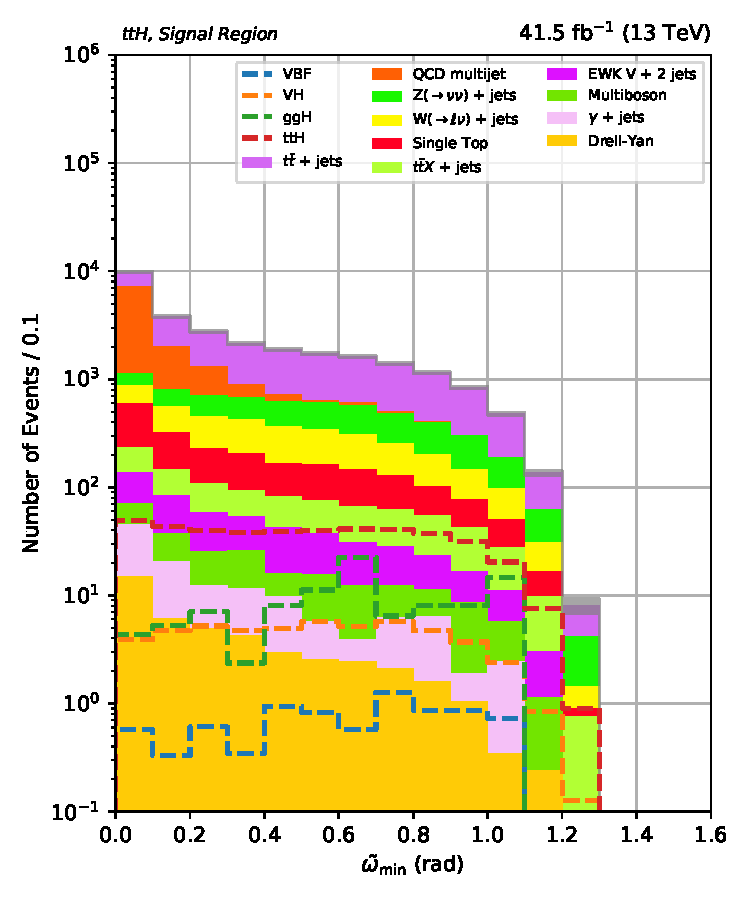
\includegraphics[width=\textwidth]{figures/category_optimisations/min_omega_tilde_ttH.pdf}
        \caption{\ttH category}
    \end{subfigure}
    \hfill
    \begin{subfigure}[b]{0.27\textwidth}
        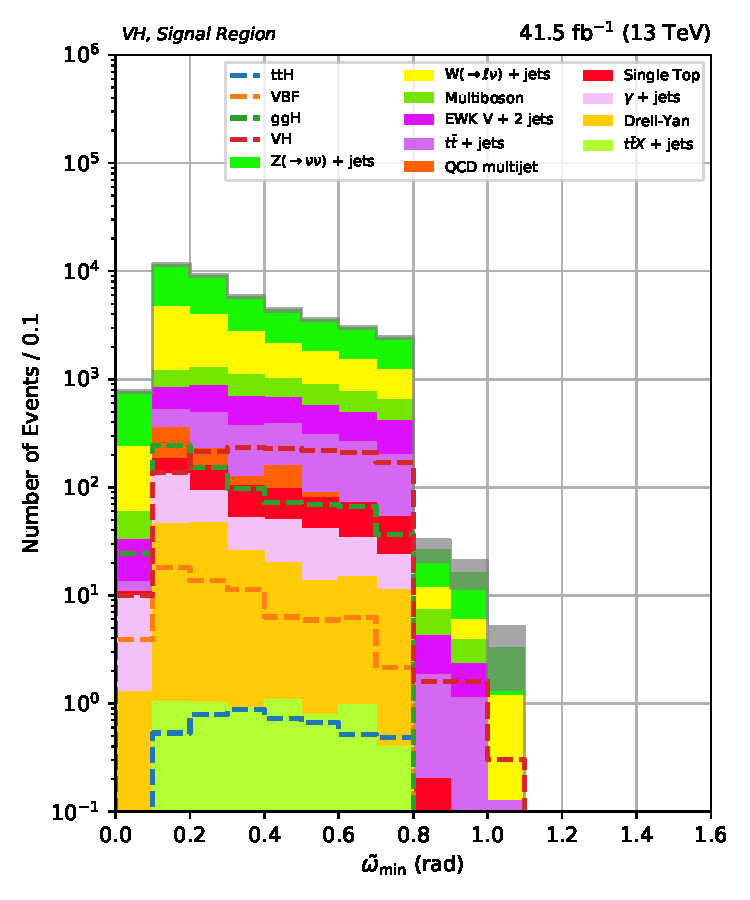
\includegraphics[width=\textwidth]{figures/category_optimisations/min_omega_tilde_VH.pdf}
        \caption{\VH category}
    \end{subfigure}
    \hfill
    \begin{subfigure}[b]{0.27\textwidth}
        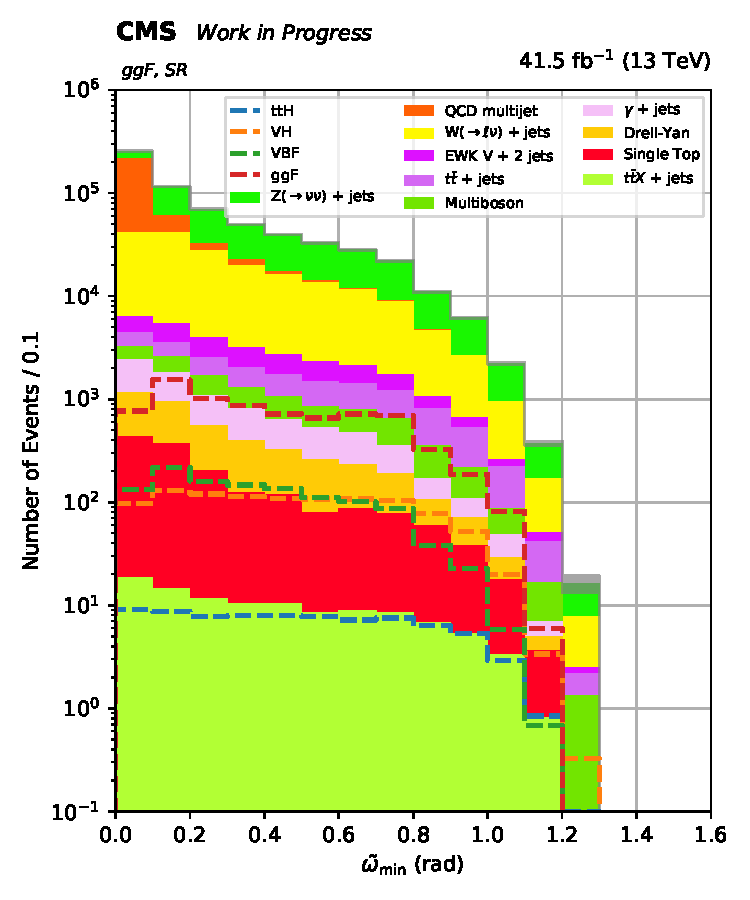
\includegraphics[width=\textwidth]{figures/category_optimisations/min_omega_tilde_ggF.pdf}
        \caption{\ggH category}
    \end{subfigure}

    \begin{subfigure}[b]{0.27\textwidth}
        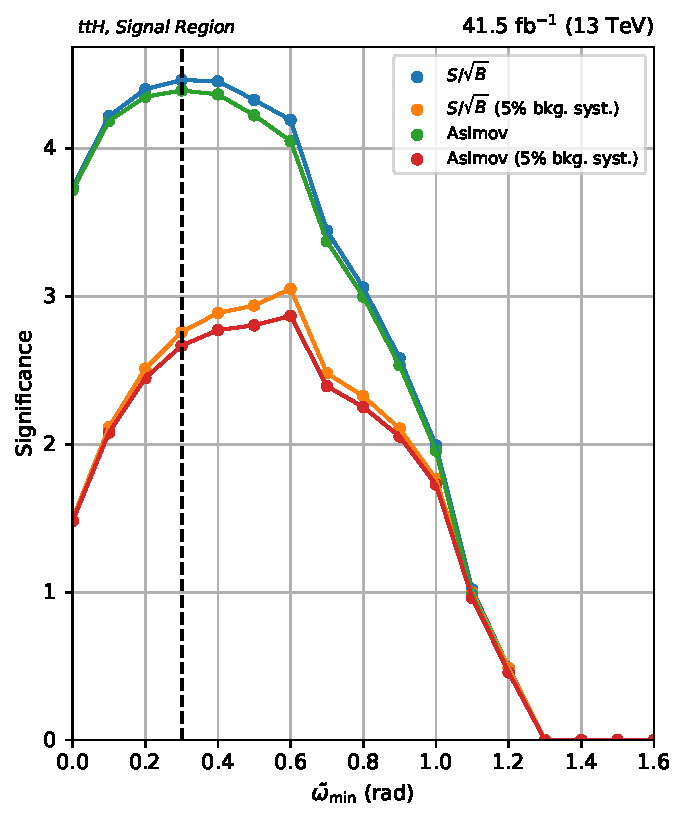
\includegraphics[width=\textwidth]{figures/category_optimisations/significance_ttH_min_omega_tilde_all.pdf}
        \caption{Significance of cut in \ttH category}
    \end{subfigure}
    \hfill
    \begin{subfigure}[b]{0.27\textwidth}
        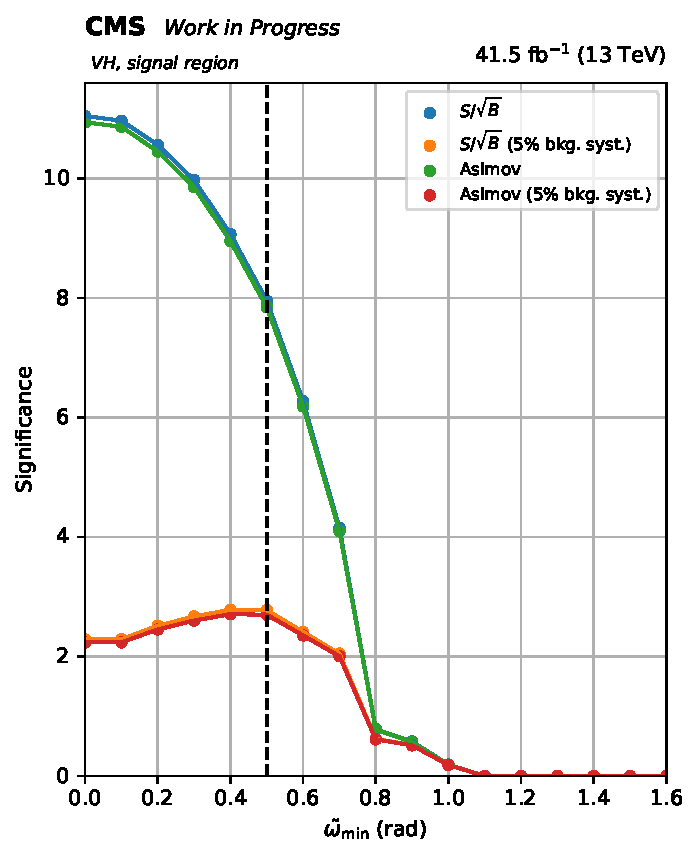
\includegraphics[width=\textwidth]{figures/category_optimisations/significance_VH_min_omega_tilde_all.pdf}
        \caption{Significance of cut in \VH category}
    \end{subfigure}
    \hfill
    \begin{subfigure}[b]{0.27\textwidth}
        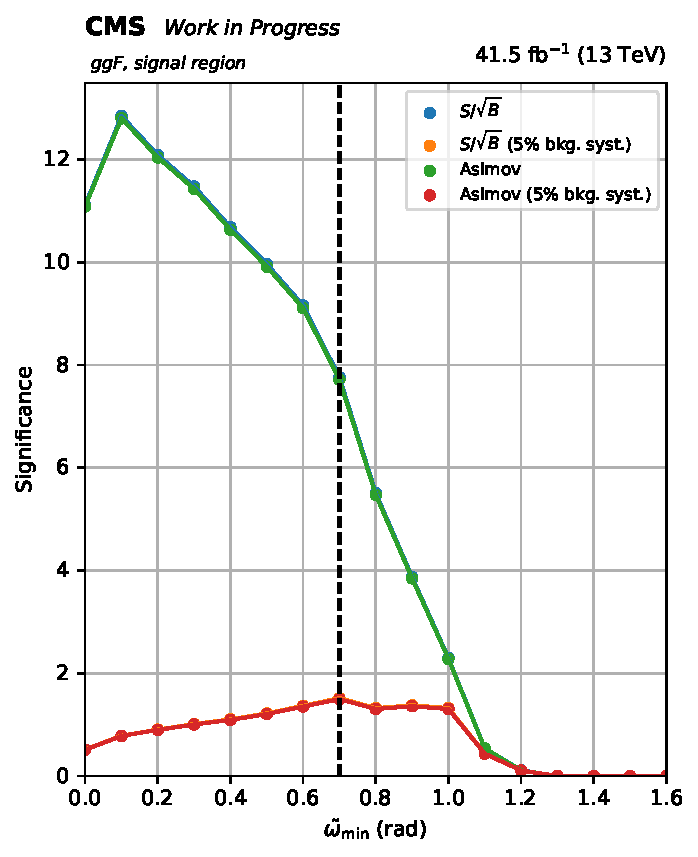
\includegraphics[width=\textwidth]{figures/category_optimisations/significance_ggF_min_omega_tilde_all.pdf}
        \caption{Significance of cut in \ggH category}
    \end{subfigure}
    \caption[Distributions of \omegaTilde in the signal region in the \ttH, \VH, and \ggH categories, along with the significance---using several figures of merit---if a cut is placed to the right of a given value]{Top row: distributions of \omegaTilde in the signal region in the \ttH, \VH, and \ggH categories. Bottom row: the significance---using several figures of merit---if a cut is placed to the right of a given value of \omegaTilde in each category. The black dotted line indicates the threshold used in the analysis. These are showcased after the analysis-level selection on signal and background simulation for the 2017 data-taking era.}
    \label{fig:htoinv_category_optimisations_significances}
\end{figure}

% Figures from 1st June 2020. When remaking, ensure the colours of the signal lines are consistent, and the legend doesn't overlap with the distribution

It is obvious that the shapes and magnitudes of the significance distributions are sensitive to the inclusion of an estimated systematic uncertainty. Increasing its size affects the shape little, though impacts the magnitude more significantly. In bins with high background occupancy, even a small systematic uncertainty can wash out traces of signal. The thresholds chosen for \omegaTilde do not necessarily maximise the significance---where the Asimov method with $\bkgsystuncert = \text{5\,\%}$ was the leading choice---but to sufficiently separate signal and background, while not removing too many events. The \glspl{CR} in the analysis perform better estimations of their responsible backgrounds when adequately populated. Reducing the background too greatly with the \omegaTilde cut can therefore cause problems in multiple aspects of the analysis.


%=========================================================


\subsection{Binning}
\label{subsec:htoinv_binning}

In addition to the categories above, events are placed in bins of \ptmiss as that distribution is expected to maximally differentiate signal and background in the final fit (see Chpt.~\ref{sec:htoinv_satistical_treatment}). Since the number of events can significantly differ between categories in the different regions of the analysis, a global binning configuration is inadequate. For each category, the number and widths of the bins are tuned to ensure sufficient statistical precision. These schemes are tied to the category, so are reflected in all regions such that transfer factors from the background estimation methods are calculated on a bin-by-bin basis.\footnote{Not sure if this subsection should instead go in the fit discussion. But as I haven't written any of that, I'll leave it here for now.}


%=========================================================


\section{Signal region, control region, and sideband definitions}
\label{sec:region_definitions}

Several regions of phase space are explored in the analysis. The signal region is accompanied by \glspl{CR} and \glspl{SB} to aid in the prediction of certain backgrounds, as explained below. The preselection is applied to every region, so they are separated by the \acrshort{cms} datasets used, the \acrlong{hlt} requirements, and object and/or kinematic selections.

% This section is up-to-date as of 14th May


%=========================================================


\subsection{The signal region}
\label{subsec:htoinv_signal_region}

The signal region is the area of parameter space where we expect the signal to manifest, and the background to be reduced sufficiently that the potential presence of signal in data can be statistically verified. In this analysis, only hadronic final states are permitted. Events with leptons, photons and taus meeting the ``loose'' or ``veto'' criteria in Chpt.~\ref{sec:analysis_objects} are not explicitly vetoed, however, but are given a weight as described in Chpt.~\ref{subsubsec:veto_sel_weights}.

Events must satisfy a logical \texttt{OR} of \acrshort{hlt} cross-triggers for \acrlong{pf} \ptmiss and \mht calculated without muons, and at least one \gls{jet} fulfilling the tight ID criteria (see Chpt.~\ref{sec:analysis_objects}). The triggers are illustrated in Tab.~\ref{tab:htoinv_SR_triggers}.

\begin{table}[htbp]
    \centering
    \begin{tabular}{ccccc}
        \hline\hline
        Year & $p_{\mathrm{T}}^{\mathrm{miss,\, \not\Pmu}}$ (\GeVns) & $H_{\mathrm{T}}^{\mathrm{miss,\, \not\Pmu}}$ (\GeVns) & $\HT$ (\GeVns) & $\njet$ with tight ID \\ \hline
        \multirow{4}{*}{2016} & 90 & 90 & --- & $\geq \text{1}$ \\
        & 100 & 100 & --- & $\geq \text{1}$ \\
        & 110 & 110 & --- & $\geq \text{1}$ \\
        & 120 & 120 & --- & $\geq \text{1}$ \\
        \hline
        \multirow{2}{*}{2017} & 120 & 120 & --- & $\geq \text{1}$ \\
        & 120 & 120 & 60 & $\geq \text{1}$ \\
        \hline
        2018 & 120 & 120 & --- & $\geq \text{1}$ \\
        \hline\hline
    \end{tabular}
    \caption[The trigger thresholds required for events to enter the signal region in each data taking year]{The trigger thresholds required for events to enter the signal region in each data taking year. Each quantity is computed with the \gls{particleflow} at \acrshort{hlt} level. The variables \ptmiss and \mht do not include muons in the calculations.}
    \label{tab:htoinv_SR_triggers}
\end{table}

\begin{figure}[htbp]
    \centering
    \begin{subfigure}[b]{0.24\textwidth}
        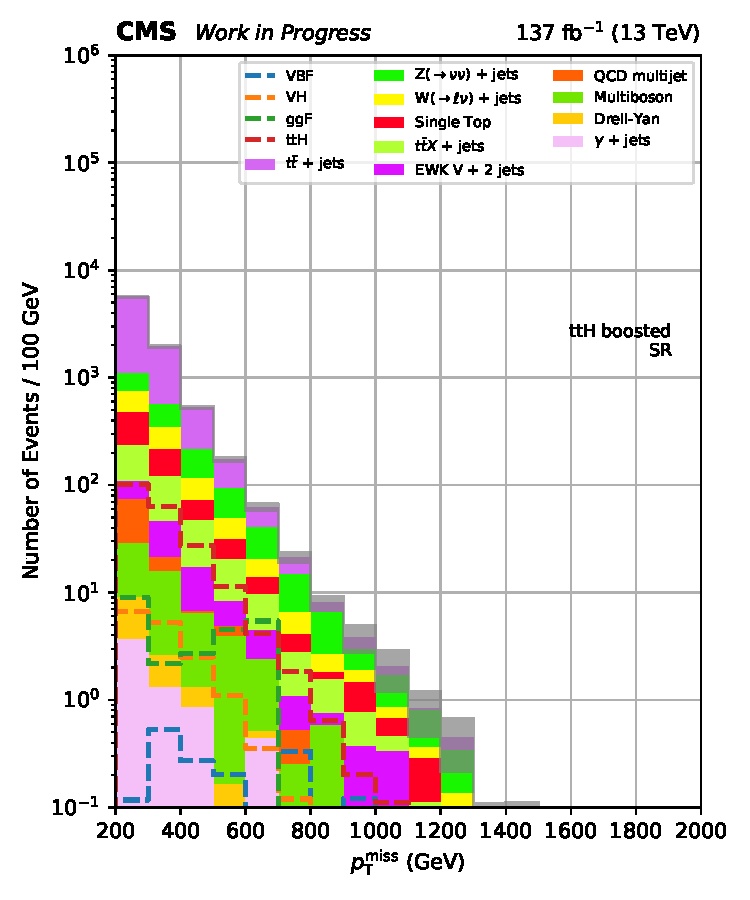
\includegraphics[width=\textwidth]{figures/region_plots/2016to18/region_0/ttH_boosted.pdf}
        \caption{\ttH boosted}
    \end{subfigure}
    \hfill
    \begin{subfigure}[b]{0.24\textwidth}
        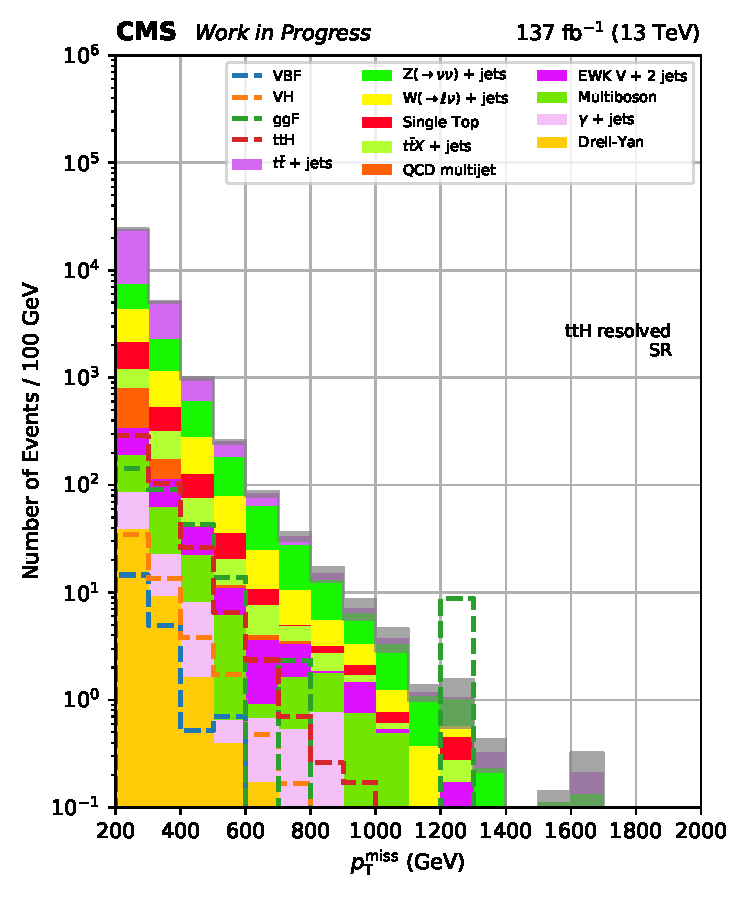
\includegraphics[width=\textwidth]{figures/region_plots/2016to18/region_0/ttH_resolved.pdf}
        \caption{\ttH resolved}
    \end{subfigure}
    \begin{subfigure}[b]{0.24\textwidth}
        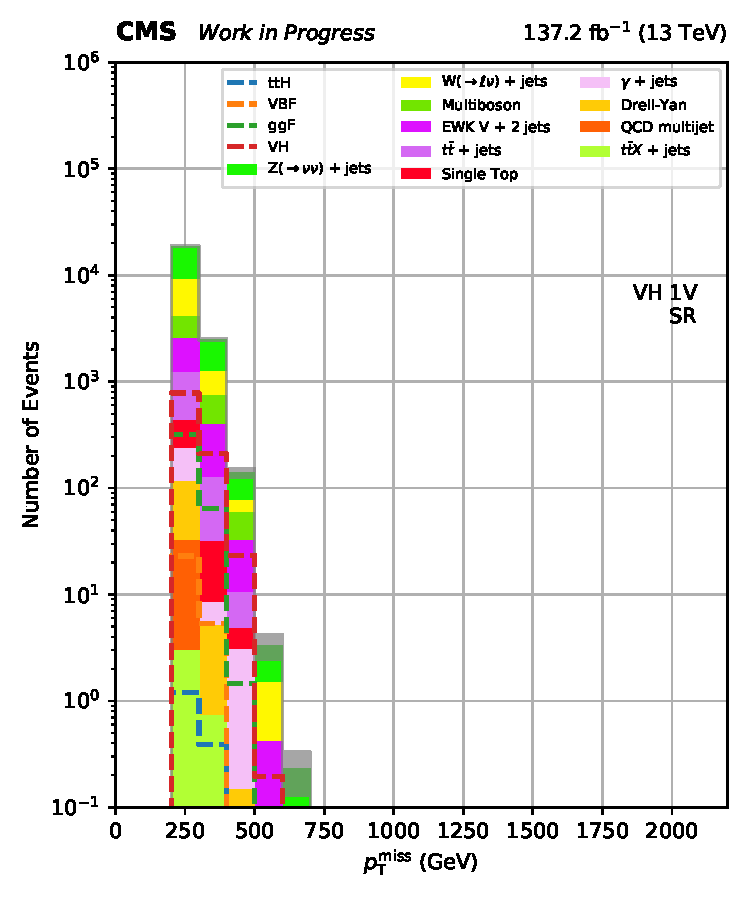
\includegraphics[width=\textwidth]{figures/region_plots/2016to18/region_0/VH_1V.pdf}
        \caption{\VH 1V}
    \end{subfigure}
    \hfill
    \begin{subfigure}[b]{0.24\textwidth}
        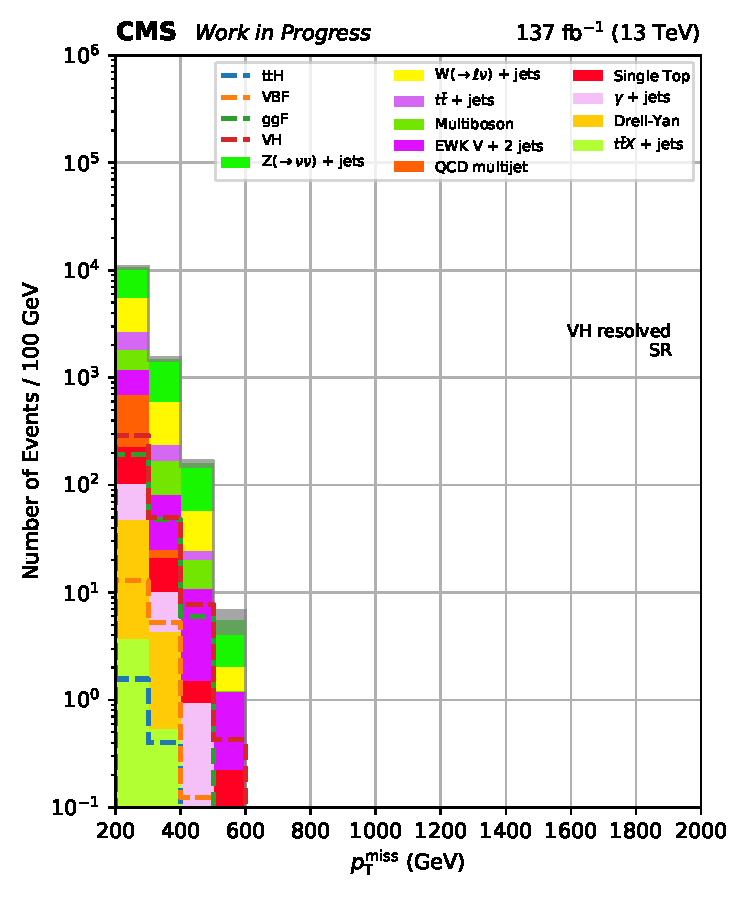
\includegraphics[width=\textwidth]{figures/region_plots/2016to18/region_0/VH_resolved.pdf}
        \caption{\VH resolved}
    \end{subfigure}
    \caption[Pre-fit yields of the \ptmiss distribution in the signal region for the combined boosted and resolved categories for the \ttH and \VH processes, using simulation derived for each year in Run-2 and scaled to the required luminosity]{Pre-fit yields of the \ptmiss distribution in the \singleMuCr \gls{CR} for the combined boosted and resolved categories for the \ttH and \VH processes, using simulation derived for each year in Run-2 and scaled to the required luminosity.}
    \label{fig:htoinv_sr_yields_comb2016to18}
\end{figure}

% Figures from 29th May, 2020


%=========================================================


\subsection{Control regions}
\label{subsec:htoinv_control_regions}

\Glspl{CR} serve two complementary purposes in many analyses: the prediction of certain backgrounds that dominate in the signal region, as a more accurate method than using the yields directly from \acrlong{mc}; and to validate the data, \acrshort{mc}, and corrections or weights applied. They are orthogonal to the signal region and to each other by way of lepton or photon requirements, and by triggers that may pertain to those objects. \Glspl{CR} are also designed to, ideally, be devoid of signal. Contamination is sometimes present, but at a very small level. Five \glspl{CR} are used in the analysis: \singleMuCr, \doubleMuCr, \singleEleCr, \doubleEleCr, and \singlePhotonCr. The criteria for the objects---which are defined explicitly in Chpt.~\ref{sec:analysis_objects}---are summarised in the list below.
\medskip
\begin{easylist}[itemize]
    \easylistprops
    & \singleMuCr: one tight muon \tightMuon with $\pt > \text{20}\GeV$ and a transverse mass (as calculated in Eq.~\ref{eq:transverse_mass_massless}) in the range $\text{50} < \mtMuon < \text{110}\GeV$
    & \doubleMuCr: one tight muon \tightMuon with $\pt > \text{20}\GeV$, and one loose muon \looseMuon with $\pt > \text{10}\GeV$ that has opposite charge, with a combined invariant mass of $\text{60} < \doubleMuMass < \text{120}\GeV$
    & \singleEleCr: one tight electron \tightEle with $\pt > \text{40}\GeV$ and $\text{50} < \mtElectron < \text{110}\GeV$
    & \doubleEleCr: one tight electron \tightEle with $\pt > \text{40}\GeV$, and one veto electron \vetoEle with $\pt > \text{10}\GeV$ that has opposite charge, with a combined invariant mass of $\text{60} < \doubleEleMass < \text{120}\GeV$
    & \singlePhotonCr: one medium photon \mediumPhoton with $\pt > \text{230}\GeV$
\end{easylist}

\medskip

\noindent{}The transverse mass cuts in the single lepton \glspl{CR} reduce the effect of signal contamination, specifically from \ttH since its \mT generally eclipses that of \ttbar. The trigger requirements for the \singleMuCr and \doubleMuCr \glspl{CR} are the same as for the signal region (Tab.~\ref{tab:htoinv_SR_triggers}) since the same primary dataset is used.

The \singleEleCr and \doubleEleCr \glspl{CR} take advantage of the increased statistical power of two primary datasets in both 2016 and 2017, characterised by electron and photon triggers. In 2018, they were merged into a single $\Pe/\Pphoton$ primary dataset. Tabs.~\ref{tab:htoinv_ele_pd_triggers} and~\ref{tab:htoinv_photon_pd_triggers} elucidate how the trigger requirements are specified for each year. As before, each quantity and object is defined at \acrshort{hlt} level. If an event aims to enter the \singleEleCr or \doubleEleCr, and is from the dataset of \Pe-based triggers, the criteria for either of the two triggers for the given year in Tab.~\ref{tab:htoinv_ele_pd_triggers} must be satisfied. If an event aims to enter either \gls{CR} and is from the primary dataset of \Pphoton-based triggers, the failure of both of the electron triggers in Tab.~\ref{tab:htoinv_ele_pd_triggers} and the passing of any of the photon triggers in Tab.~\ref{tab:htoinv_photon_pd_triggers} are required. This condition avoids double counting events that also appear in the electron trigger-based dataset. In 2018, any of the year's triggers in Tabs.~\ref{tab:htoinv_ele_pd_triggers} and~\ref{tab:htoinv_photon_pd_triggers} may be satisfied. For \acrlong{mc} events, as they are not categorised by trigger, they may pass any of the triggers in either table for their respective year.\footnote{See if I can describe the trigger requirements in a more elegant way. Might be easier give the descriptions and actual HLT path names a bit earlier, then just reference the HLT path names in the list.}

\begin{table}[htbp]
    \centering
    \begin{tabular}{ccccc}
        \hline\hline
        Year & \Pe SC \ET threshold (\GeVns) & \Pe WP & Calorimeter ID & \acrshort{gsf} track-SC matching \\ \hline
        \multirow{2}{*}{2016} & 27 & Tight & --- & --- \\
        & 105 & --- & Very tight & Tight \\\hline
        \multirow{2}{*}{2017} & 35 & Tight & --- & --- \\
        & 115 & --- & Very tight & Tight \\\hline
        \multirow{2}{*}{2018} & 32 & Tight & --- & --- \\
        & 115 & --- & Very tight & Tight \\
        \hline\hline
    \end{tabular}
    \caption[The trigger requirements for events to enter the \singleEleCr or \doubleEleCr control regions, if they originate from the dataset of \Pe-based triggers]{The trigger requirements for events to enter the \singleEleCr or \doubleEleCr \glspl{CR}, if they originate from the dataset of \Pe-based triggers. Selections are on the transverse energy \ET of the supercluster (SC), the working point of the candidate electron, ID of the candidate in the calorimeters, and the matching between the \acrfull{gsf}-fitted track and supercluster, all at \acrshort{hlt} level.}
    \label{tab:htoinv_ele_pd_triggers}
\end{table}

For the \singlePhotonCr \gls{CR}, we take data from \acrshort{cms} originating only from the dataset of \Pphoton-based triggers. Data and \acrshort{mc} must satisfy any of the triggers from Tab.~\ref{tab:htoinv_photon_pd_triggers} for the respective year.

\begin{table}[htbp]
    \centering
    \begin{tabular}{ccc}
        \hline\hline
        Year & \Pphoton \ET threshold (\GeVns) & $H/E$ \\\hline
        \multirow{2}{*}{2016} & 165 & $< \text{0.1}$ \\
        & 175 & --- \\\hline
        2017 & 200 & --- \\\hline
        2018 & 200 & --- \\\hline\hline
    \end{tabular}
    \caption[The trigger requirements for events to enter the \singleEleCr, \doubleEleCr, or \singlePhotonCr control regions, if they originate from the dataset of \Pphoton-based triggers]{The trigger requirements for events to enter the \singleEleCr, \doubleEleCr, or \singlePhotonCr \gls{CR}, if they originate from the dataset of \Pphoton-based triggers. Selections are on the transverse energy \ET of the candidate, and the ratio of the candidate's central energy deposit in the \acrshort{hcal} to the \acrshort{ecal} ($H/E$), all computed at \acrshort{hlt} level.}
    \label{tab:htoinv_photon_pd_triggers}
\end{table}

As explained in Chpt.~\ref{subsec:objects_analysis_energy_sums}, the \ptvecmiss is recalculated for the \glspl{CR}. Using the \singleMuCr \gls{CR} as an example, the new \ptvecmiss is the vector sum of the old \ptvecmiss and the tight muon \ptvec. The single lepton \glspl{CR} estimate the semi-leptonic $\ttbarpjets$ and $\wtolnupjets$ backgrounds. In both cases, they may enter the signal region if the lepton is lost, becoming a source of \ptmiss. The dilepton and \singlePhotonCr regions consider \ztonunupjets. The former parallels the decay as it is enriched in \ztolplmpjets---possessing very similar kinematic properties while being much easier to detect, improving statistical accuracy. The latter region substitutes the \ztonunu decay with a photon.

The following figures reveal the pre-fit \ptmiss distributions in each \gls{CR} after the analysis-level selections with the full Run-2 dataset. The combined \ttH and \VH subcategories for boosted and resolved topologies are used to demonstrate the shapes and data--simulation agreement. Background estimation is performed separately for each year due to the differing running conditions, detector configuration, and the different effects or problems seen in the data.\footnote{Might not need to show all of these plots. They're just here for now, and can be tidied up later.}

\begin{figure}[htbp]
    \centering
    \begin{subfigure}[b]{0.24\textwidth}
        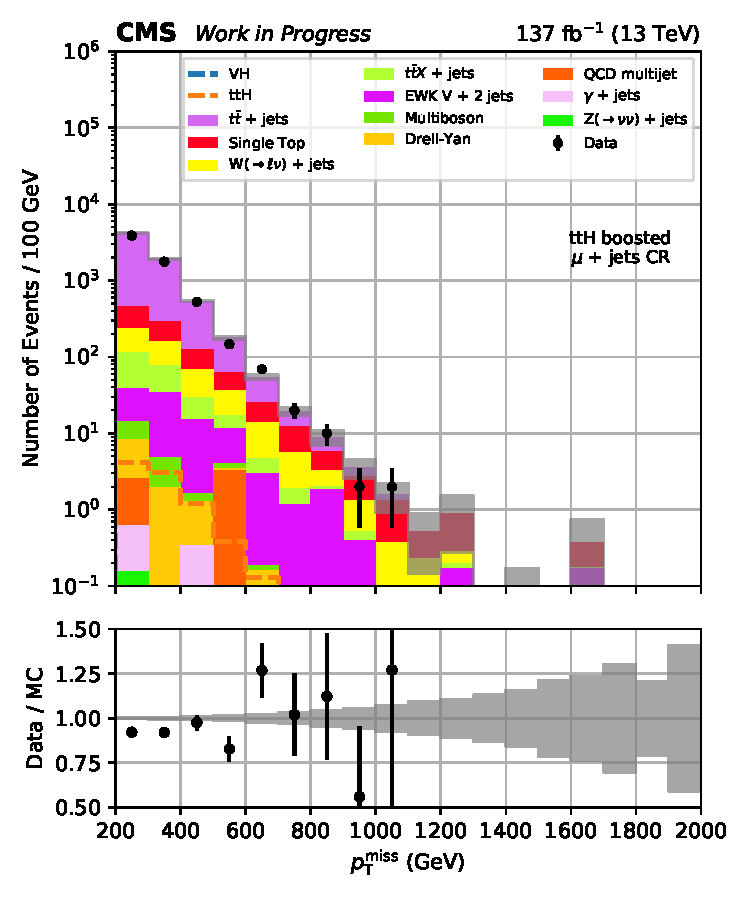
\includegraphics[width=\textwidth]{figures/region_plots/2016to18/region_1/ttH_boosted.pdf}
        \caption{\ttH boosted}
    \end{subfigure}
    \hfill
    \begin{subfigure}[b]{0.24\textwidth}
        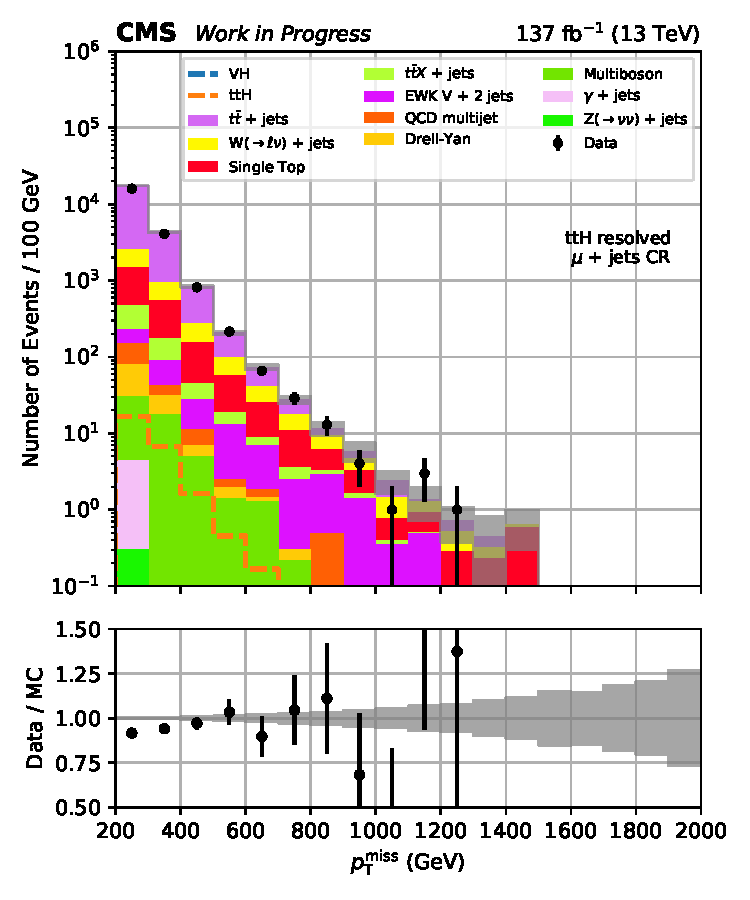
\includegraphics[width=\textwidth]{figures/region_plots/2016to18/region_1/ttH_resolved.pdf}
        \caption{\ttH resolved}
    \end{subfigure}
    \hfill
    \begin{subfigure}[b]{0.24\textwidth}
        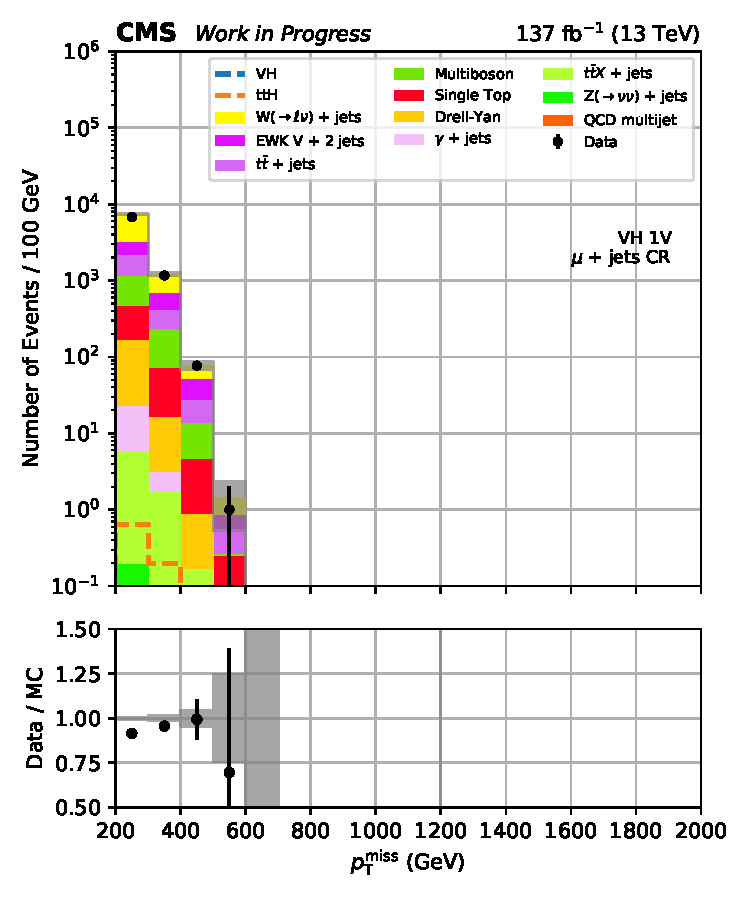
\includegraphics[width=\textwidth]{figures/region_plots/2016to18/region_1/VH_1V.pdf}
        \caption{\VH 1V}
    \end{subfigure}
    \hfill
    \begin{subfigure}[b]{0.24\textwidth}
        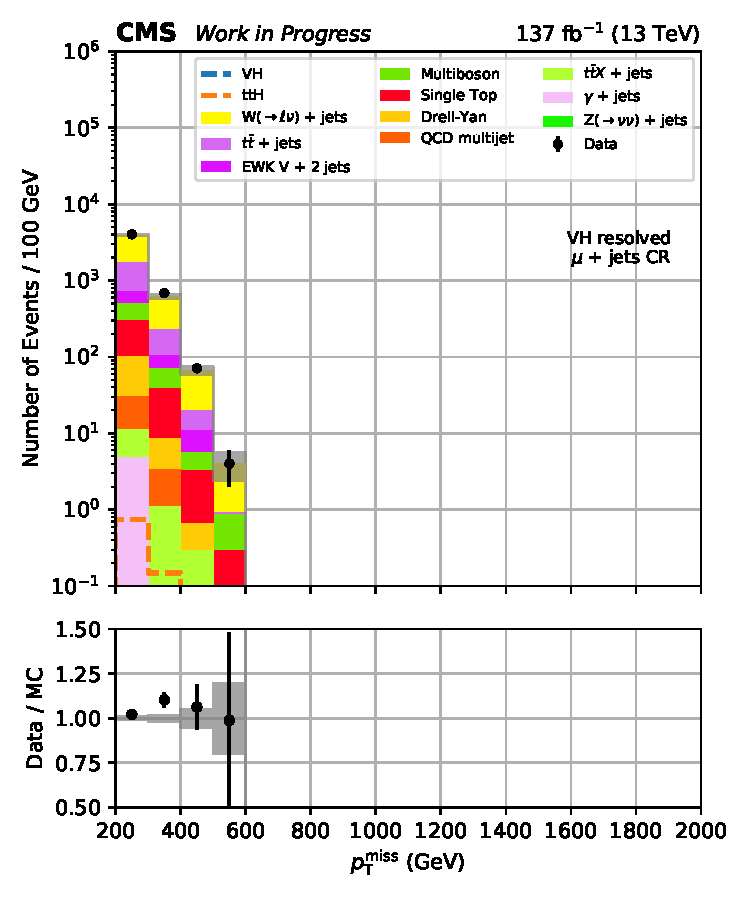
\includegraphics[width=\textwidth]{figures/region_plots/2016to18/region_1/VH_resolved.pdf}
        \caption{\VH resolved}
    \end{subfigure}
    \caption[Pre-fit yields of the \ptmiss distribution in the \singleMuCr control region for the combined boosted and resolved categories for the \ttH and \VH processes, using the full Run-2 dataset for data and simulation]{Pre-fit yields of the \ptmiss distribution in the \singleMuCr \gls{CR} for the combined boosted and resolved categories for the \ttH and \VH processes, using the full Run-2 dataset for data and simulation.}
    \label{fig:htoinv_cr_yields_comb2016to18_single_muon}
\end{figure}

\begin{figure}[htbp]
    \centering
    \begin{subfigure}[b]{0.24\textwidth}
        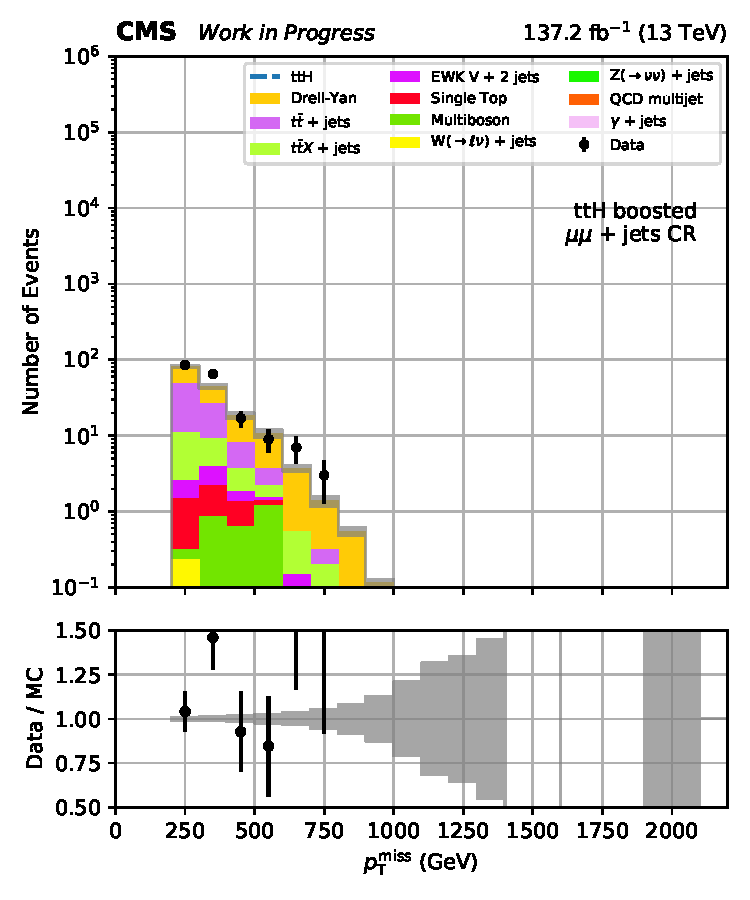
\includegraphics[width=\textwidth]{figures/region_plots/2016to18/region_2/ttH_boosted.pdf}
        \caption{\ttH boosted}
    \end{subfigure}
    \hfill
    \begin{subfigure}[b]{0.24\textwidth}
        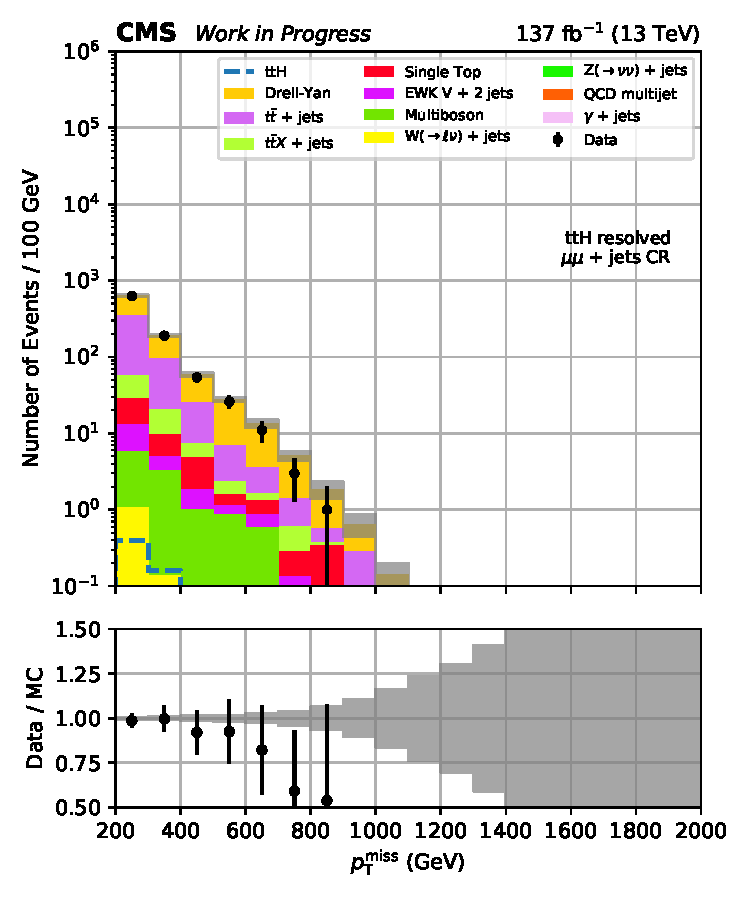
\includegraphics[width=\textwidth]{figures/region_plots/2016to18/region_2/ttH_resolved.pdf}
        \caption{\ttH resolved}
    \end{subfigure}
    \hfill
    \begin{subfigure}[b]{0.24\textwidth}
        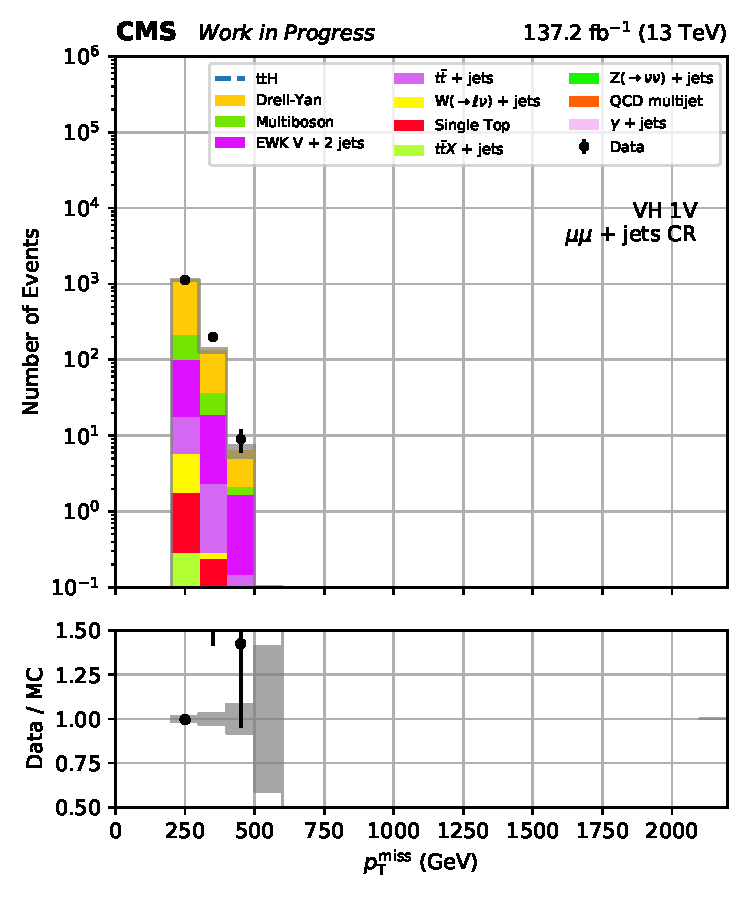
\includegraphics[width=\textwidth]{figures/region_plots/2016to18/region_2/VH_1V.pdf}
        \caption{\VH 1V}
    \end{subfigure}
    \hfill
    \begin{subfigure}[b]{0.24\textwidth}
        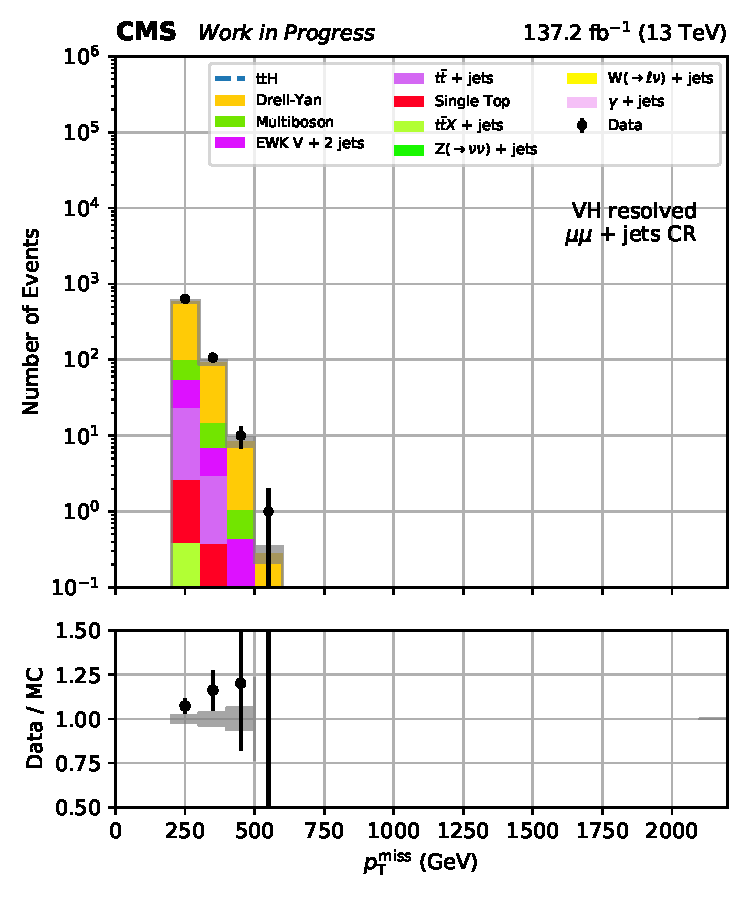
\includegraphics[width=\textwidth]{figures/region_plots/2016to18/region_2/VH_resolved.pdf}
        \caption{\VH resolved}
    \end{subfigure}
    \caption[Pre-fit yields of the \ptmiss distribution in the \doubleMuCr control region for the combined boosted and resolved categories for the \ttH and \VH processes, using the full Run-2 dataset for data and simulation]{Pre-fit yields of the \ptmiss distribution in the \doubleMuCr \gls{CR} for the combined boosted and resolved categories for the \ttH and \VH processes, using the full Run-2 dataset for data and simulation.}
    \label{fig:htoinv_cr_yields_comb2016to18_double_muon}
\end{figure}

\begin{figure}[htbp]
    \centering
    \begin{subfigure}[b]{0.24\textwidth}
        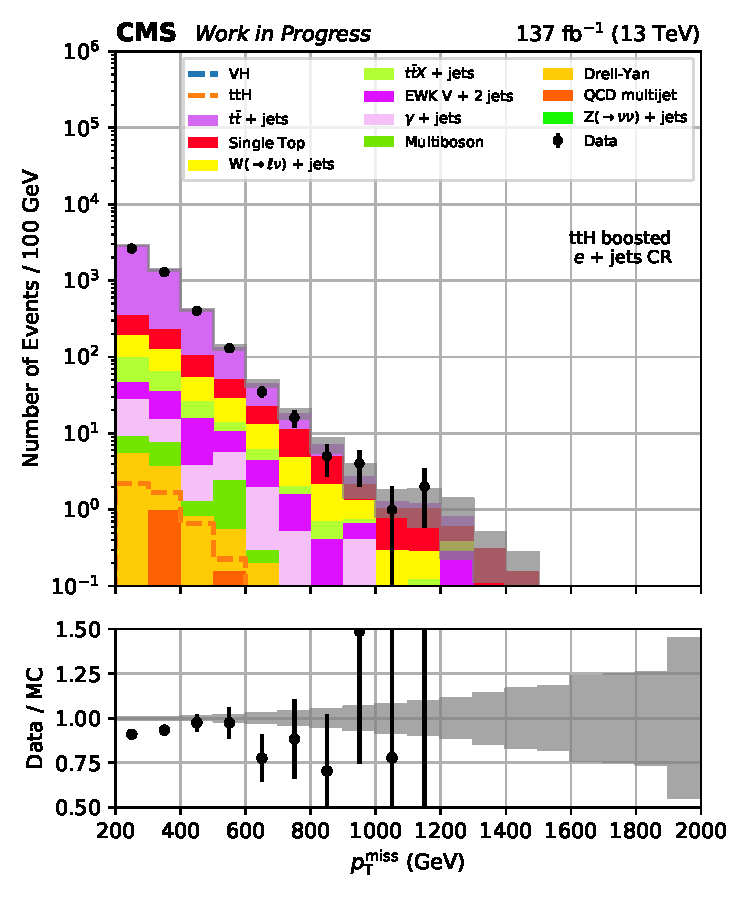
\includegraphics[width=\textwidth]{figures/region_plots/2016to18/region_3/ttH_boosted.pdf}
        \caption{\ttH boosted}
    \end{subfigure}
    \hfill
    \begin{subfigure}[b]{0.24\textwidth}
        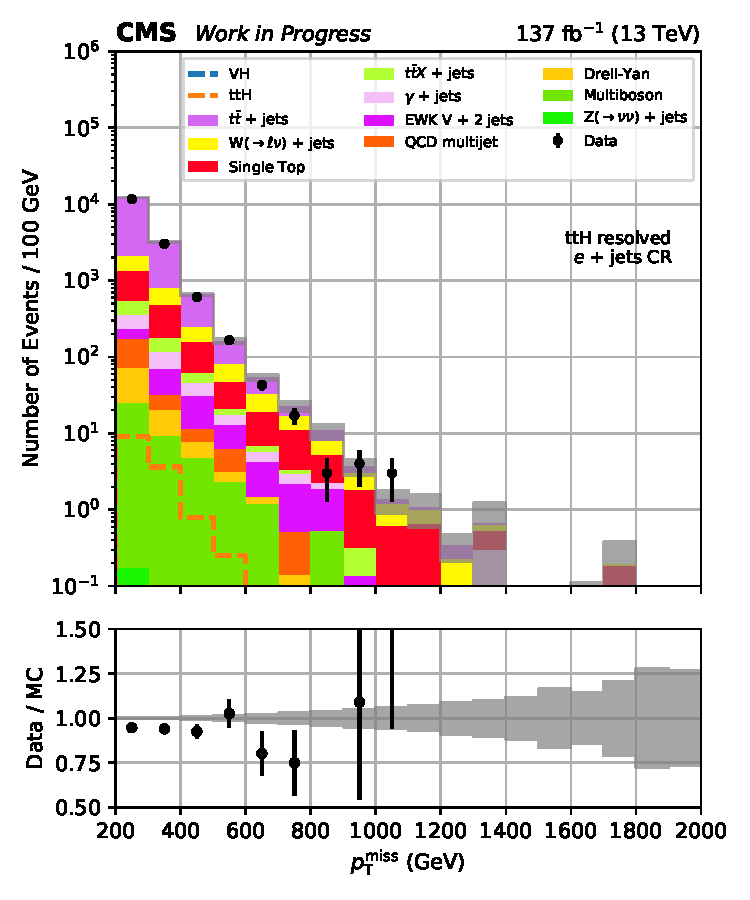
\includegraphics[width=\textwidth]{figures/region_plots/2016to18/region_3/ttH_resolved.pdf}
        \caption{\ttH resolved}
    \end{subfigure}
    \hfill
    \begin{subfigure}[b]{0.24\textwidth}
        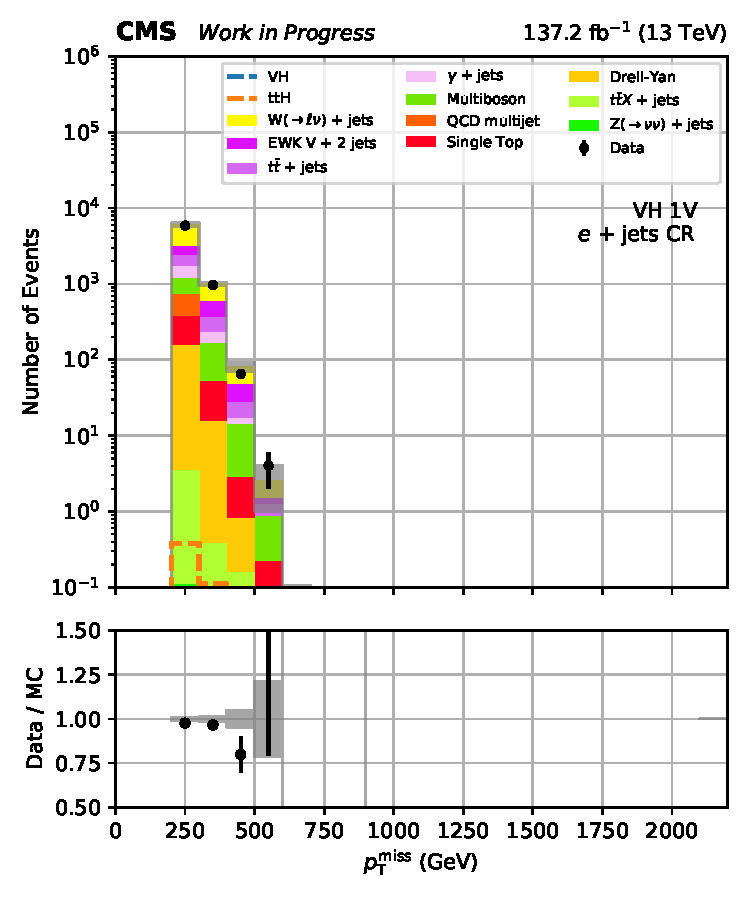
\includegraphics[width=\textwidth]{figures/region_plots/2016to18/region_3/VH_1V.pdf}
        \caption{\VH 1V}
    \end{subfigure}
    \hfill
    \begin{subfigure}[b]{0.24\textwidth}
        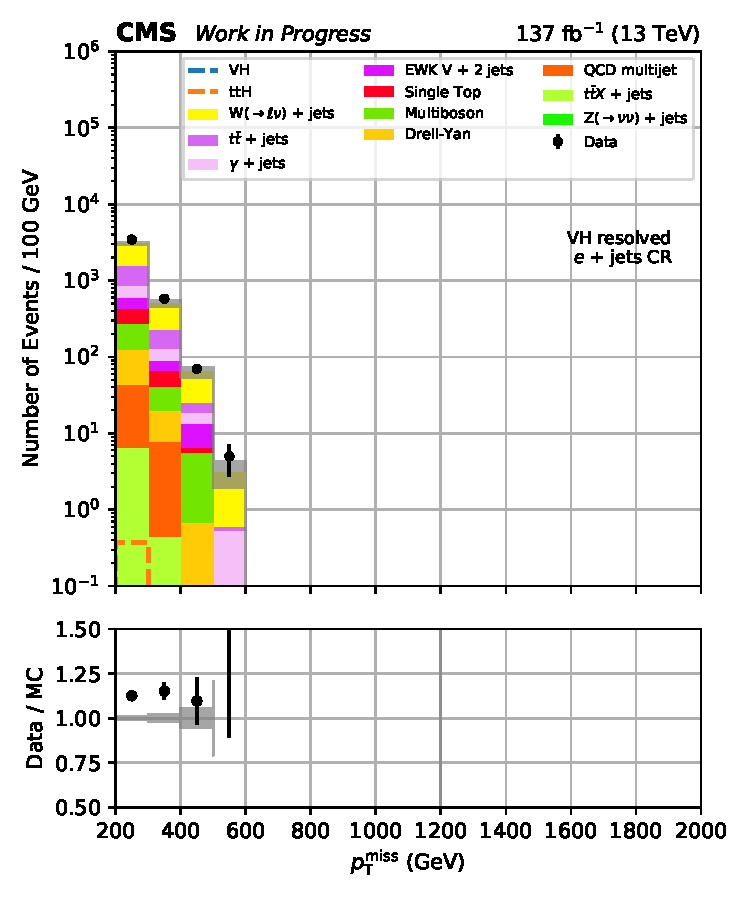
\includegraphics[width=\textwidth]{figures/region_plots/2016to18/region_3/VH_resolved.pdf}
        \caption{\VH resolved}
    \end{subfigure}
    \caption[Pre-fit yields of the \ptmiss distribution in the \singleEleCr control region for the combined boosted and resolved categories for the \ttH and \VH processes, using the full Run-2 dataset for data and simulation]{Pre-fit yields of the \ptmiss distribution in the \singleEleCr \gls{CR} for the combined boosted and resolved categories for the \ttH and \VH processes, using the full Run-2 dataset for data and simulation.}
    \label{fig:htoinv_cr_yields_comb2016to18_single_electron}
\end{figure}

\begin{figure}[htbp]
    \centering
    \begin{subfigure}[b]{0.24\textwidth}
        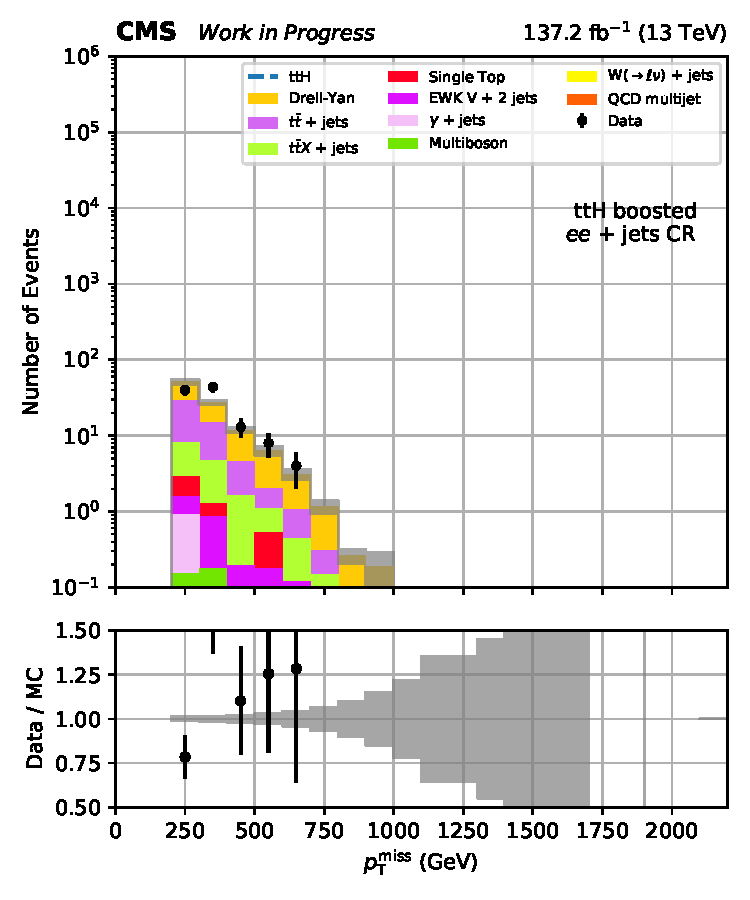
\includegraphics[width=\textwidth]{figures/region_plots/2016to18/region_4/ttH_boosted.pdf}
        \caption{\ttH boosted}
    \end{subfigure}
    \hfill
    \begin{subfigure}[b]{0.24\textwidth}
        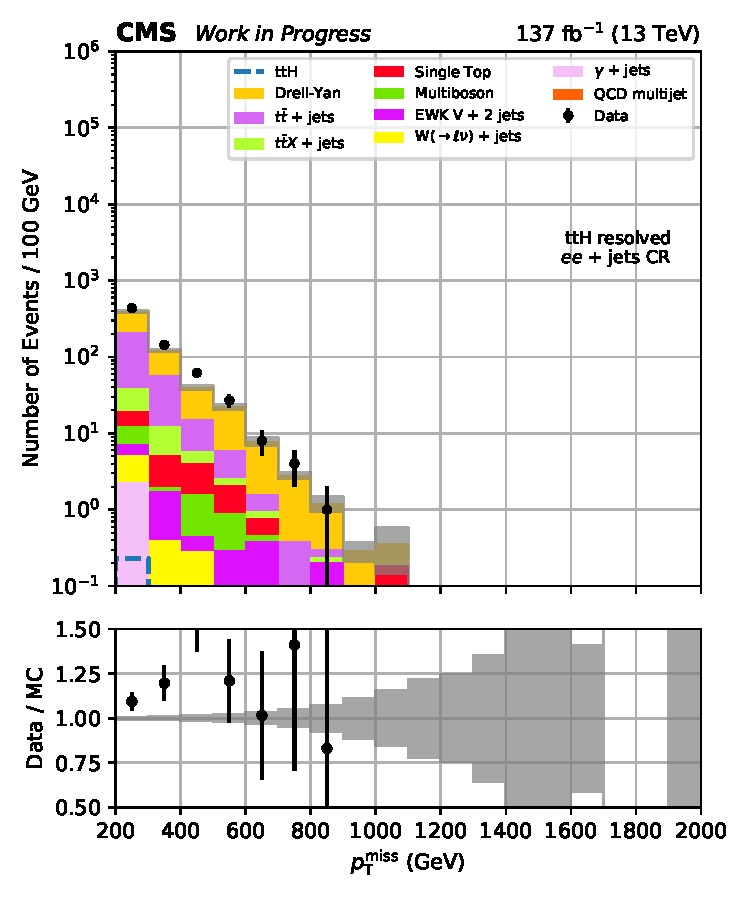
\includegraphics[width=\textwidth]{figures/region_plots/2016to18/region_4/ttH_resolved.pdf}
        \caption{\ttH resolved}
    \end{subfigure}
    \hfill
    \begin{subfigure}[b]{0.24\textwidth}
        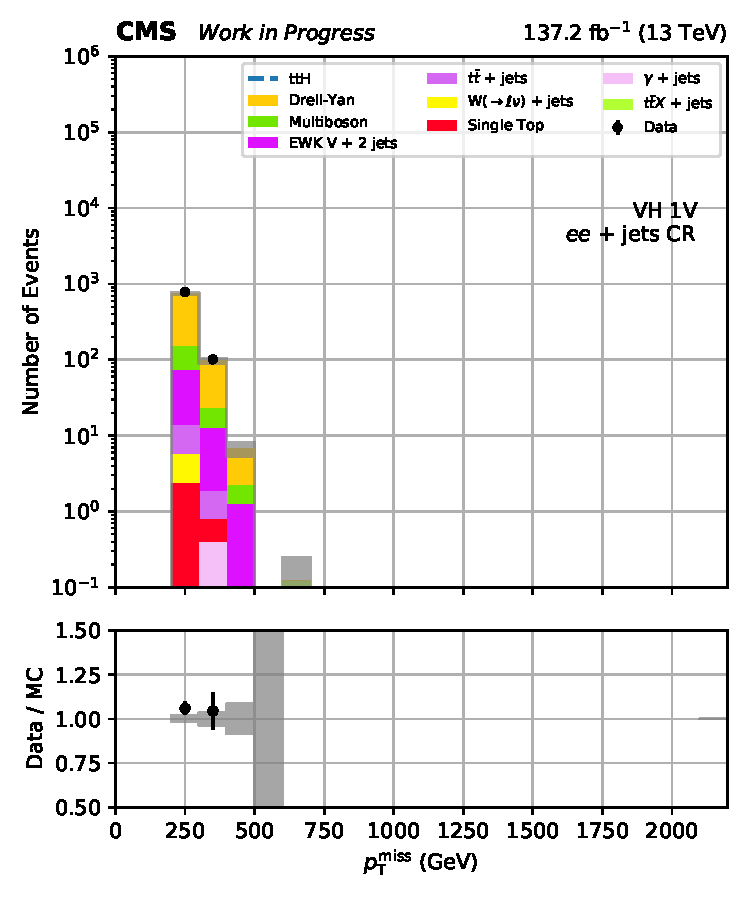
\includegraphics[width=\textwidth]{figures/region_plots/2016to18/region_4/VH_1V.pdf}
        \caption{\VH 1V}
    \end{subfigure}
    \hfill
    \begin{subfigure}[b]{0.24\textwidth}
        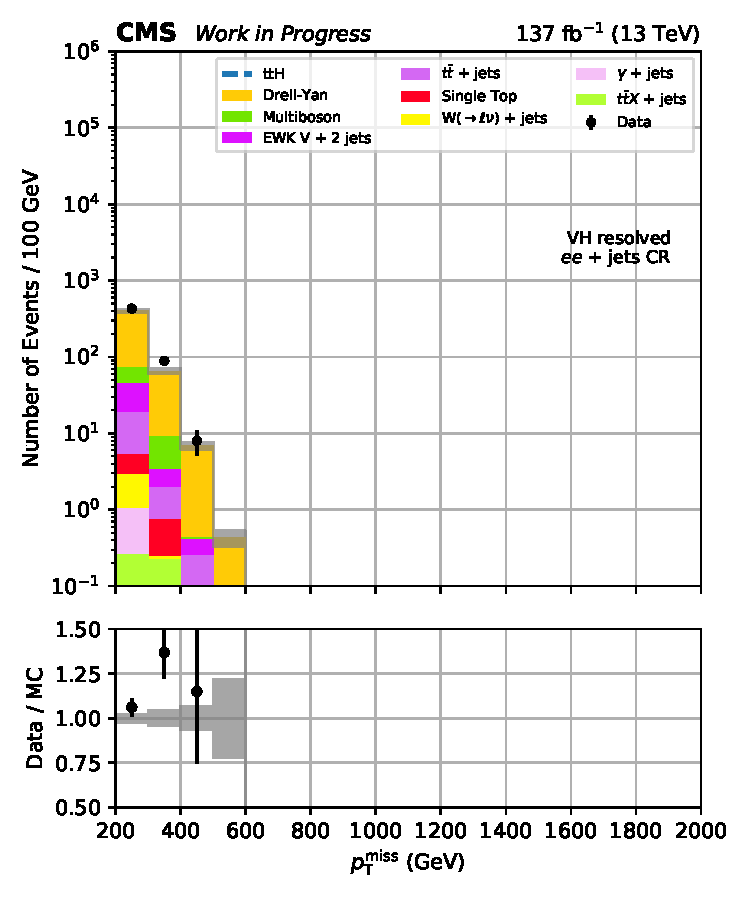
\includegraphics[width=\textwidth]{figures/region_plots/2016to18/region_4/VH_resolved.pdf}
        \caption{\VH resolved}
    \end{subfigure}
    \caption[Pre-fit yields of the \ptmiss distribution in the \doubleEleCr control region for the combined boosted and resolved categories for the \ttH and \VH processes, using the full Run-2 dataset for data and simulation]{Pre-fit yields of the \ptmiss distribution in the \doubleEleCr \gls{CR} for the combined boosted and resolved categories for the \ttH and \VH processes, using the full Run-2 dataset for data and simulation.}
    \label{fig:htoinv_cr_yields_comb2016to18_double_electron}
\end{figure}

\begin{figure}[htbp]
    \centering
    \begin{subfigure}[b]{0.24\textwidth}
        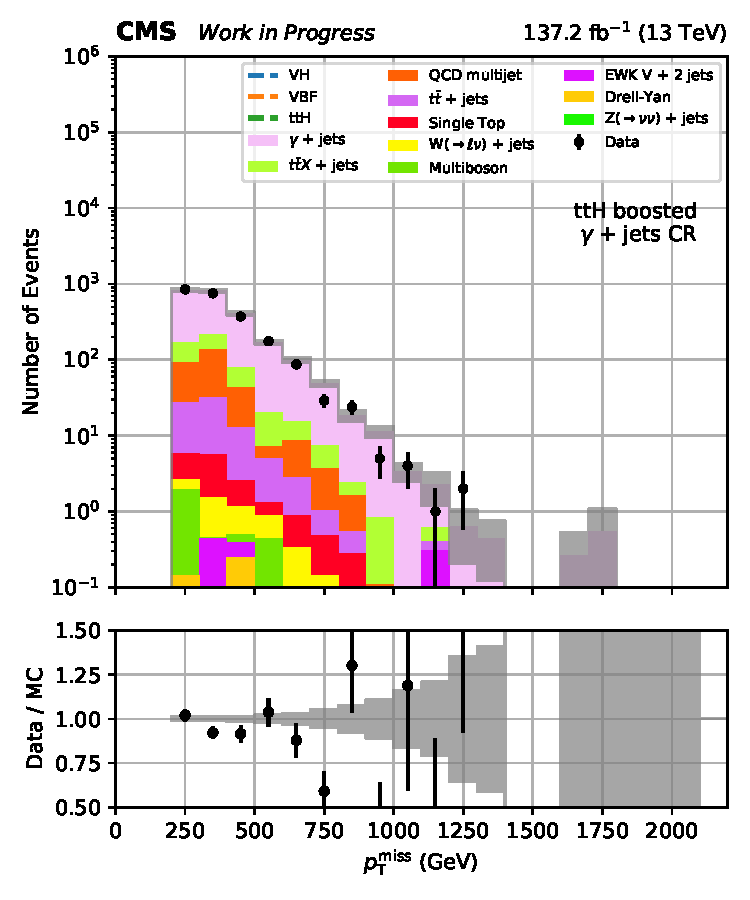
\includegraphics[width=\textwidth]{figures/region_plots/2016to18/region_5/ttH_boosted.pdf}
        \caption{\ttH boosted}
    \end{subfigure}
    \hfill
    \begin{subfigure}[b]{0.24\textwidth}
        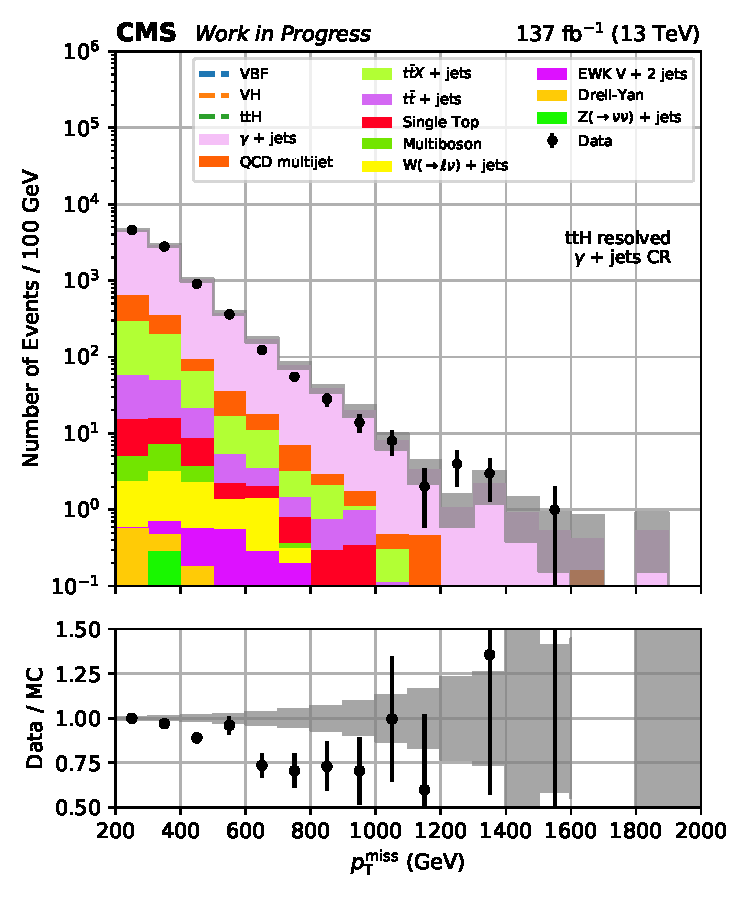
\includegraphics[width=\textwidth]{figures/region_plots/2016to18/region_5/ttH_resolved.pdf}
        \caption{\ttH resolved}
    \end{subfigure}
    \hfill
    \begin{subfigure}[b]{0.24\textwidth}
        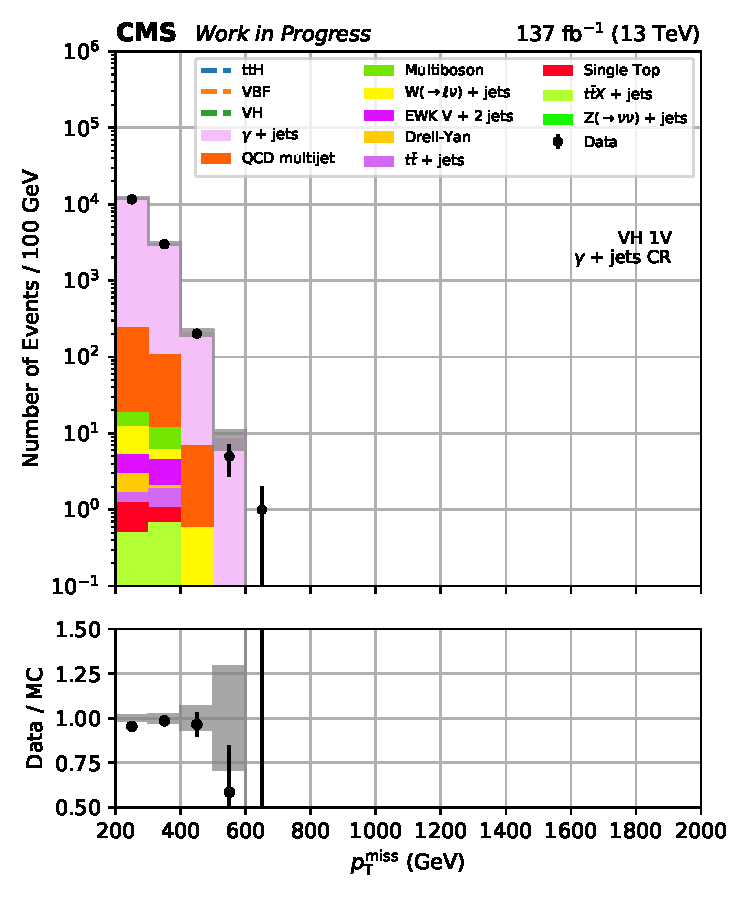
\includegraphics[width=\textwidth]{figures/region_plots/2016to18/region_5/VH_1V.pdf}
        \caption{\VH 1V}
    \end{subfigure}
    \hfill
    \begin{subfigure}[b]{0.24\textwidth}
        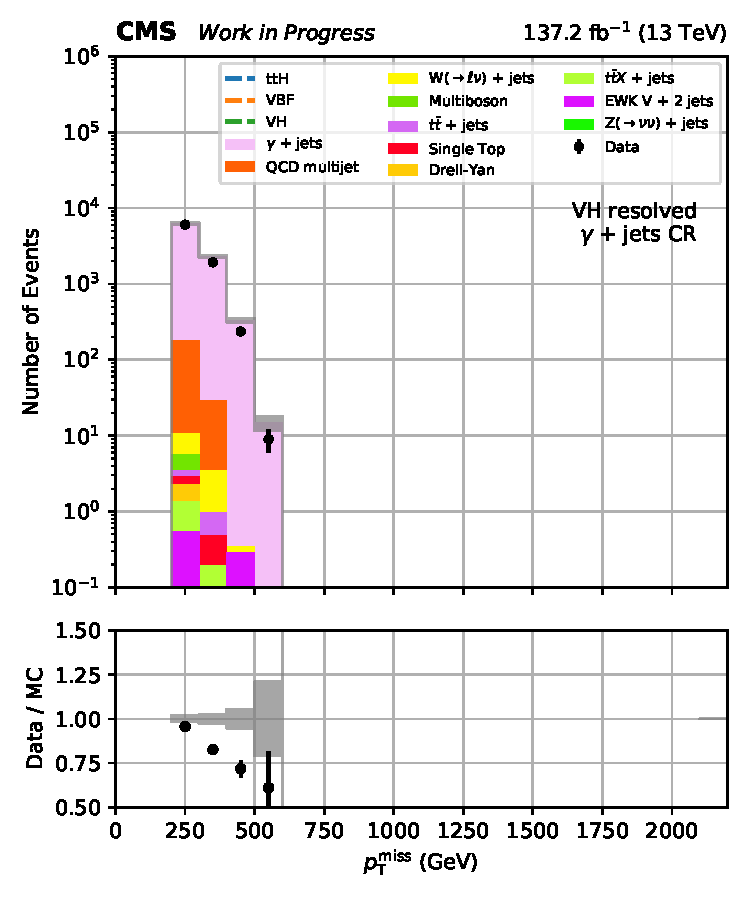
\includegraphics[width=\textwidth]{figures/region_plots/2016to18/region_5/VH_resolved.pdf}
        \caption{\VH resolved}
    \end{subfigure}
    \caption[Pre-fit yields of the \ptmiss distribution in the \singlePhotonCr control region for the combined boosted and resolved categories for the \ttH and \VH processes, using the full Run-2 dataset for data and simulation]{Pre-fit yields of the \ptmiss distribution in the \singlePhotonCr \gls{CR} for the combined boosted and resolved categories for the \ttH and \VH processes, using the full Run-2 dataset for data and simulation. The \singlePhotonCr is more useful in predicting \ztonunupjets in the \VH subcategories, and may not be used for the \ttH subcategories.}
    \label{fig:htoinv_cr_yields_comb2016to18_single_photon}
\end{figure}

% Figures from 29th May, 2020


%=========================================================


\subsection{Sidebands to the signal region}
\label{subsec:htoinv_sidebands}

As explained in Chpt.~\ref{subsec:htoinv_background}, it is difficult to accurately estimate the \acrshort{qcd} multijet content in the signal region. Several kinematic cuts in the analysis are designed to reject \acrshort{qcd} in the signal region, so by inverting one or two of them, we can construct multijet-enriched regions: \emph{\glspl{SB}}.

We invert the requirements on $\mht/\ptmiss$---where a ceiling is placed at $\mht/\ptmiss = 4$ to reject severely-mismeasured \glspl{jet}---and the angular variable designed to optimise the categorisation of the production modes (see Chpt.~\ref{subsec:htoinv_cat_optimisation}). Several \glspl{SB} are constructed where each cut is inverted separately, and then when both are inverted. When the angular cut is inverted, the remaining phase space may be split into two \glspl{SB}, dubbed ``loose'' and ``tight''. These are summarised for the different categories in Tabs.~\ref{tab:sidebanddefs_ttH_VH}, \ref{tab:sidebanddefs_ggF}, and \ref{tab:sidebanddefs_monojet}.

\begin{table}[htbp]
    \centering
    \begin{tabular}{c|c|c|c}
        & $\omegaTilde < 0.2$ & $0.2 \leq \omegaTilde \leq 0.5$ & $\omegaTilde > 0.5$ \\\hline
        $\mht/\ptmiss < 1.2$ & ``Tight'' \omegaTilde SB & ``Loose'' \omegaTilde SB & Signal region \\\hline
        $1.2 \leq \mht/\ptmiss < 4$ & ``Tight'' double SB & ``Loose'' double SB & $\mht/\ptmiss$ SB \\
    \end{tabular}
    \caption[Definitions of the data sidebands used to determine the QCD multijet background in the signal region for the \ttH and \VH categories]{Definitions of the \glspl{SB} (SBs) used to determine the \acrshort{qcd} multijet background in the signal region for the \ttH and \VH categories.}
    \label{tab:sidebanddefs_ttH_VH}
\end{table}

\begin{table}[htbp]
    \centering
    \begin{tabular}{c|c|c|c}
        & $\omegaTilde < 0.2$ & $0.2 \leq \omegaTilde \leq 0.7$ & $\omegaTilde > 0.7$ \\\hline
        $\mht/\ptmiss < 1.2$ & ``Tight'' \omegaTilde SB & ``Loose'' \omegaTilde SB & Signal region \\\hline
        $1.2 \leq \mht/\ptmiss < 4$ & ``Tight'' double SB & ``Loose'' double SB & $\mht/\ptmiss$ SB \\
    \end{tabular}
    \caption[Definitions of the data sidebands used to determine the QCD multijet background in the signal region for the \ggH categories]{Definitions of the \glspl{SB} (SBs) used to determine the \acrshort{qcd} multijet background in the signal region for the \ggH categories.}
    \label{tab:sidebanddefs_ggF}
\end{table}

\begin{table}[htbp]
    \centering
    \begin{tabular}{c|c|c}
        & $0.1 \leq \dphiFj \leq 2.5$ & $\dphiFj > 2.5$ \\\hline
        $\mht/\ptmiss < 1.2$ & \dphiFj sideband & Signal region \\\hline
        $1.2 \leq \mht/\ptmiss < 4$ & Double sideband & $\mht/\ptmiss$ sideband \\
    \end{tabular}
    \caption[Definitions of the data sidebands used to determine the QCD multijet background in the signal region for the monojet categories]{Definitions of the \glspl{SB} used to determine the \acrshort{qcd} multijet background in the signal region for the monojet categories.}
    \label{tab:sidebanddefs_monojet}
\end{table}

% Wrap the numbers in the tables above in \text{}, once they're finalised

The \glspl{SB} follow the same categorisation as for the other regions, i.e., Tab.~\ref{tab:htoinv_categories}, and are binned in \ptmiss with the same scheme as the other regions.

A \gls{SB} composed of the inversion of only one variable maintains similar kinematic properties to the signal region. When performing analysis while still blind to data in the signal region, inspecting one of these \glspl{SB} is a good indicator of how new cuts or corrections will affect the signal region composition, and compatibility between data and \acrshort{mc}. Like the \glspl{CR}, \glspl{SB} serve a secondary purpose.

The following figures reveal the pre-fit \ptmiss distributions in each \gls{SB} after the analysis-level selections with the full Run-2 dataset. The combined \ttH and \VH subcategories for boosted and resolved topologies are used to demonstrate the shapes and data--simulation (dis)agreement. Background estimation is performed separately for each year due to the differing running conditions, detector configuration, and the different effects or problems seen in the data.\footnote{Might not need to show all of these plots. They're just here for now, and can be tidied up later.}

\begin{figure}[htbp]
    \centering
    \begin{subfigure}[b]{0.24\textwidth}
        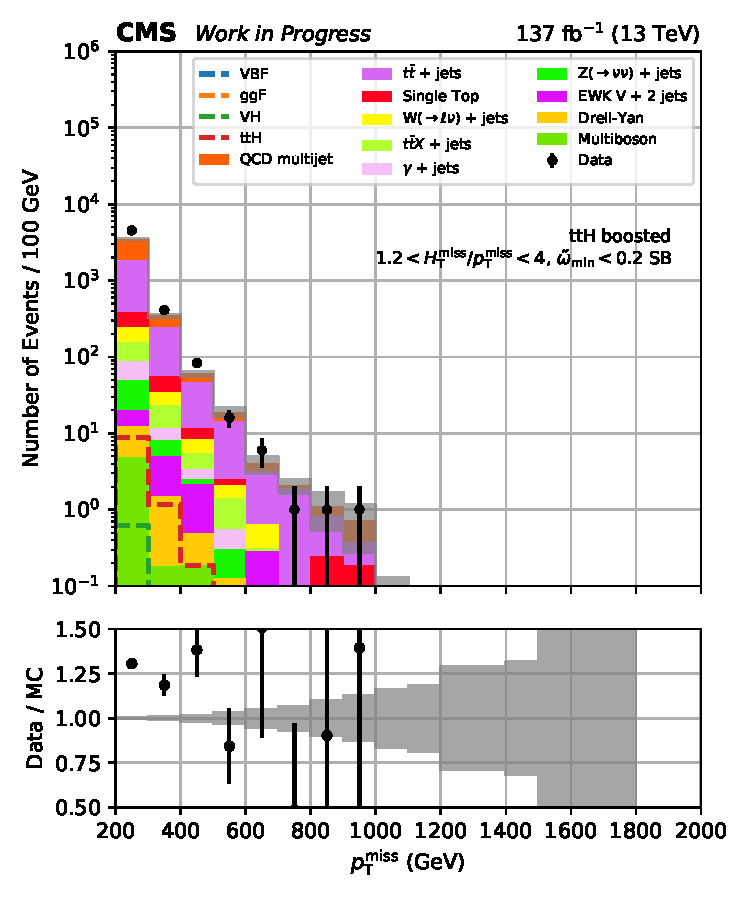
\includegraphics[width=\textwidth]{figures/region_plots/2016to18/sideband_0/ttH_boosted.pdf}
        \caption{\ttH boosted}
    \end{subfigure}
    \hfill
    \begin{subfigure}[b]{0.24\textwidth}
        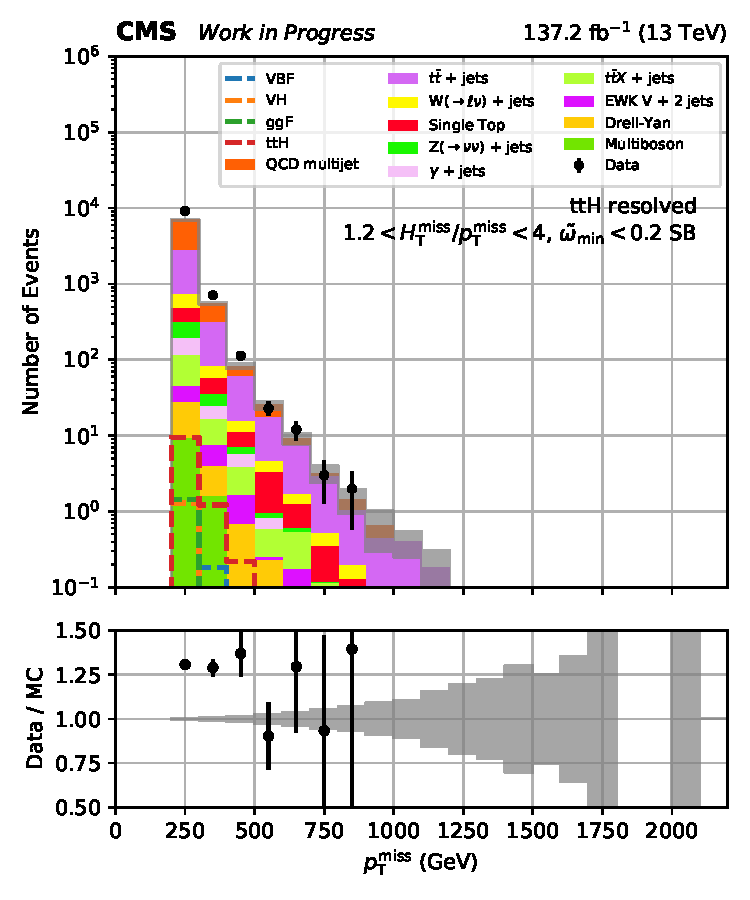
\includegraphics[width=\textwidth]{figures/region_plots/2016to18/sideband_0/ttH_resolved.pdf}
        \caption{\ttH resolved}
    \end{subfigure}
    \hfill
    \begin{subfigure}[b]{0.24\textwidth}
        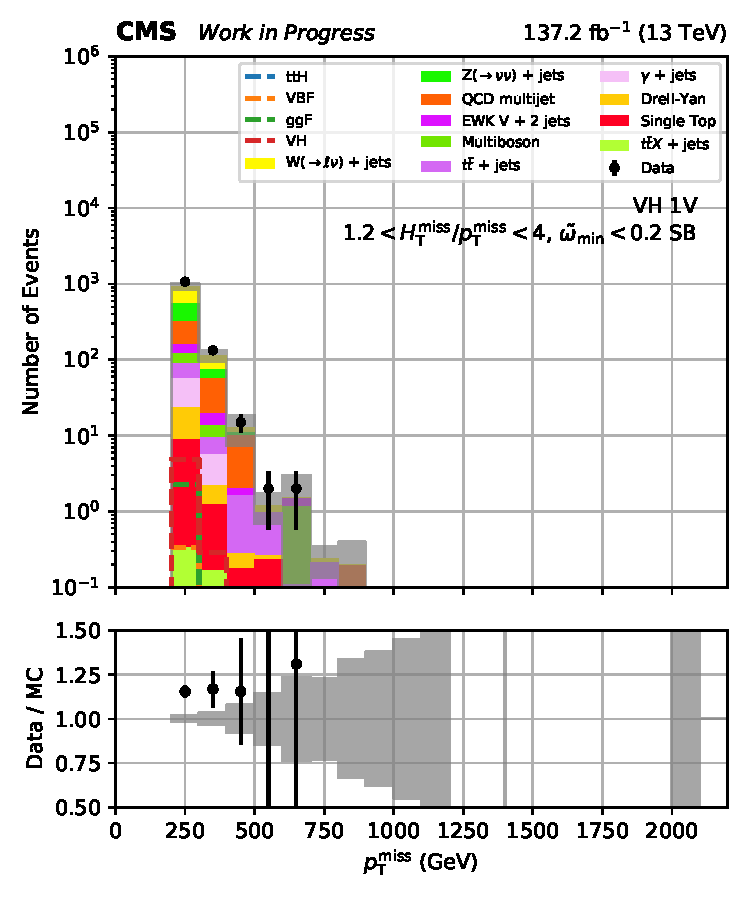
\includegraphics[width=\textwidth]{figures/region_plots/2016to18/sideband_0/VH_1V.pdf}
        \caption{\VH 1V}
    \end{subfigure}
    \hfill
    \begin{subfigure}[b]{0.24\textwidth}
        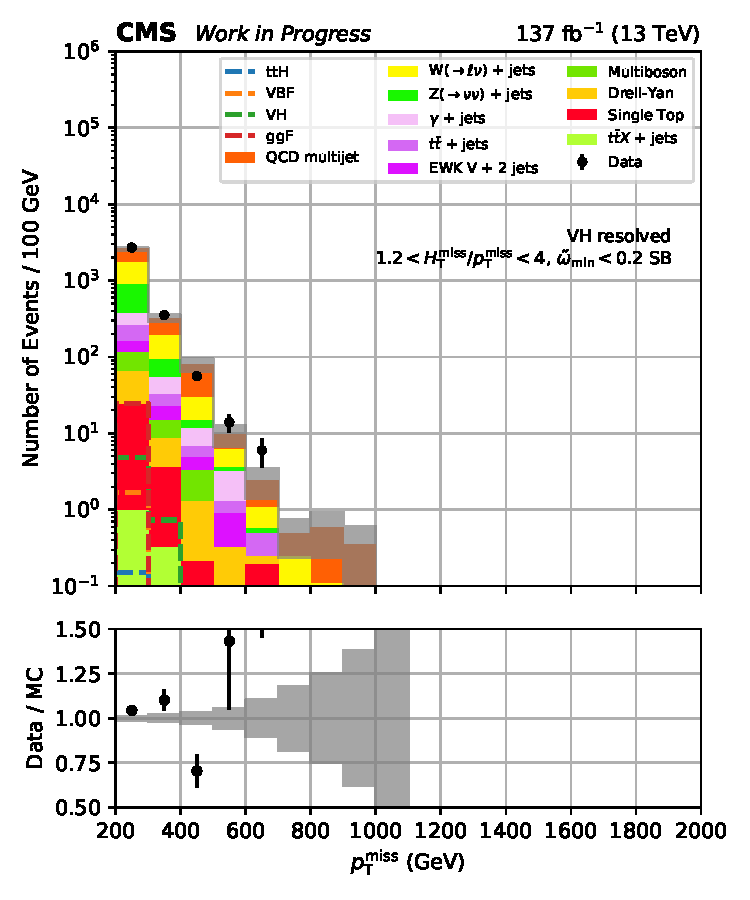
\includegraphics[width=\textwidth]{figures/region_plots/2016to18/sideband_0/VH_resolved.pdf}
        \caption{\VH resolved}
    \end{subfigure}
    \caption[Pre-fit yields of the \ptmiss distribution in the tight double sideband for the combined boosted and resolved categories for the \ttH and \VH processes, using the full Run-2 dataset for data and simulation]{Pre-fit yields of the \ptmiss distribution in the tight double \gls{SB} for the combined boosted and resolved categories for the \ttH and \VH processes, using the full Run-2 dataset for data and simulation.}
    \label{fig:htoinv_sb_yields_comb2016to18_tight_double}
\end{figure}

\begin{figure}[htbp]
    \centering
    \begin{subfigure}[b]{0.24\textwidth}
        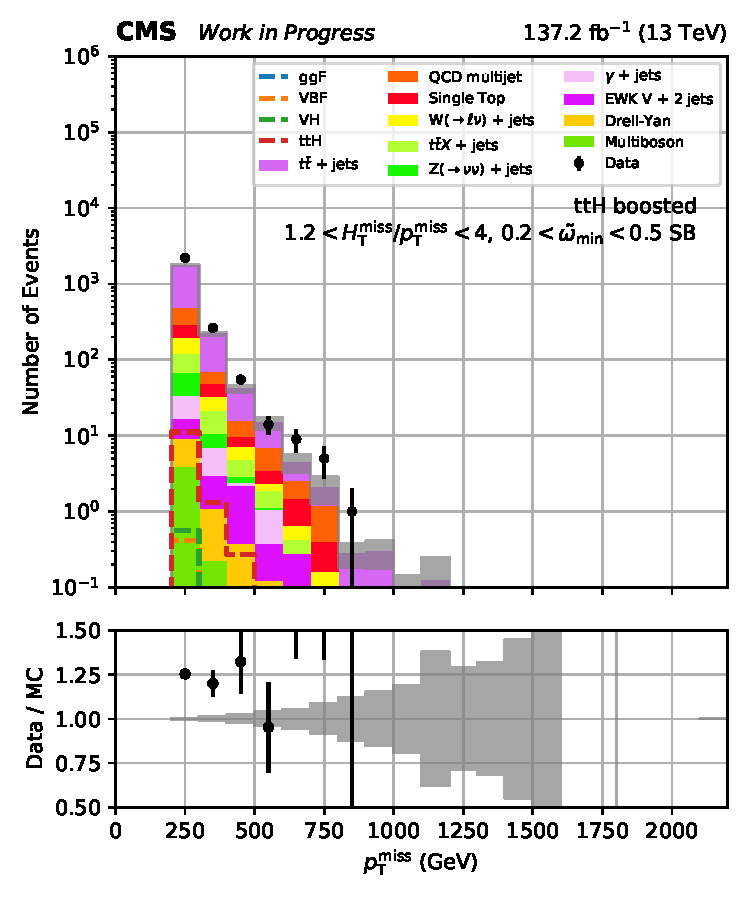
\includegraphics[width=\textwidth]{figures/region_plots/2016to18/sideband_1/ttH_boosted.pdf}
        \caption{\ttH boosted}
    \end{subfigure}
    \hfill
    \begin{subfigure}[b]{0.24\textwidth}
        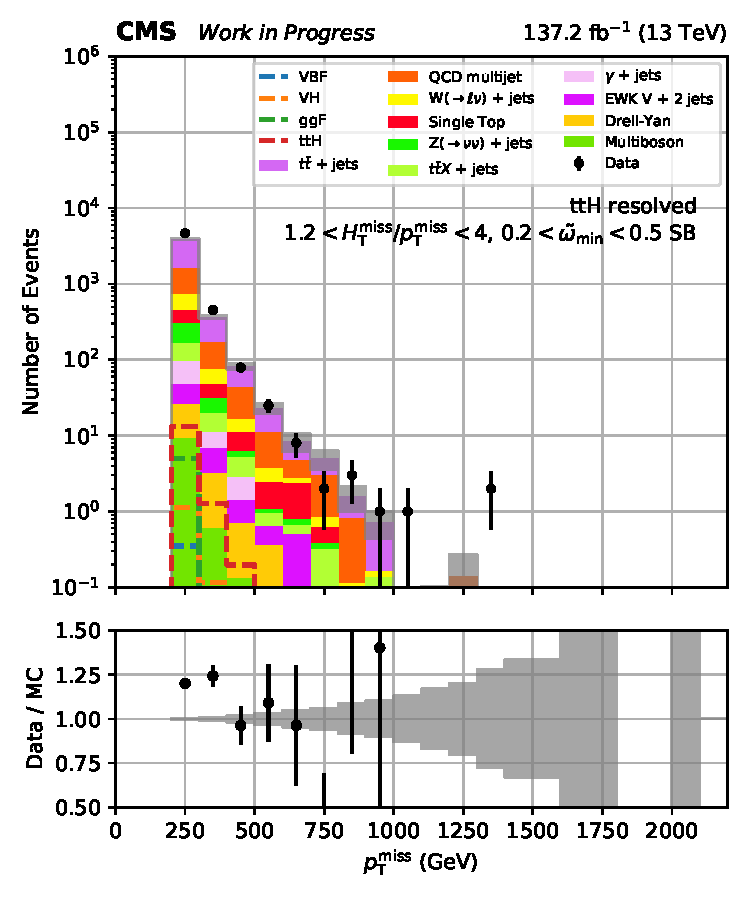
\includegraphics[width=\textwidth]{figures/region_plots/2016to18/sideband_1/ttH_resolved.pdf}
        \caption{\ttH resolved}
    \end{subfigure}
    \hfill
    \begin{subfigure}[b]{0.24\textwidth}
        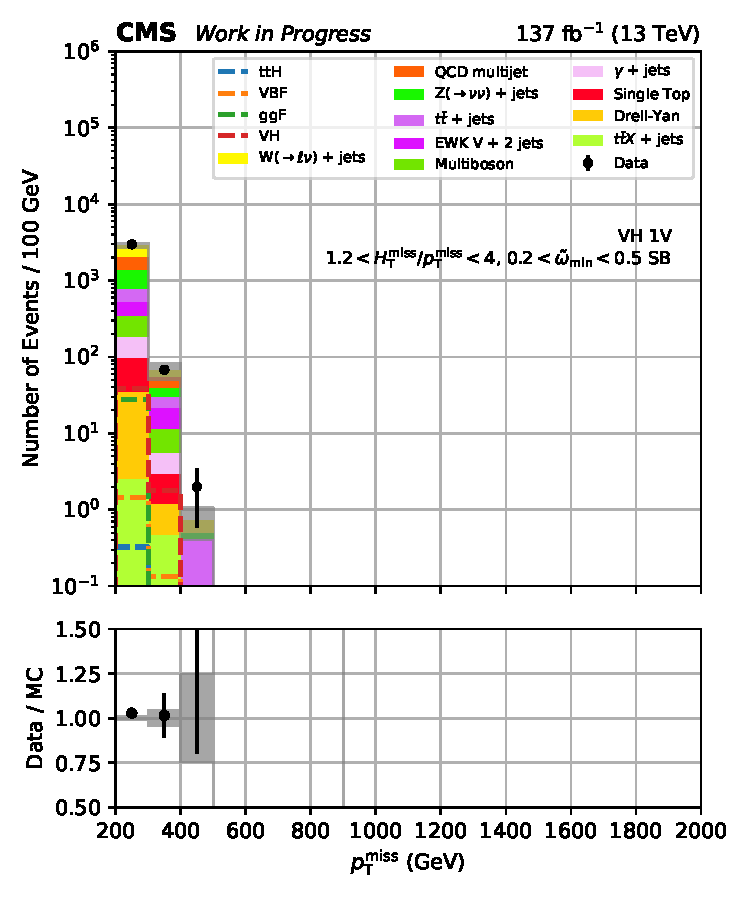
\includegraphics[width=\textwidth]{figures/region_plots/2016to18/sideband_1/VH_1V.pdf}
        \caption{\VH 1V}
    \end{subfigure}
    \hfill
    \begin{subfigure}[b]{0.24\textwidth}
        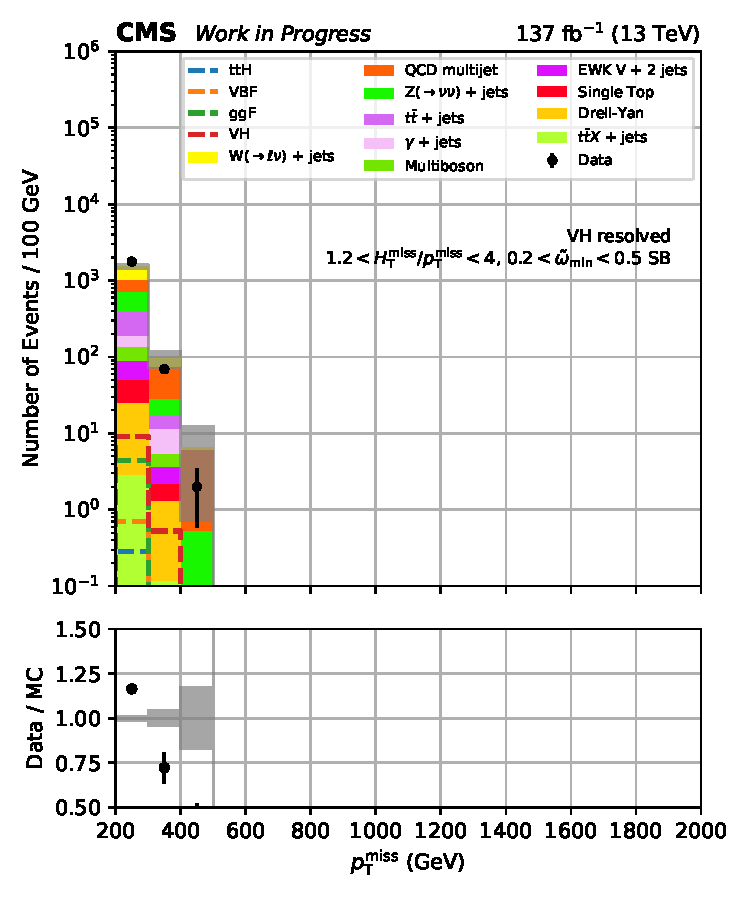
\includegraphics[width=\textwidth]{figures/region_plots/2016to18/sideband_1/VH_resolved.pdf}
        \caption{\VH resolved}
    \end{subfigure}
    \caption[Pre-fit yields of the \ptmiss distribution in the loose double sideband for the combined boosted and resolved categories for the \ttH and \VH processes, using the full Run-2 dataset for data and simulation]{Pre-fit yields of the \ptmiss distribution in the loose double \gls{SB} for the combined boosted and resolved categories for the \ttH and \VH processes, using the full Run-2 dataset for data and simulation.}
    \label{fig:htoinv_sb_yields_comb2016to18_loose_double}
\end{figure}
\begin{figure}[htbp]
    \centering
    \begin{subfigure}[b]{0.24\textwidth}
        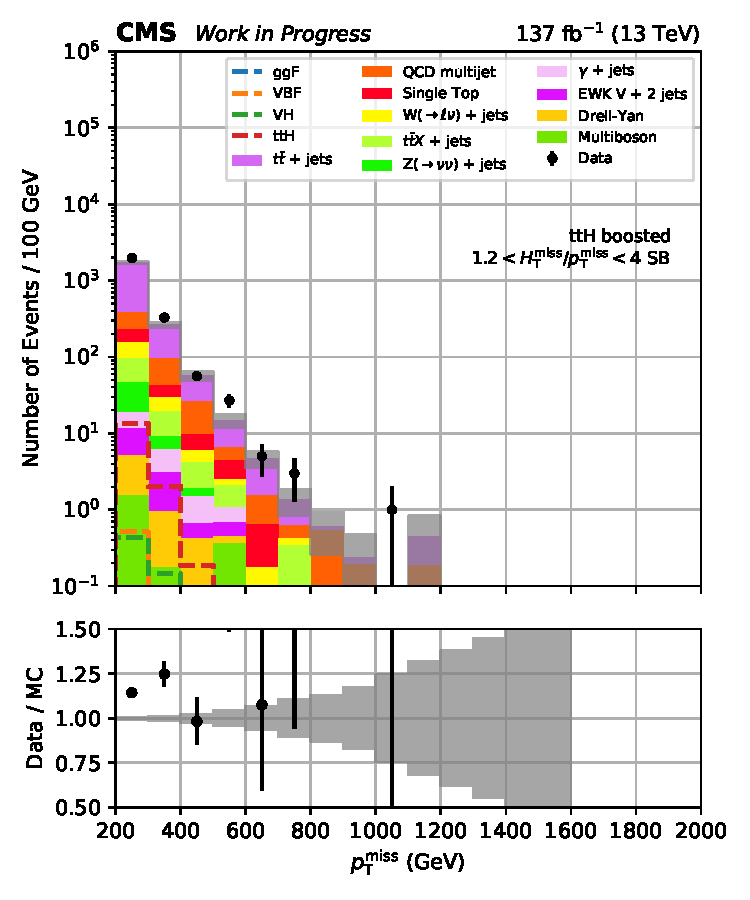
\includegraphics[width=\textwidth]{figures/region_plots/2016to18/sideband_2/ttH_boosted.pdf}
        \caption{\ttH boosted}
    \end{subfigure}
    \hfill
    \begin{subfigure}[b]{0.24\textwidth}
        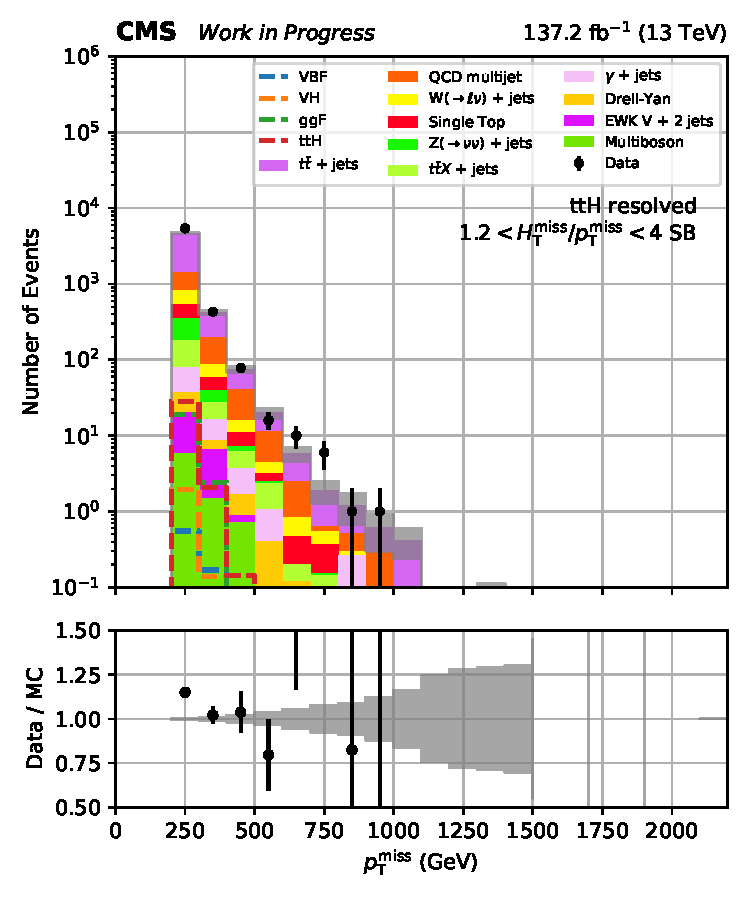
\includegraphics[width=\textwidth]{figures/region_plots/2016to18/sideband_2/ttH_resolved.pdf}
        \caption{\ttH resolved}
    \end{subfigure}
    \hfill
    \begin{subfigure}[b]{0.24\textwidth}
        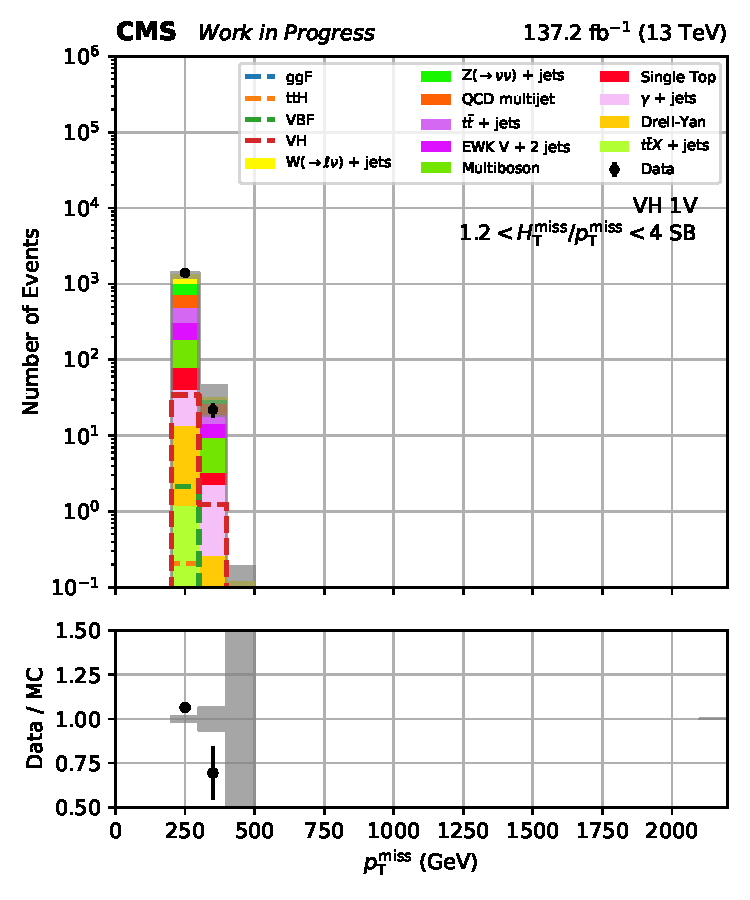
\includegraphics[width=\textwidth]{figures/region_plots/2016to18/sideband_2/VH_1V.pdf}
        \caption{\VH 1V}
    \end{subfigure}
    \hfill
    \begin{subfigure}[b]{0.24\textwidth}
        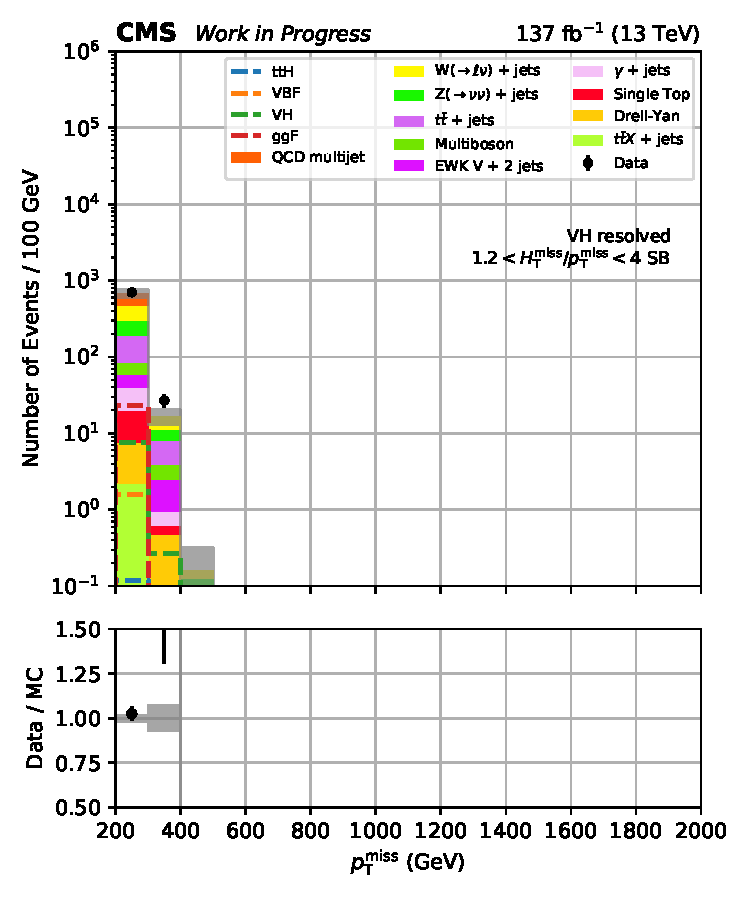
\includegraphics[width=\textwidth]{figures/region_plots/2016to18/sideband_2/VH_resolved.pdf}
        \caption{\VH resolved}
    \end{subfigure}
    \caption[Pre-fit yields of the \ptmiss distribution in the $\mht/\ptmiss$ sideband for the combined boosted and resolved categories for the \ttH and \VH processes, using the full Run-2 dataset for data and simulation]{Pre-fit yields of the \ptmiss distribution in the $\mht/\ptmiss$ \gls{SB} for the combined boosted and resolved categories for the \ttH and \VH processes, using the full Run-2 dataset for data and simulation.}
    \label{fig:htoinv_sb_yields_comb2016to18_mht_met}
\end{figure}

\begin{figure}[htbp]
    \centering
    \begin{subfigure}[b]{0.24\textwidth}
        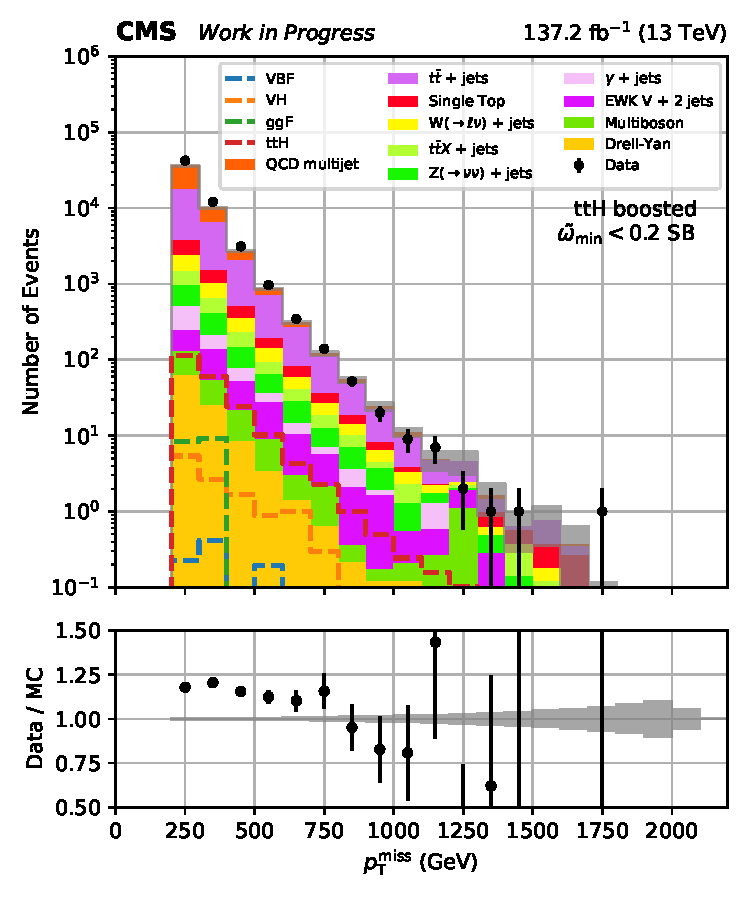
\includegraphics[width=\textwidth]{figures/region_plots/2016to18/sideband_3/ttH_boosted.pdf}
        \caption{\ttH boosted}
    \end{subfigure}
    \hfill
    \begin{subfigure}[b]{0.24\textwidth}
        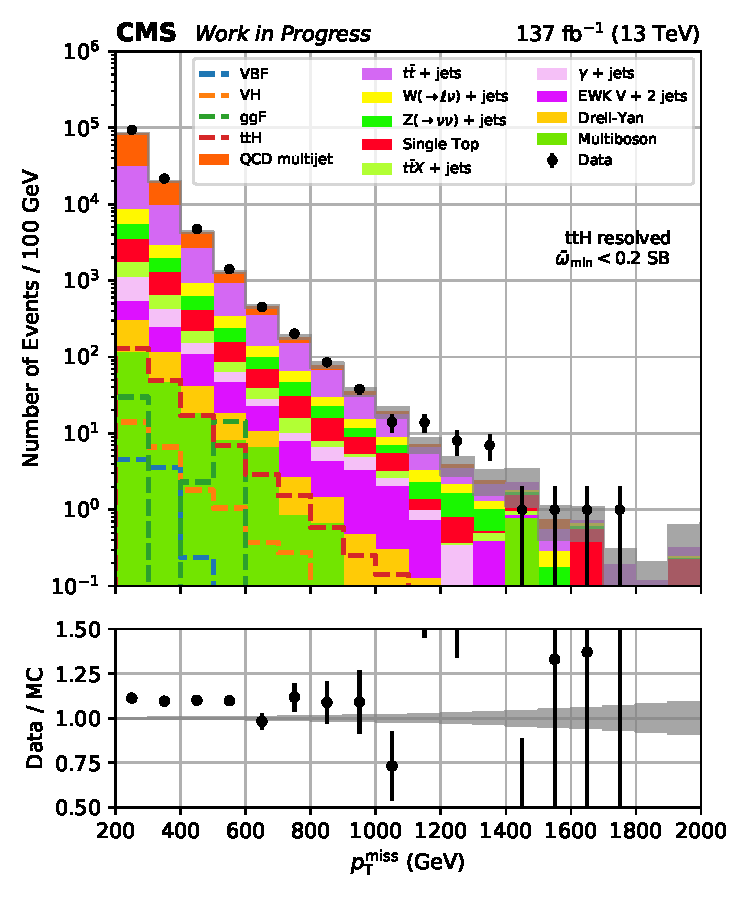
\includegraphics[width=\textwidth]{figures/region_plots/2016to18/sideband_3/ttH_resolved.pdf}
        \caption{\ttH resolved}
    \end{subfigure}
    \hfill
    \begin{subfigure}[b]{0.24\textwidth}
        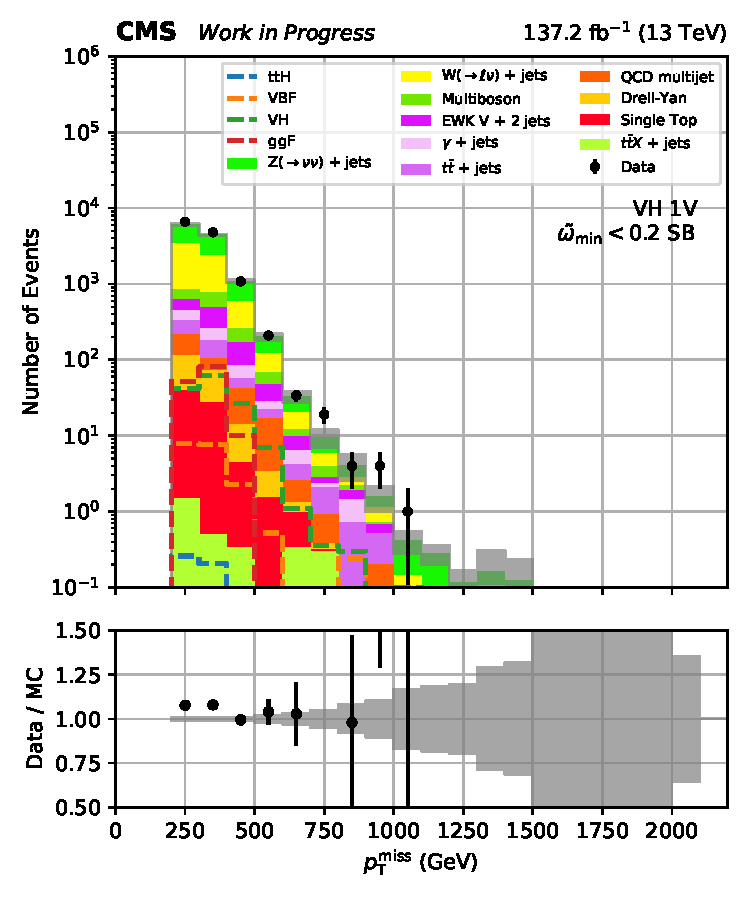
\includegraphics[width=\textwidth]{figures/region_plots/2016to18/sideband_3/VH_1V.pdf}
        \caption{\VH 1V}
    \end{subfigure}
    \hfill
    \begin{subfigure}[b]{0.24\textwidth}
        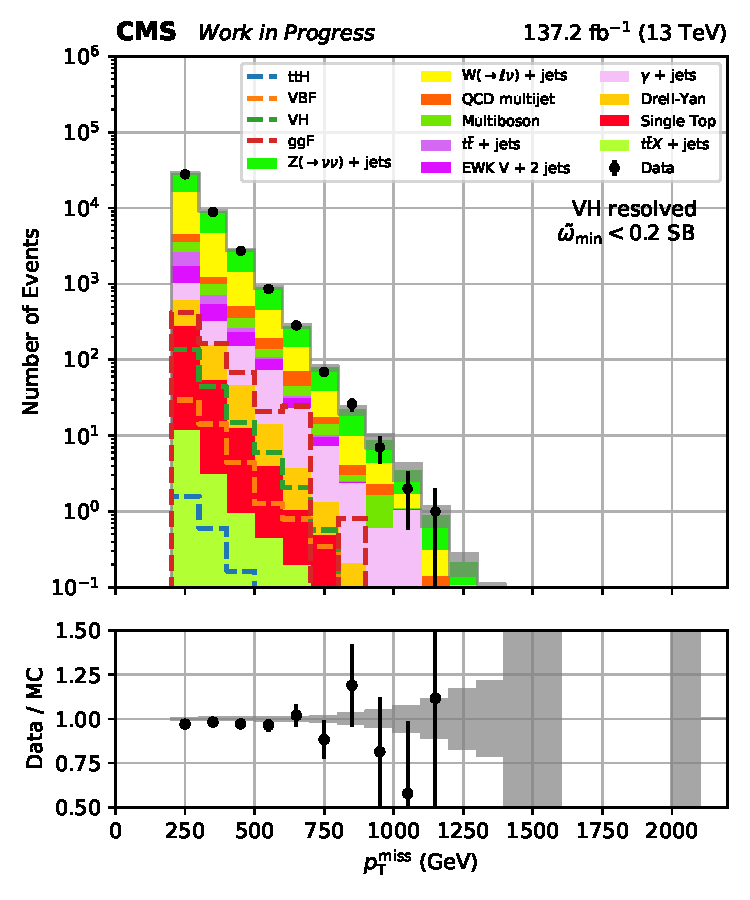
\includegraphics[width=\textwidth]{figures/region_plots/2016to18/sideband_3/VH_resolved.pdf}
        \caption{\VH resolved}
    \end{subfigure}
    \caption[Pre-fit yields of the \ptmiss distribution in the tight \omegaTilde sideband for the combined boosted and resolved categories for the \ttH and \VH processes, using the full Run-2 dataset for data and simulation]{Pre-fit yields of the \ptmiss distribution in the tight \omegaTilde \gls{SB} for the combined boosted and resolved categories for the \ttH and \VH processes, using the full Run-2 dataset for data and simulation.}
    \label{fig:htoinv_sb_yields_comb2016to18_tight_minOmegaTilde}
\end{figure}

\begin{figure}[htbp]
    \centering
    \begin{subfigure}[b]{0.24\textwidth}
        \includegraphics[width=\textwidth]{figures/region_plots/2016to18/sideband_4/ttH_boosted.pdf}
        \caption{\ttH boosted}
    \end{subfigure}
    \hfill
    \begin{subfigure}[b]{0.24\textwidth}
        \includegraphics[width=\textwidth]{figures/region_plots/2016to18/sideband_4/ttH_resolved.pdf}
        \caption{\ttH resolved}
    \end{subfigure}
    \begin{subfigure}[b]{0.24\textwidth}
        \includegraphics[width=\textwidth]{figures/region_plots/2016to18/sideband_4/VH_1V.pdf}
        \caption{\VH 1V}
    \end{subfigure}
    \hfill
    \begin{subfigure}[b]{0.24\textwidth}
        \includegraphics[width=\textwidth]{figures/region_plots/2016to18/sideband_4/VH_resolved.pdf}
        \caption{\VH resolved}
    \end{subfigure}
    \caption[Pre-fit yields of the \ptmiss distribution in the loose \omegaTilde sideband for the combined boosted and resolved categories for the \ttH and \VH processes, using the full Run-2 dataset for data and simulation]{Pre-fit yields of the \ptmiss distribution in the loose \omegaTilde \gls{SB} for the combined boosted and resolved categories for the \ttH and \VH processes, using the full Run-2 dataset for data and simulation.}
    \label{fig:htoinv_sb_yields_comb2016to18_loose_minOmegaTilde}
\end{figure}

% Figures from 29th May, 2020


%=========================================================


\section{Background estimation}
\label{sec:htoinv_background_est}

% Here, give an overview of how the background estimation is done. Just say what the procedure is, generally, for each background

\begin{figure}[htbp]
    \centering
    \includegraphics[width=0.5\textwidth]{figures/fit_overview.pdf}
    \caption[An infographic showcasing the role of each analysis region in the final fit]{An infographic showcasing the role of each analysis region in the final fit. The \glspl{CR} predict the lost lepton and \ztonunu backgrounds, and a \gls{CR}-only fit informs the \acrshort{qcd} multijet prediction that contributes to the eventual background determination in the signal region.}
    \label{fig:htoinv_fit_overview}
\end{figure}


%=========================================================


\subsection{Lost lepton (\texorpdfstring{\PW}{W} and \texorpdfstring{$\ttbarpjets$}{ttbar plus jets})}
\label{subsec:htoinv_lost_lepton_bkg}


%=========================================================


\subsection{\texorpdfstring{\ztonunupjets}{Z to nunu + jets}}
\label{subsec:htoinv_znunu_bkg}


%=========================================================


\subsection{QCD multijet}
\label{subsec:htoinv_qcd_multijet_bkg}

To reiterate what has been mentioned previously, estimating \acrshort{qcd} multijet occupancy directly from simulation does not provide an adequate representation of the process. This can be mitigated by using a data-driven method to estimate it from the multijet-enriched sidebands described in Chpt.~\ref{subsec:htoinv_sidebands}.

The effects of \gls{jet} mismeasurements are, however, difficult to quantify. With a final state of several \glspl{jet}, low, or even no, \ptmiss is expected. Therefore, a single mismeasured \gls{jet} will introduce artificial \ptvecmiss in the direction of that jet. A low $\mindphiAB{\mathrm{j}}{\ptvecmiss}$ is therefore expected. Though it is not just this process that suffers---\glspl{jet} from ``cleaner'' processes may also be affected---those with real \ptmiss in an event (e.g., $\ztonunupjets$) are unlikely to be significantly affected by one stray object. The enormous cross section of \acrshort{qcd} multijet also amplifies the problem, making the process as a whole more sensitive to, e.g., fluctuations in the calorimeter response that would affect the energy measurement.


%=========================================================


\section{Statistical model and fit}
\label{sec:htoinv_satistical_treatment}

% Give an outline of the how the fit is done (likelihood model, writing it out in full and highlighting each aspect) and how the background estimation methods factor in, etc. Like background estimation, describe it generally since I didn't explicitly work on it

% In the following sections, talk more about the specific aspects for each mode (e.g., dropping dilepton CRs for ttH, using photon CR only for VH). Show limit plots:
%  - Potentially by sub-category for each mode and for each year, i.e., one plot year and per mode, each bin in the plot shows the limit from each category, then the left-most bin is the combination over all those subcategories for that mode.
%  - By year, for each mode. For a given mode, each bin shows the limit (combined over all subcategories) for one of the years, with the left-most bin showing the combination over all years
%  - By production mode, perhaps also for each year. The main limit plot in the analysis will be over the full Run-2 dataset. Each bin will show the limit from a production mode (full Run-2 result, perhaps also with VBF), and the left-most bin is the combination over all modes

% Toys (verbatim from Henning): toys are repeat experiments where you draw new values for your observed signal and bg based on the uncertainties associated with both. The parameters values are randomly drawn according to some pdf. I.e. if we talk about large event counts this would be gaussian with width equal to uncertainty,  small event counts Poissonian, for syst uncert possibly log-normal.


%=========================================================


\section{Analysis of the \texorpdfstring{\ttH}{ttH} mode}
\label{sec:htoinv_analysis_ttH}

% Describe the specifics of the background estimation and fit for the ttH subcategories, since they may differ for the other modes

Fig.~\ref{fig:htoinv_limit_ttH} showcases the median expected limit on $\BRof{\higgstoinv}$ with 1$\sigma$ and 2$\sigma$ bounds for the \ttH category and its subcategories.\footnote{Just placeholder plots for now for scenario 4. Plots made on 13th June.}

\begin{figure}[htbp]
    \centering
    \begin{subfigure}[b]{0.45\textwidth}
        \includegraphics[width=\textwidth]{figures/limits/ttH/limit_2016_ttH_Scenario4.pdf}
        \caption{\ttH --- 2016}
    \end{subfigure}
    \hfill
    \begin{subfigure}[b]{0.45\textwidth}
        \includegraphics[width=\textwidth]{figures/limits/ttH/limit_2017_ttH_Scenario4.pdf}
        \caption{\ttH --- 2017}
    \end{subfigure}

    \begin{subfigure}[b]{0.45\textwidth}
        \includegraphics[width=\textwidth]{figures/limits/ttH/limit_2018_ttH_Scenario4.pdf}
        \caption{\ttH --- 2018}
    \end{subfigure}
    \caption[Expected 95\,\% CL upper limits on the Higgs boson to invisible state branching fraction in the \ttH category, for both the individual subcategories, and the combination of them, for each data-taking year in Run-2]{Expected 95\,\% CL upper limits on the Higgs boson to invisible state branching fraction in the \ttH category, for both the individual subcategories, and the combination of them, for each data-taking year in Run-2.}
    \label{fig:htoinv_limit_ttH}
\end{figure}


%=========================================================


\section{Analysis of the \texorpdfstring{\VH}{VH} mode}
\label{sec:htoinv_analysis_VH}

% Describe the specifics of the background estimation and fit for the VH subcategories, since they may differ for the other modes

Fig.~\ref{fig:htoinv_limit_VH} showcases the median expected limit on $\BRof{\higgstoinv}$ with 1$\sigma$ and 2$\sigma$ bounds for the \VH category and its subcategories.\footnote{Just placeholder plots for now for scenario 4. Plots made on 13th June.}

\begin{figure}[htbp]
    \centering
    \begin{subfigure}[b]{0.45\textwidth}
        \includegraphics[width=\textwidth]{figures/limits/VH/limit_2016_VH_Scenario4.pdf}
        \caption{\VH --- 2016}
    \end{subfigure}
    \hfill
    \begin{subfigure}[b]{0.45\textwidth}
        \includegraphics[width=\textwidth]{figures/limits/VH/limit_2017_VH_Scenario4.pdf}
        \caption{\VH --- 2017}
    \end{subfigure}

    \begin{subfigure}[b]{0.45\textwidth}
        \includegraphics[width=\textwidth]{figures/limits/VH/limit_2018_VH_Scenario4.pdf}
        \caption{\VH --- 2018}
    \end{subfigure}
    \caption[Expected 95\,\% CL upper limits on the Higgs boson to invisible state branching fraction in the \VH category, for both the individual subcategories, and the combination of them, for each data-taking year in Run-2]{Expected 95\,\% CL upper limits on the Higgs boson to invisible state branching fraction in the \VH category, for both the individual subcategories, and the combination of them, for each data-taking year in Run-2.}
    \label{fig:htoinv_limit_VH}
\end{figure}


%=========================================================


\section{Analysis of the \texorpdfstring{\ggH}{ggH} mode}
\label{sec:htoinv_analysis_ggF}

% Describe the specifics of the background estimation and fit for ggF subcategories, since they may differ for the other modes

Fig.~\ref{fig:htoinv_limit_ggF} showcases the median expected limit on $\BRof{\higgstoinv}$ with 1$\sigma$ and 2$\sigma$ bounds for the \ggH category and its subcategories. The corresponding results from the monojet category are also given in Fig.~\ref{fig:htoinv_limit_monojet}.\footnote{Just placeholder plots for now for scenario 4. Plots made on 13th June.}

\begin{figure}[htbp]
    \centering
    \begin{subfigure}[b]{0.45\textwidth}
        \includegraphics[width=\textwidth]{figures/limits/ggF/limit_2016_ggF_Scenario4.pdf}
        \caption{\ggH --- 2016}
    \end{subfigure}
    \hfill
    \begin{subfigure}[b]{0.45\textwidth}
        \includegraphics[width=\textwidth]{figures/limits/ggF/limit_2017_ggF_Scenario4.pdf}
        \caption{\ggH --- 2017}
    \end{subfigure}

    \begin{subfigure}[b]{0.45\textwidth}
        \includegraphics[width=\textwidth]{figures/limits/ggF/limit_2018_ggF_Scenario4.pdf}
        \caption{\ggH --- 2018}
    \end{subfigure}
    \caption[Expected 95\,\% CL upper limits on the Higgs boson to invisible state branching fraction in the \ggH category, for both the individual subcategories, and the combination of them, for each data-taking year in Run-2]{Expected 95\,\% CL upper limits on the Higgs boson to invisible state branching fraction in the \ggH category, for both the individual subcategories, and the combination of them, for each data-taking year in Run-2.}
    \label{fig:htoinv_limit_ggF}
\end{figure}

\begin{figure}[htbp]
    \centering
    \begin{subfigure}[b]{0.45\textwidth}
        \includegraphics[width=\textwidth]{figures/limits/monojet/limit_2016_monojet_Scenario4.pdf}
        \caption{Monojet --- 2016}
    \end{subfigure}
    \hfill
    \begin{subfigure}[b]{0.45\textwidth}
        \includegraphics[width=\textwidth]{figures/limits/monojet/limit_2017_monojet_Scenario4.pdf}
        \caption{Monojet --- 2017}
    \end{subfigure}

    \begin{subfigure}[b]{0.45\textwidth}
        \includegraphics[width=\textwidth]{figures/limits/monojet/limit_2018_monojet_Scenario4.pdf}
        \caption{Monojet --- 2018}
    \end{subfigure}
    \caption[Expected 95\,\% CL upper limits on the Higgs boson to invisible state branching fraction in the monojet category, for both the individual subcategories, and the combination of them, for each data-taking year in Run-2]{Expected 95\,\% CL upper limits on the Higgs boson to invisible state branching fraction in the monojet category, for both the individual subcategories, and the combination of them, for each data-taking year in Run-2.}
    \label{fig:htoinv_limit_monojet}
\end{figure}


%=========================================================


\section{Combined results}
\label{sec:htoinv_combined_results}

% Show the results combined over all production modes (one plot for each year), then the full combination for Run-2, ideally with VBF results as well

\begin{figure}[htbp]
    \centering
    \begin{subfigure}[b]{0.45\textwidth}
        \includegraphics[width=\textwidth]{figures/limits/limit_2016_comb_Scenario4.pdf}
        \caption{Combined -- 2016}
    \end{subfigure}
    \hfill
    \begin{subfigure}[b]{0.45\textwidth}
        \includegraphics[width=\textwidth]{figures/limits/limit_2017_comb_Scenario4.pdf}
        \caption{Combined -- 2017}
    \end{subfigure}

    \begin{subfigure}[b]{0.45\textwidth}
        \includegraphics[width=\textwidth]{figures/limits/limit_2018_comb_Scenario4.pdf}
        \caption{Combined -- 2018}
    \end{subfigure}
    \caption[Expected 95\,\% CL upper limits on the Higgs boson to invisible state branching fraction, for both the individual categories that target a specific production mode, and the combination of them, for each data-taking year in Run-2]{Expected 95\,\% CL upper limits on the Higgs boson to invisible state branching fraction, for both the individual categories that target a specific production mode, and the combination of them, for each data-taking year in Run-2.}
    \label{fig:htoinv_limit_each_year}
\end{figure}

%\begin{figure}[htbp]
%    \centering
%    \includegraphics[width=\textwidth]{figures/limits/limit_Run2_comb_Scenario4.pdf}
%    \caption{Expected 95\,\% CL upper limits on the Higgs boson to invisible state branching fraction for the full Run-2 dataset, shown for each year and the combined result.}
%    \label{fig:htoinv_limit_full_Run2}
%\end{figure}

% Expected limits only, for Scenario 4. No VBF result yet. All limit plots from 13th June.


%=========================================================


\section{Interpretations in simplified dark matter scenarios}
\label{sec:htoinv_dark_matter_models}

The results of the analysis fail to accurately constrain the branching ratio on the Higgs boson to invisible state decays, with a value XXX times that of the \acrlong{sm} and no observation of the process. However, limits on certain properties of dark matter may be set. Two \acrshort{bsm} interpretations are presented: a Higgs portal model where the \acrshort{sm} acts as the mediator, and the existence of an additional, invisibly decaying, \acrshort{sm}-like Higgs boson.


%=========================================================


\subsection{Higgs portal model with the standard model Higgs boson}
\label{subsec:htoinv_dark_matter_higgs_portal}

One interpretation of our results may be in terms of a simplified Higgs portal model---coupling the dark sector to the visible where the \acrshort{sm} Higgs boson acts as the mediator bridging them. An effective field theory approach assumes that the invisible decays of the Higgs boson results in the pair production of dark matter particles \Pqdark, with a frequency constrained by the upper limit on $\BRof{\higgstoinv}$. If $\mqdark < m_{\PH}/\text{2}$, on-shell production allows the translation of the \higgstoinv width $\Gamma_{\mathrm{inv.}}$ into the spin-independent $\Pqdark$-nucleon scattering cross section \xsecSI, as in Ref.~\citenum{Djouadi:2011aa}. The interaction between dark and baryonic matter may be mediated by a Higgs boson, making direct detection experiments particularly sensitive to the recoil. The sensitivity of these experiments is typically parametrised by \xsecSI as a function of dark matter mass $\mqdark$. Comparisons can therefore be made between direct detection and collider experiments.

In this Higgs portal model, two cases are considered: the dark matter candidate is a scalar, or a Majorana fermion. The branching ratio is $\BRof{\higgstoinv} = \Gamma_{\mathrm{inv.}}/(\Gamma_{\mathrm{SM}} + \Gamma_{\mathrm{inv.}})$, where we assume $\Gamma_{\mathrm{SM}} = \text{4.07}\MeV$~\cite{Heinemeyer:1559921}. From Ref.~\citenum{Djouadi:2011aa}, $\Gamma_{\mathrm{inv.}}$ can be calculated for scalar $\Pqdark_{S}$ and fermion dark matter $\Pqdark_{f}$ as
\begin{equation}
    \begin{aligned}
\Gamma^{\mathrm{inv.}}_{\PH \rightarrow \Pqdark_{S}\Pqdark_{S}} &= \frac{ \lambda^2_{\PH SS} v^2 \beta_S }{64\pi m_{\PH}},\\[0.5em]
\Gamma^{\mathrm{inv.}}_{\PH \rightarrow \Pqdark_{f}\Pqdark_{f}} &= \frac{ \lambda^2_{\PH ff} v^2 m_{\PH} \beta_f^3 }{ 32\pi \Lambda^2 }
    \end{aligned}
\end{equation}

where $\lambda$ is the coupling (scaled by $\Lambda$ in the case of fermions)\footnote{Is $\Lambda$ some sort of scale, similar to $\Lambda_{\mathrm{QCD}}$?}, $v$ is the vacuum expectation value of the \acrshort{sm} Higgs field, and $\beta_i = \sqrt{1 - 4m_{\Pqdark_i}^2/m_{\PH}^2}$. The masses of the dark matter particles $mqdark$ are the physical masses after electroweak symmetry breaking with this new Higgs field. The spin-independent $\Pqdark$-nucleon scattering cross sections are
\begin{equation}
    \begin{aligned}
\sigma^{\mathrm{SI}}_{\Pqdark_{S}-N} &= \frac{\lambda^2_{\PH SS} }{ 16 \pi m_{\PH}^4} \frac{ m_N^4 f_N^2 }{ (m_{\Pqdark_{S}} + m_N)^2 },\\[0.5em]
\sigma^{\mathrm{SI}}_{\Pqdark_{f}-N} &= \frac{\lambda^2_{\PH ff} }{ 4 \pi \Lambda^2 m_{\PH}^4} \frac{ m_N^4 m_{\Pqdark_{f}}^2 f_N^2 }{ (m_{\Pqdark_{f}} + m_N)^2 }
    \end{aligned}
\end{equation}

where $f_N$ parametrises the Higgs-nucleon coupling. The value $f_N = \text{0.308} \pm \text{0.018}$ is taken from Ref.~\citenum{Hoferichter:2017olk}, recommended over that proposed in Ref.~\citenum{Djouadi:2011aa}. Limits on these cross sections as a function of dark matter mass are displayed in Fig.~\ref{fig:higgs_portal_dm_limits},\footnote{The plot is a placeholder for now, since we don't have final non-VBF/combined limits.} computed at 90\,\% confidence level to compare with direct detection experiments, whose latest results are also presented.

\begin{figure}
    \centering
    \includegraphics[width=0.5\textwidth]{figures/dark_matter_limit/higgsPortalDM.pdf}
    \caption[90\,\% confidence level upper limits on the spin-independent dark matter-nucleon scattering cross section in Higgs portal models, where the standard model Higgs boson decays into a pair of scalar (solid orange) or fermion (dashed red) dark matter particles]{90\,\% confidence level upper limits on the spin-independent dark matter-nucleon scattering cross section in Higgs portal models, where the \acrlong{sm} Higgs boson decays into a pair of scalar (solid orange) or fermion (dashed red) dark matter particles. Comparisons to direct detection experiments are also provided: XENON1T~\cite{Aprile:2018dbl} (additionally with the S2-only analysis~\cite{Aprile:2019xxb}), LUX~\cite{Akerib:2016vxi}, PandaX-II~\cite{Cui:2017nnn}, CDMSlite~\cite{Agnese:2018gze}, and CRESST-III~\cite{Abdelhameed:2019hmk}.}
    \label{fig:higgs_portal_dm_limits}
\end{figure}

For $\BRof{\higgstoinv} < XX$, the Higgs portal models assuming scalar and fermion dark matter candidates set the lowest limits on \xsecSI for \mqdark below Y and Z\GeV, respectively.

% Potentially also include the kappa_v, kappa_f plot, and discuss


%=========================================================


\subsection{Constraints on a standard model-like Higgs boson}
\label{subsec:htoinv_dark_matter_bsm_higgs}

If the \acrshort{sm} Higgs boson does not decay into invisible particles beside the neutrino, one may still hypothesize a scenario in which the Higgs field [is related to] dark matter. The next-to-minimal branch of \acrlong{susy} and models with two Higgs doublets are examples that accommodate an additional Higgs boson with a different mass that does not couple to the \acrshort{sm} variant. It is denoted as ``\acrlong{sm}-like'', since it may be produced via the same mechanisms as the \acrshort{sm} Higgs boson (\ttH, \VH, \ggH, and \acrshort{vbf}) with the same relative contributions from each one. This extra Higgs is assumed to decay exclusively to invisible states.

We perform our analysis where we assume an additional Higgs boson, and show the limit on the branching ratio as a function of mass.

% This subsection should discuss analysis of signal samples with non-Standard Model Higgs masses. Some useful info on those: https://twiki.cern.ch/twiki/bin/view/LHCPhysics/CERNYellowReportPageBSMAt13TeV
